\documentclass{ldbc}

\usepackage{multirow}
\usepackage{float}
\usepackage{amsfonts}
\usepackage{bbding}
\usepackage{xcolor}
\usepackage{rotating}
\usepackage{pifont} 
\usepackage{rotating}
\usepackage{subfigure}
\usepackage{amsmath}
\usepackage{lscape}
\usepackage{longtable}
\usepackage{listings}

\newcommand{\cmark}{\ding{51}}%
\newcommand{\xmark}{\ding{55}}%
\newcommand{\yes}{\color{green}\ding{51}\color{black}}
\newcommand{\no}{\color{red}\ding{55}\color{black}}

\newcommand{\cref}[1]{Chapter~\ref{#1}}
\newcommand{\sref}[1]{Section~\ref{#1}}
\newcommand{\tref}[1]{Table~\ref{#1}}
\newcommand{\fref}[1]{Figure~\ref{#1}}
\newcommand{\eref}[1]{Equation~\ref{#1}}
\newcommand{\aref}[1]{Appendix~\ref{#1}}

% Alex Averbuch: used internally only, to make missing/erroneous sections stand out
\newcommand{\alert}[1]{\textit{\textbf{{\color{red}#1}}}}

% todo change the following information as appropriate
%\WP{N/A}
\renewcommand{\wpIDText}{N/A}
\WPTitle{Social Network Benchmark Task Force}

%\delID{}
\renewcommand{\delIDText}{}
\delName{LDBC Social Network Benchmark (SNB) - v0.2.2 First Public Draft Release v0.2.2}

\dueDate{M12}
\submissionDate{M13}

%dissemination level
\dissPU % Public
%\dissRE % Restricted to group
%\dissPP % Restricted to programme
%\dissCO % Consortium-only

%nature
\natR % Report
%\natP % Prototype
%\natD % Demonstrator
%\natO % Other

\author{[Arnau Prat (UPC)]}
\authorPartner{Arnau Prat (UPC)}
\responsibleAuthor{Arnau Prat}
\responsiblePartner{UPC}
\responsiblePhone{+34934054032}
\responsibleEmail{aprat@ac.upc.edu}

% comment the following out if there are no contributors beside the main authors
\contributor{[Peter Boncz (VUA), Josep Llu\'is Larriba (UPC), Renzo
Angles (TALCA), Alex Averbuch (NEO), Orri Erling (OGL), Andrey
Gubichev (TUM), Mirko Spasi\'c (OGL)], Minh-Duc Pham (VUA), Norbert Mart\'inez (SPARSITY)}

\reviewerOne{\alert{???}}
\reviewerTwo{\alert{???}}

\keywords{benchmark, choke points, dataset generator, graph database, query set, RDF, workload, auditing rules, publication rules, scale factors}

% for version numbers, use 2 digits separated by a dot (First digit is
% 0 for ``draft'', 1 for ``project approved'', 2 for ``further revisions''
% such as when the EC rejected version 1
\versionLog{
    \versionLogEntry{19/05/2014}{0.1}{Arnau Prat}{First draft}
}
\lastVersion{0.1}

% uncomment the following for final version
%\final

\documentUrl{\url{https://svn.sti2.at/ldbc/trunk/sib_spec/sib_spec.tex/}}

\abstract{
LDBC's Social Network Benchmark (LDBC-SNB) is an effort intended to test
various functionalities of systems used for graph-like data management. For this,
LDBC-SNB uses the recognizable scenario of operating a social network, characterized by
its graph-shaped data.

LDBC-SNB consists of three sub-benchmarks, or workloads, that focus on different
functionalities. In this document, a preliminary version of the Interactive
Workload. The other
workloads, still in development, are the Business
Intelligence Workloads (with analytical queries), and the Graph Analytics
Workload (with graph algorithms).

This document contains a detailed explanation of the data used in the
whole LDBC-SNB benchmark, a detailed description for all the Interactive Workload
,and instructions on how to generate the data and run the benchmark
with the provided software.
}

\execSummary{

The new data economy era, based on complexly structured, distributed and large
datasets, has brought on new demands on data management and analytics.  As a
consequence, new industry actors have appeared, offering technologies specially
build for the management of graph-like data. Also, traditional database
technologies, such as relational databases, are being adapted to the new
demands to remain competitive. 

LDBC's Social Network Benchmark (LDBC-SNB) is an industry and academia
initiative, formed by principal actors in the field of graph-like data
management. His goal is to define a framework where different graph based
technologies can be fairly tested and compared, that can drive the
identification of systems' bottlenecks and required functionalities, and can
help researchers to open new research lines. 

The philosophy around which LDBC-SNB is being designed is to be easy to
understand, to be felxible and to be cheap to adopt. For all these reasons,
LDBC-SNB will propose different workloads representing all the usage scenarios
of graph-like database technologies, hence, targeting systems of different
nature and characteristics.  In order increase its adoption by industry and
reasearch institutions, LDBC-SNB provides all the necessary software, which are 
designed to be easy to use and deploy at a small cost.

This preliminary version of the LDBC-SNB specification, contains a detailed
explanation of the data used in the whole LDBC-SNB benchmark, a detailed
description for all the Interactive Workload lookup queries, and instructions
on how to generate the data and run the benchmark with the provided software.
}

\begin{document}

\maketitle

%\include{glossary}

\listoffigures
\listoftables
\chapter*{Definitions}
\chapter*{Definitions}

%{\flushleft \textbf{ACID}}: The transactional properties of Atomicity,
%Consistency, Isolation and Durability.
%
%
%{\flushleft \textbf{Commit:}} a control operation that:
%        \begin{itemize}
%            \item Is initiated by a unit of work (a Transaction) 
%            \item Is implemented by the DBMS 
%            \item Signifies that the unit of work has completed successfully
%and all tentatively modified data are to persist (until modified by some other
%operation or unit of work) 
 Upon successful completion of this control
%operation both the Transaction and the data are said to be Committed. 
%        \end{itemize}
%
%
%{\flushleft \textbf{DBMS:}} A Data Base Management System is a collection
%of programs that enable you to store, modify, and extract information from a
%database.
%
%
%
%{\flushleft \textbf{Durability:}} In general, state that persists
%across failures is said to be Durable and an implementation that ensures state
%persists across failures is said to provide Durability. In the context of the
%benchmark, Durability is more tightly defined as the SUT‘s ability to ensure
%all Committed data persist across any Single Point of Failure.
%
%{\flushleft \textbf{Measurement Window:}} This is the time window when the
%benchmark records statistics. It must fulfill the requirements defined in 
%\alert{Section XX}.
%
%{\flushleft \textbf{Performance Metric:}} The \ldbcsnb Reported Throughput as
%expressed in tps. This is known as the Performance Metric.
%
%{\flushleft \textbf{Price/Performance Metric:}} The \ldbcsnb total 3-year
%pricing divided by the Reported Throughput is price/tpsE. This is also known as
%the Price/Performance Metric.


{\flushleft \textbf{\datagen:}} Is the data generator provided by the \ldbcsnb, which
is responsible for generating the data needed to run the benchmark.

{\flushleft \textbf{DBMS:}} A DataBase Management System. 

{\flushleft \textbf{\ldbcsnb:}} Linked Data Benchmark Council Social Network Benchmark. 

{\flushleft \textbf{Query Mix:}} Refers to the ratio between read and update queries
of a workload, and the frequency at which they are issued.

{\flushleft \textbf{SF (Scale Factor):}} The \ldbcsnb is designed to target systems of
different size and scale. The scale factor determines the size of the data used
to run the benchmark, measured in Gigabytes.


{\flushleft \textbf{SUT:}} The System Under Test  is defined
to be the database system where the benchmark is executed.


{\flushleft \textbf{Test Driver:}}  A program provided by the \ldbcsnb, which
is responsible for executing the different workloads and gathering the results.

{\flushleft \textbf{Test Sponsor:}} The Test Sponsor is the company officially
submitting the Result with the FDR and will be charged the filing fee. Although
multiple companies may sponsor a Result together, for the purposes of the LDBC
processes the Test Sponsor must be a single company. A Test Sponsor need not be
a LDBC member. The Test Sponsor is responsible for maintaining the FDR with any
necessary updates or corrections. The Test Sponsor is also the name used to
identify the Result.

%{\flushleft \textbf{Test Run:}} The entire period of time during which Drivers
%submit and the SUT completes Transactions other than Trade-Cleanup.
%
%{\flushleft \textbf{Transaction:}} 
A Database Transaction is an ACID unit of work.


%{\flushleft \textbf{Valid Transaction:}} The term Valid Transaction refers to
%any Transaction for which input data has been sent in full by the Driver, whose
%processing has been successfully completed on the SUT and whose correct output
%data has been received in full by the Driver.

{\flushleft \textbf{Workload:}} A workload refers to a set of queries of a given nature
(\ie interactive, analytical, business), how they are issued and at which rate.


\chapter{Introduction}
\chapter{Introduction}
\label{section:introduction}

%%%%%%%%%%%%%%%%%%%%%%%%%%%%%%%%%%%%%%%%%%%%%%%%%%%%%%%%%%%%%%%%%%%%%%%%%%%%%%
%%%%%%%%%%%%%%%%%%%%%%%%%%%%%%%%%%%%%%%%%%%%%%%%%%%%%%%%%%%%%%%%%%%%%%%%%%%%%%
%%%%%%%%%%%%%%%%%%%%%%%%%%%%%%%%%%%%%%%%%%%%%%%%%%%%%%%%%%%%%%%%%%%%%%%%%%%%%%

\section{Motivation for the Benchmark}

The new era of data economy, based on large, distributed, and complexly
structured data sets, has brought on new and complex challenges in the field of
data management and analytics. These data sets, usually modeled as large
graphs, have attracted both industry and academia, due to new
opportunities in research and innovation they offer. This situation has also
opened the door for new companies to emerge, offering new non-relational and
graph-like technologies that are called to play a significant role in upcoming
years.

The change in the data paradigm calls for new benchmarks to test these new
emerging technologies, as they set a framework where different systems can
compete and be compared in a fair way, they let technology providers identify
the bottlenecks and gaps of their systems and, in general, drive the research
and development of new information technology solutions. Without them, the
uptake of these technologies is at risk by not providing the industry with
clear, user-driven targets for performance and functionality.

The LDBC Social Network Benchmark (\ldbcsnb) aims at being a comprehensive
benchmark by setting the rules for the evaluation of graph-like data management
technologies.  \ldbcsnb is designed to be a plausible look-alike of all the
aspects of operating a social network site, as one of the most representative
and relevant use cases of modern graph-like applications.

\ldbcsnb includes the Interactive
Workload~\cite{DBLP:conf/sigmod/ErlingALCGPPB15}, which consists of user-centric
transactional-like interactive queries, and the Business Intelligence Workload,
which includes analytic queries to respond to business-critical questions.
Initially, a graph analytics workload was also included in the roadmap of
\ldbcsnb, but this was finally delegated to the Graphalytics benchmark
project~\cite{DBLP:journals/pvldb/IosupHNHPMCCSAT16}, which was adopted as an official LDBC graph
analytics benchmark. \ldbcsnb and Graphalytics combined target a broad range of
systems with different nature and characteristics.  \ldbcsnb and Graphalytics
aim at capturing the essential features of these scenarios while
abstracting away details of specific business deployments.

This document contains the definition of the Interactive Workload and the first
draft of the Business Intelligence Workload. This includes a detailed
explanation of the data used in the \ldbcsnb benchmark, a detailed description
for all queries, and instructions on how to generate the data and run the
benchmark with the provided software.

%%%%%%%%%%%%%%%%%%%%%%%%%%%%%%%%%%%%%%%%%%%%%%%%%%%%%%%%%%%%%%%%%%%%%%%%%%%%%%
%%%%%%%%%%%%%%%%%%%%%%%%%%%%%%%%%%%%%%%%%%%%%%%%%%%%%%%%%%%%%%%%%%%%%%%%%%%%%%
%%%%%%%%%%%%%%%%%%%%%%%%%%%%%%%%%%%%%%%%%%%%%%%%%%%%%%%%%%%%%%%%%%%%%%%%%%%%%%

\section{Relevance to the Industry}

\ldbcsnb is intended to provide the following value to different stakeholders:

\begin{itemize}
 \item For \textbf{end users} facing graph processing tasks, \ldbcsnb provides
     a recognizable scenario against which it is possible to compare merits of
     different products and technologies.  By covering a wide variety of scales
     and price points, \ldbcsnb can serve as an aid to technology selection.
 \item For \textbf{vendors} of graph database technology, \ldbcsnb provides a
     checklist of features and performance characteristics that helps in
     product positioning and can serve to guide new development.
 \item For \textbf{researchers}, both industrial and academic, the \ldbcsnb
     dataset and workload provide interesting challenges in multiple
     choke point areas, such as query optimization, (distributed) graph
     analysis, transactional throughput, and provides a way to objectively
     compare the effectiveness and efficiency of new and existing technology in
     these areas.
\end{itemize}

The technological scope of \ldbcsnb comprises all systems that one might
conceivably use to perform social network data management tasks:

\begin{itemize}
 \item \textbf{Graph database systems} (\eg Neo4j, InfiniteGraph, Sparksee,
     Titan/JanusGraph) are novel technologies aimed at storing directed and labeled
     graphs. They support graph traverals, typically by means of APIs, though
     some of them also support dedicated graph-oriented query languages (\eg
     Neo4j's Cypher). These systems' internal structures are typically designed
     to store dynamic graphs that change over time.  They offer support for
     transactional queries with some degree of consistency, and value-based
     indexes to quickly locate nodes and edges. Finally, their architecture is
     typically single-machine (non-cluster). These systems can
     potentially implement all three workloads, though Interactive and Business Intelligence
     workloads are where they will presumably be more competitive.
 \item \textbf{Graph processing frameworks} (\eg Giraph, Signal/Collect,
     GraphLab, Green Marl) are designed to perform global graph
     computations, executed in parallel or in a lockstep fashion. These computations are typically
     long latency, involving many nodes and edges and often consist of approximation
     answers to NP-complete problems. These systems expose an API, sometimes following
     a vertex-centric paradigm, and their architecture targets both single-machine and
     cluster systems. These systems will likely implement the Graph Analytics workload.
 \item \textbf{RDF database systems} (\eg OWLIM, Virtuoso, BigData, Jena TDB,
     Stardog, Allegrograph) are systems that implement the SPARQL~1.1 query
     language, similar in complexity to \mbox{SQL-92}, which allows for structured
     queries, and simple traversals. RDF database systems often come with
     additional support for simple reasoning (sameAs, subClass), text search, and
     geospatial predicates.  RDF database systems generally support
     transactions, but not always with full concurrency and serializability and
     their supposed strength is integrating multiple data sources (\eg
     DBpedia). Their architecture is both single-machine and clustered, and
     they will likely target Interactive and Business Intelligence workloads.
\item \textbf{Relational database systems} (\eg Postgres, MySQL, Oracle, IBM DB2,
     Microsoft SQL Server, Virtuoso, MonetDB, Vectorwise, Vertica, but also Hive and
     Impala) treat graph data relationally, and queries are formulated in SQL and/or
     PL/SQL. Both single-machine and cluster systems exist. They do not
     normally support recursion or stateful recursive algorithms, which makes     them not at home in the Graph Analytics workloads.
 \item \textbf{NoSQL database systems} (\eg key-value stores such as HBase,
     REDIS, MongoDB, CouchDB, or even MapReduce systems like Hadoop and Pig)
     are cluster-based and scalable. Key-value stores could possibly implement
     the Interactive Workload, though its navigational aspects would pose some
     problems as potentially many key-value lookups are needed. MapReduce
     systems could be suited for the Graph Analytics workload, but their query
     latency would presumably be so high that the Business Intelligence
     workload would not make sense, though we note that some of the key-value
     stores (\eg MongoDB) provide a MapReduce query functionality on the data
     that it stores which could make it suited for the Business Intelligence workload.
\end{itemize}

%%%%%%%%%%%%%%%%%%%%%%%%%%%%%%%%%%%%%%%%%%%%%%%%%%%%%%%%%%%%%%%%%%%%%%%%%%%%%%
%%%%%%%%%%%%%%%%%%%%%%%%%%%%%%%%%%%%%%%%%%%%%%%%%%%%%%%%%%%%%%%%%%%%%%%%%%%%%%
%%%%%%%%%%%%%%%%%%%%%%%%%%%%%%%%%%%%%%%%%%%%%%%%%%%%%%%%%%%%%%%%%%%%%%%%%%%%%%

\section{General Benchmark Overview}

\ldbcsnb aims at being a complete benchmark, designed with the following goals in mind:

\begin{itemize}
 \item \textbf{Rich coverage}. \ldbcsnb is intended to cover most demands
     encountered in the management of complexly structured data.
 \item \textbf{Modularity}. \ldbcsnb is broken into parts that can be
     individually addressed. In this manner \ldbcsnb
     stimulates innovation without imposing an overly high threshold for
     participation.
 \item \textbf{Reasonable implementation cost}. For a product offering relevant
     functionality, the effort for obtaining initial results with SNB should be
     small, in the order of days.
 \item \textbf{Relevant selection of challenges}. Benchmarks are known to
     direct product development in certain directions. \ldbcsnb is informed by
     the state-of-the-art in database research so as to offer optimization
     challenges for years to come while not having a prohibitively high
     threshold for entry.
 \item \textbf{Reproducibility and documentation of results}. \ldbcsnb
     will specify the rules for full disclosure of benchmark execution and for
     auditing of benchmark runs. The workloads may be run on any equipment
     but the exact configuration and price of the hardware and software must be
     disclosed.
\end{itemize}

\ldbcsnb benchmark is modeled around the operation of a real social network
site. A social network site represents a relevant use case for the following
reasons:

\begin{itemize}
    \item It is simple to understand for a large audience, as it is
        arguably present in our every-day life in different shapes and forms.
    \item It allows testing a complete range of interesting
        challenges, by means of different workloads targeting systems of
        different nature and characteristics.
    \item A social network can be scaled, allowing the design of a
        scalable benchmark targeting systems of different sizes and budgets.
\end{itemize}

In \autoref{section:data}, \ldbcsnb defines the schema of the data used in
the benchmark. The schema represents a realistic social network, including
people and their activities in the social network during a period of time.
Personal information of each person, such as name, birthday, interests
or places where people work or study, is included. A persons' activity is
represented in the form of friendship relationships and content sharing (\ie
messages and pictures). \ldbcsnb provides a scalable synthetic data generator
based on the MapReduce paradigm, which produces networks with the
described schema with distributions and correlations similar to those expected
in a real social network. Furthermore, the data generator is designed to be
user-friendly. The proposed data schema is shared by all the different proposed
workloads, those we currently have, and those that will be proposed in the future.

In \autoref{section:workloads}, the Interactive Workload and the first draft of
the Business Intelligence workload are proposed. Workloads are designed to mimic
the different usage scenarios found in operating a real social network site, and
each of them targets one or more types of systems.  Each workload defines a set
of queries and query mixes, designed to stress the SUTs in different choke point
areas, while being credible and realistic. The Interactive workload reproduces the
interaction between the users of the social network by including lookups and
transactions, which update small portions of the database. These queries are
designed to be interactive and target systems capable of responding to such queries
with low latency for multiple concurrent users. The Business Intelligence workload
represents analytic queries a social network company would
like to perform in the social network, to take advantage of the data and to
discover new business opportunities. This workload explores moderate to large
portions of the graph from different entities, and performs more resource-intensive
operations.

\ldbcsnb provides an execution test driver, which is responsible for executing
the workloads and gathering the results. The driver is designed with simplicity
and portability in mind to ease the implementation on systems with different
nature and characteristics at a low implementation cost. Furthermore, it
automatically handles the validation of the queries by means of a validation
dataset provided by LDBC.  The overall philosophy of \ldbcsnb is to provide
the necessary software tools to run the benchmark, and therefore to reduce the
benchmark's entry point as much as possible.

%%%%%%%%%%%%%%%%%%%%%%%%%%%%%%%%%%%%%%%%%%%%%%%%%%%%%%%%%%%%%%%%%%%%%%%%%%%%%%
%%%%%%%%%%%%%%%%%%%%%%%%%%%%%%%%%%%%%%%%%%%%%%%%%%%%%%%%%%%%%%%%%%%%%%%%%%%%%%
%%%%%%%%%%%%%%%%%%%%%%%%%%%%%%%%%%%%%%%%%%%%%%%%%%%%%%%%%%%%%%%%%%%%%%%%%%%%%%

\section{Related Projects}

Along the Social Network Benchmark, LDBC~\cite{DBLP:journals/sigmod/AnglesBLF0ENMKT14} provides other benchmarks as well:

\begin{itemize}
	\item The Semantic Publishing Benchmark (SPB)~\cite{DBLP:conf/semweb/SpasicJP16} measures the performance of \emph{semantic databases} operating on RDF data sets.
	\item The Graphalytics benchmark~\cite{DBLP:journals/pvldb/IosupHNHPMCCSAT16} measures the performance of \emph{graph analysis} operations (\eg PageRank, local clustering coefficient).
\end{itemize}

%%%%%%%%%%%%%%%%%%%%%%%%%%%%%%%%%%%%%%%%%%%%%%%%%%%%%%%%%%%%%%%%%%%%%%%%%%%%%%
%%%%%%%%%%%%%%%%%%%%%%%%%%%%%%%%%%%%%%%%%%%%%%%%%%%%%%%%%%%%%%%%%%%%%%%%%%%%%%
%%%%%%%%%%%%%%%%%%%%%%%%%%%%%%%%%%%%%%%%%%%%%%%%%%%%%%%%%%%%%%%%%%%%%%%%%%%%%%

\section{Participation of Industry and Academia}

The list of institutions that take part in the definition and development
of \ldbcsnb is formed by relevant actors from both the industry and academia in
the field of linked data management. All the participants have contributed with
their experience and expertise in the field, making a credible and relevant
benchmark, which meets all the desired needs. The list of participants is the
following:

\begin{itemize}
    \item FOUNDATION FOR RESEARCH AND TECHNOLOGY HELLAS
    \item MTA-BME LENDUELET RESEARCH GROUP ON CYBER-PHYSICAL SYSTEMS
    \item NEO4J
    \item ONTOTEXT
    \item OPENLINK
    \item TECHNISCHE UNIVERSITAET MUENCHEN
    \item UNIVERSITAET INNSBRUCK
    \item UNIVERSITAT POLITECNICA DE CATALUNYA
    \item VRIJE UNIVERSITEIT AMSTERDAM
\end{itemize}

\begin{figure}
\end{figure}

Besides the aforementioned institutions, during the development of the
benchmark several meetings with the technical and users community have been
conducted, receiving an invaluable feedback that has contributed to the whole
development of the benchmark in every of its aspects.

%%%%%%%%%%%%%%%%%%%%%%%%%%%%%%%%%%%%%%%%%%%%%%%%%%%%%%%%%%%%%%%%%%%%%%%%%%%%%%
%%%%%%%%%%%%%%%%%%%%%%%%%%%%%%%%%%%%%%%%%%%%%%%%%%%%%%%%%%%%%%%%%%%%%%%%%%%%%%
%%%%%%%%%%%%%%%%%%%%%%%%%%%%%%%%%%%%%%%%%%%%%%%%%%%%%%%%%%%%%%%%%%%%%%%%%%%%%%


\chapter{Formal Definition}
%%% FORMAL DEFINITION %%%

%%%%%%%%%%%%%%%%%%%%%%%%%%%%%%%%%%%%%%%%%%%%%%%%%%%%%%%%%%%%%%%%%%%%%%%%%%%%%%
%%%%%%%%%%%%%%%%%%%%%%%%%%%%%%%%%%%%%%%%%%%%%%%%%%%%%%%%%%%%%%%%%%%%%%%%%%%%%%
%%%%%%%%%%%%%%%%%%%%%%%%%%%%%%%%%%%%%%%%%%%%%%%%%%%%%%%%%%%%%%%%%%%%%%%%%%%%%%

\section{Requirements}

LDBC-SNB is designed to be flexible and to have an affordable entry point.
From small single node and in memory systems to large distributed multi-node
clusters have its own place in LDBC-SNB.  Therefore, the requirements to
fulfill for executing LDBC-SNB are limited to pure software requirements to be
able to run the tools. All the software provided by LDBC-SNB have been
developed and tested under Linux-based operating systems.

LDBC-SNB does not impose the usage of any specific type of system, as it
targets systems of different nature and characteristics, from graph databases,
graph processing frameworks and RDF systems, to traditional relational database
management systems. Consequently, any language or API capable of expressing the
proposed queries can be used. Similarly, data can be stored in the most
convenient manner the test sponsor may decide.

%, as long as it conforms with the
%execution rules. Finally, in order to have an official benchmark execution, the
%results will have to be audited and all the required information disclosed.

\section{Software and Useful links} 

\begin{itemize}
    \item \textbf{LDBC Driver 0.3 -- \url{https://github.com/ldbc/ldbc_driver}}: The driver
    responsible for executing the LDBC-SNB workload.
    \item \textbf{DATAGEN 0.2.5 -- \url{https://github.com/ldbc/ldbc_snb_datagen}}: The data
    generator used to generate the datasets of the benchmark.
\end{itemize}
%%%%%%%%%%%%%%%%%%%%%%%%%%%%%%%%%%%%%%%%%%%%%%%%%%%%%%%%%%%%%%%%%%%%%%%%%%%%%%
%%%%%%%%%%%%%%%%%%%%%%%%%%%%%%%%%%%%%%%%%%%%%%%%%%%%%%%%%%%%%%%%%%%%%%%%%%%%%%
%%%%%%%%%%%%%%%%%%%%%%%%%%%%%%%%%%%%%%%%%%%%%%%%%%%%%%%%%%%%%%%%%%%%%%%%%%%%%%
%%%%%%%%%%%%%%%%%%%%%%%%%%%%%%%%%%%%%%%%%%%%%%%%%%%%%%%%%%%%%%%%%%%%%%%%%%%%%%
%%%%%%%%%%%%%%%%%%%%%%%%%%%%%%%%%%%%%%%%%%%%%%%%%%%%%%%%%%%%%%%%%%%%%%%%%%%%%%
%%%%%%%%%%%%%%%%%%%%%%%%%%%%%%%%%%%%%%%%%%%%%%%%%%%%%%%%%%%%%%%%%%%%%%%%%%%%%%

\section{Data}\label{section:data}

This section introduces the data used by LDBC-SNB. This includes the different
data types, the data schema, how it is generated and the different scale
factors.

\subsection{Data Types}
Table~\ref{table:types} describes the different types used in the whole benchmark.

\begin{table}[h]
\centering
\begin{tabular}{|p{2.5cm}|p{13cm}|}
    \hline
    \textbf{Type} & \textbf{Description} \\
    \hline
    ID &  integer type with 64-bit precision. All IDs within a single entity are unique\\
    \hline
    32-bit Integer &  integer type with 32-bit precision\\
    \hline
    64-bit Integer &  integer type with 64-bit precision\\
    \hline
    String & variable length text of size 40 Unicode characters\\
    \hline
    Long String & variable length text of size 256 Unicode characters\\
    \hline
    Text &  variable length text of size 2000 Unicode characters\\
    \hline
    Date &  date with a precision of a day, encoded as a string with the following format: \textit{yyyy-mm-dd}, where \textit{yyyy} is a four-digit integer representing the year,
    the year, \textit{mm} is a two-digit integer representing the month and dd is a two-digit integer representing the day. \\
    \hline
    DateTime &  date with a precision of milliseconds, encoded as a string with the following format: \textit{yyyy-mm-ddTHH:MM:ss.sss+0000}, where \textit{yyyy} is a four-digit integer representing the year,
    the year, \textit{mm} is a two-digit integer representing the month and \textit{dd} is a two-digit integer representing the day, \textit{HH} is a two-digit integer representing the hour, \textit{MM} is a two
    digit integer representing the minute and \textit{ss.sss} is a five digit fixed point real number representing the seconds up to millisecond precision. Finally, the \textit{+0000} of the end represents the
    timezone, which in this case is always GMT.\\
    \hline
\end{tabular}
\caption{Description of the data types.}
\label{table:types}
\end{table}


\subsection{Data Schema}

Figure~\ref{figure:schema} shows the data schema in UML. The schema defines the
structure of the data used in the benchmark in terms of entities and their
relations. Data represents a snapshot of the activity of a social network
during a period of time. Data includes entities such as Persons, Organizations,
and Places. The schema also models the way persons interact, by means of the
friendship relations established with other persons, and the sharing of content
such as messages (both textual and images), replies to messages and likes to
messages.  People form groups to talk about specific topics, which are
represented as tags.

LDBC-SNB has been designed to be flexible and to target systems of different
nature and characteristics. As such, it does not force any particular internal
representation of the schema. The DATAGEN component
% described in Section~\ref{section:data_generation}
supports multiple output data formats to
fit the needs of different types of systems, including RDF, relational DBMS and
graph DBMS.

%\begin{landscape}
%    \begin{figure}
%        \centering
%        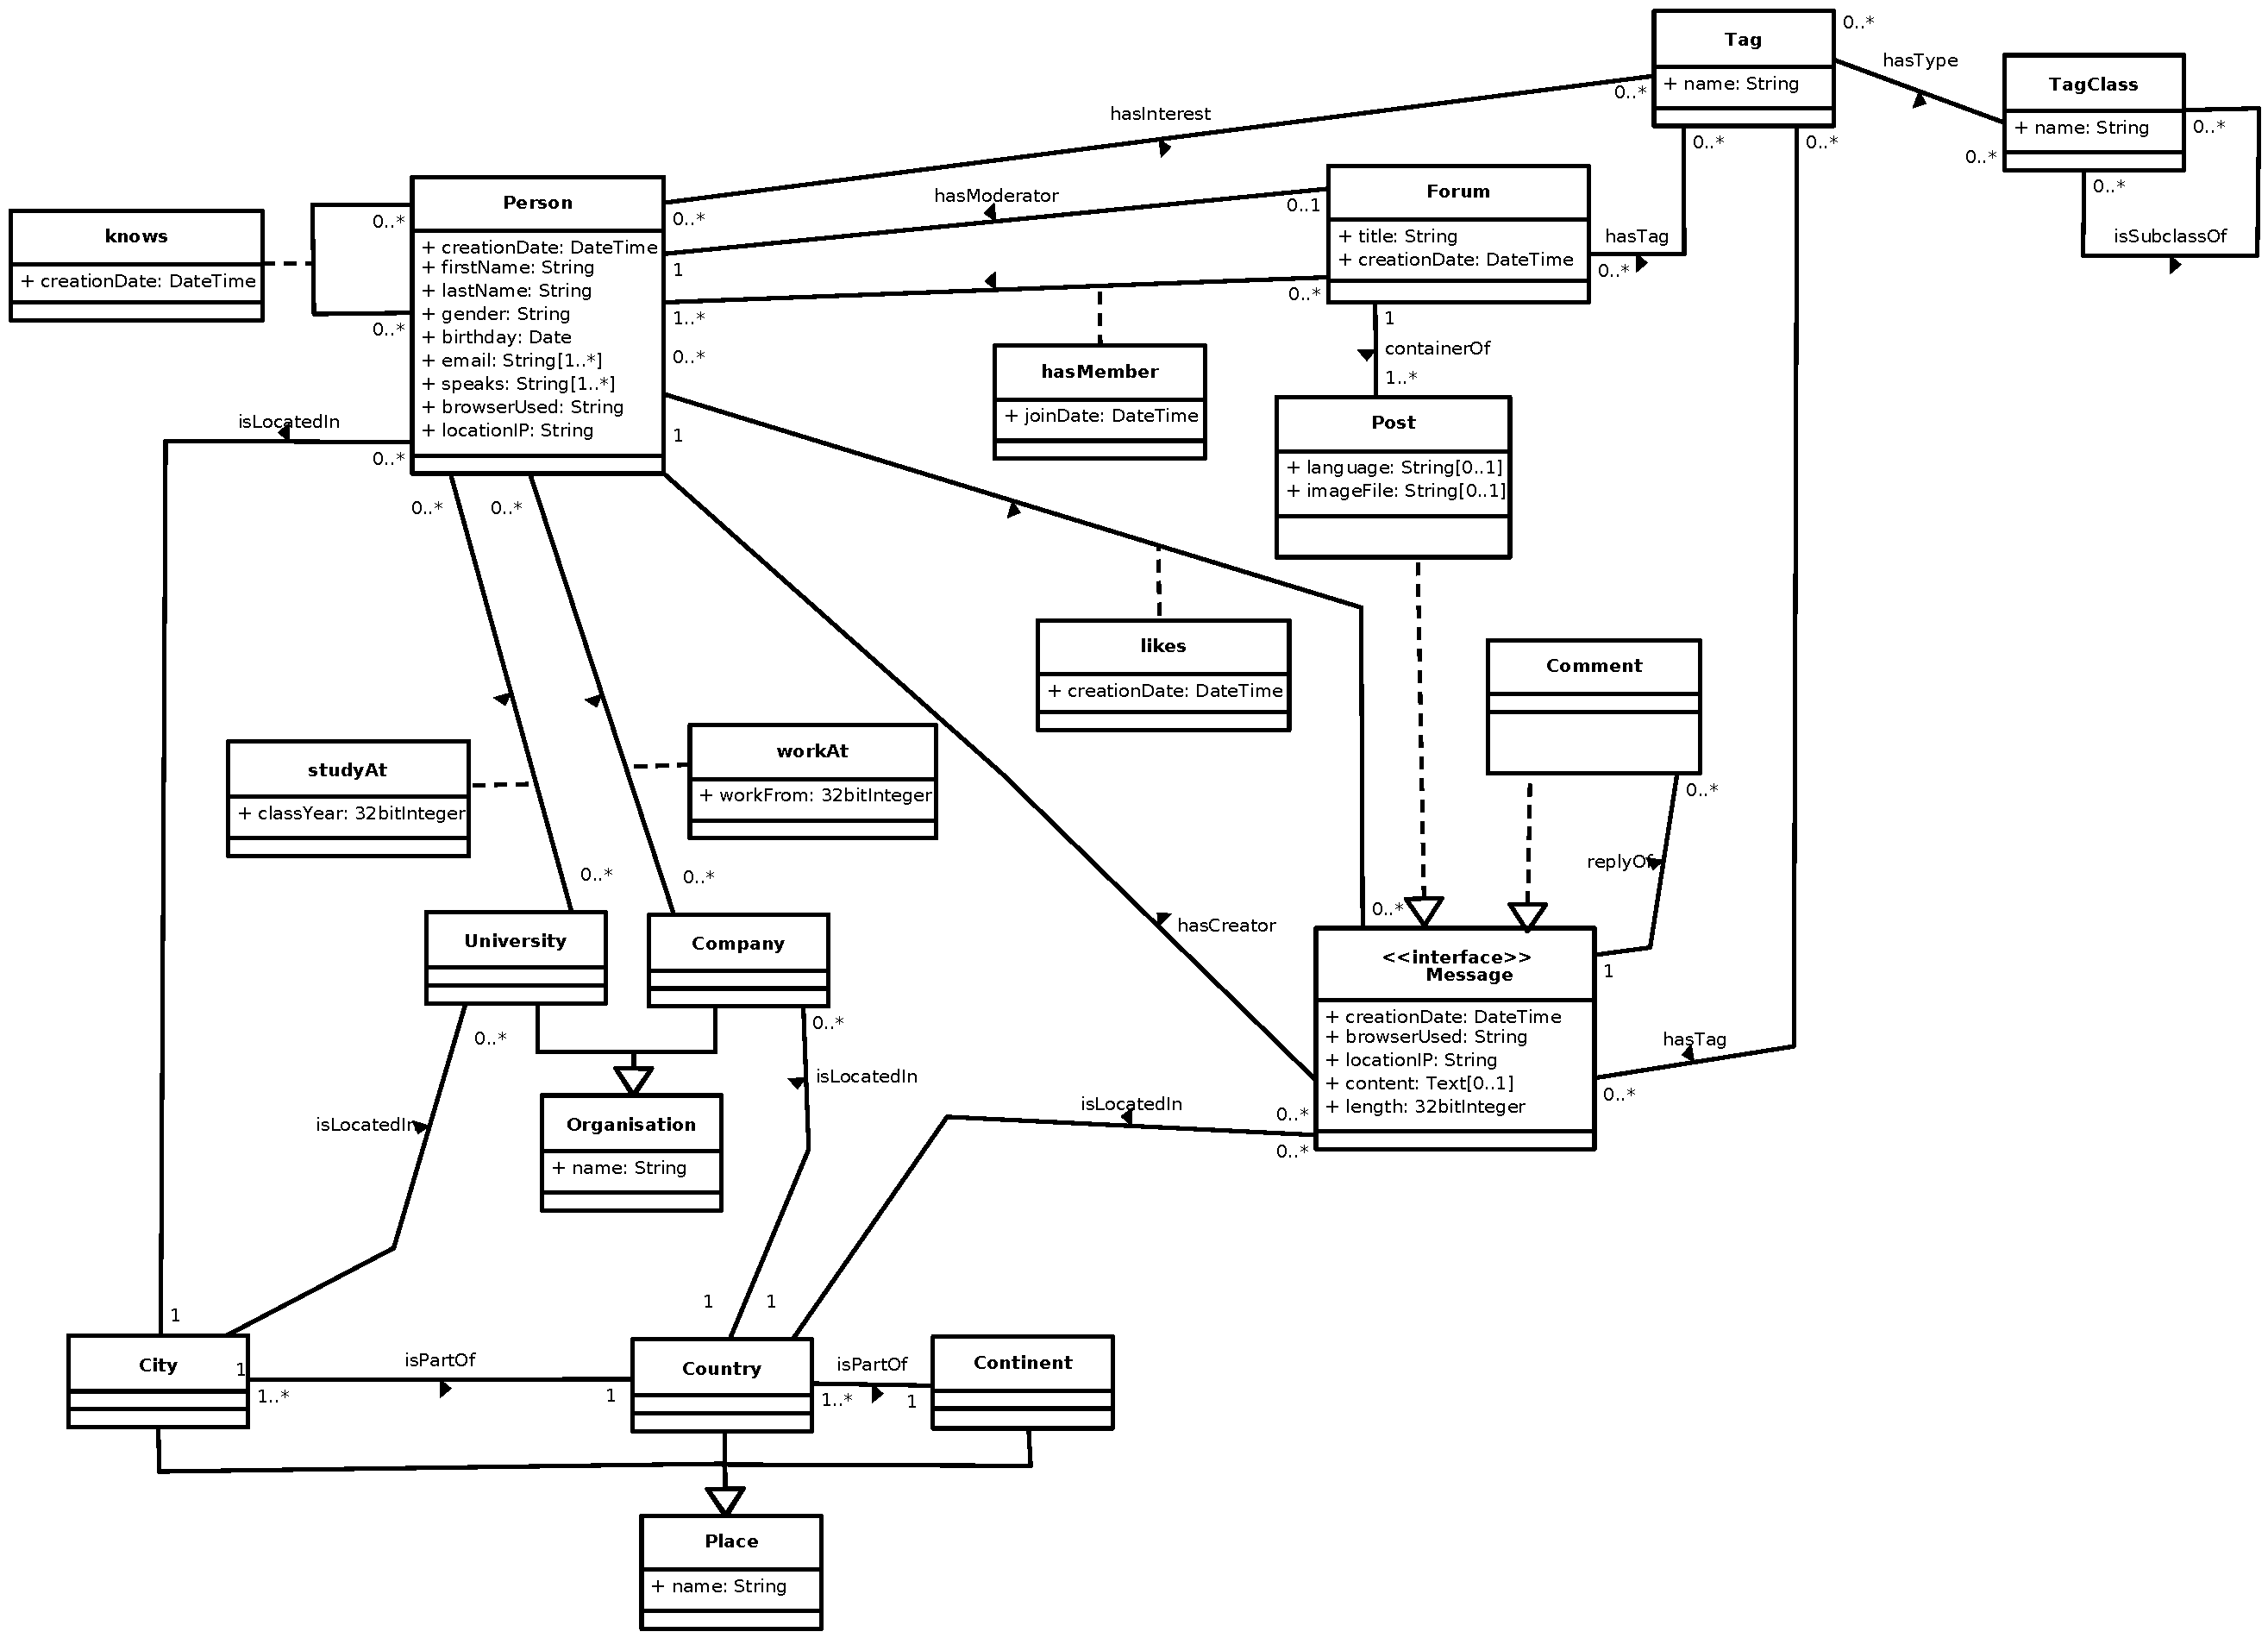
\includegraphics[width=0.9\linewidth]{figures/schema/schema.pdf}
%        \caption{The LDBC-SNB data schema}
%        \label{figure:schema}
%    \end{figure}
%\end{landscape}

\begin{figure}[p]
	\centering
	\rotatebox{90}{
		\begin{minipage}{\textheight}
			\centering
	        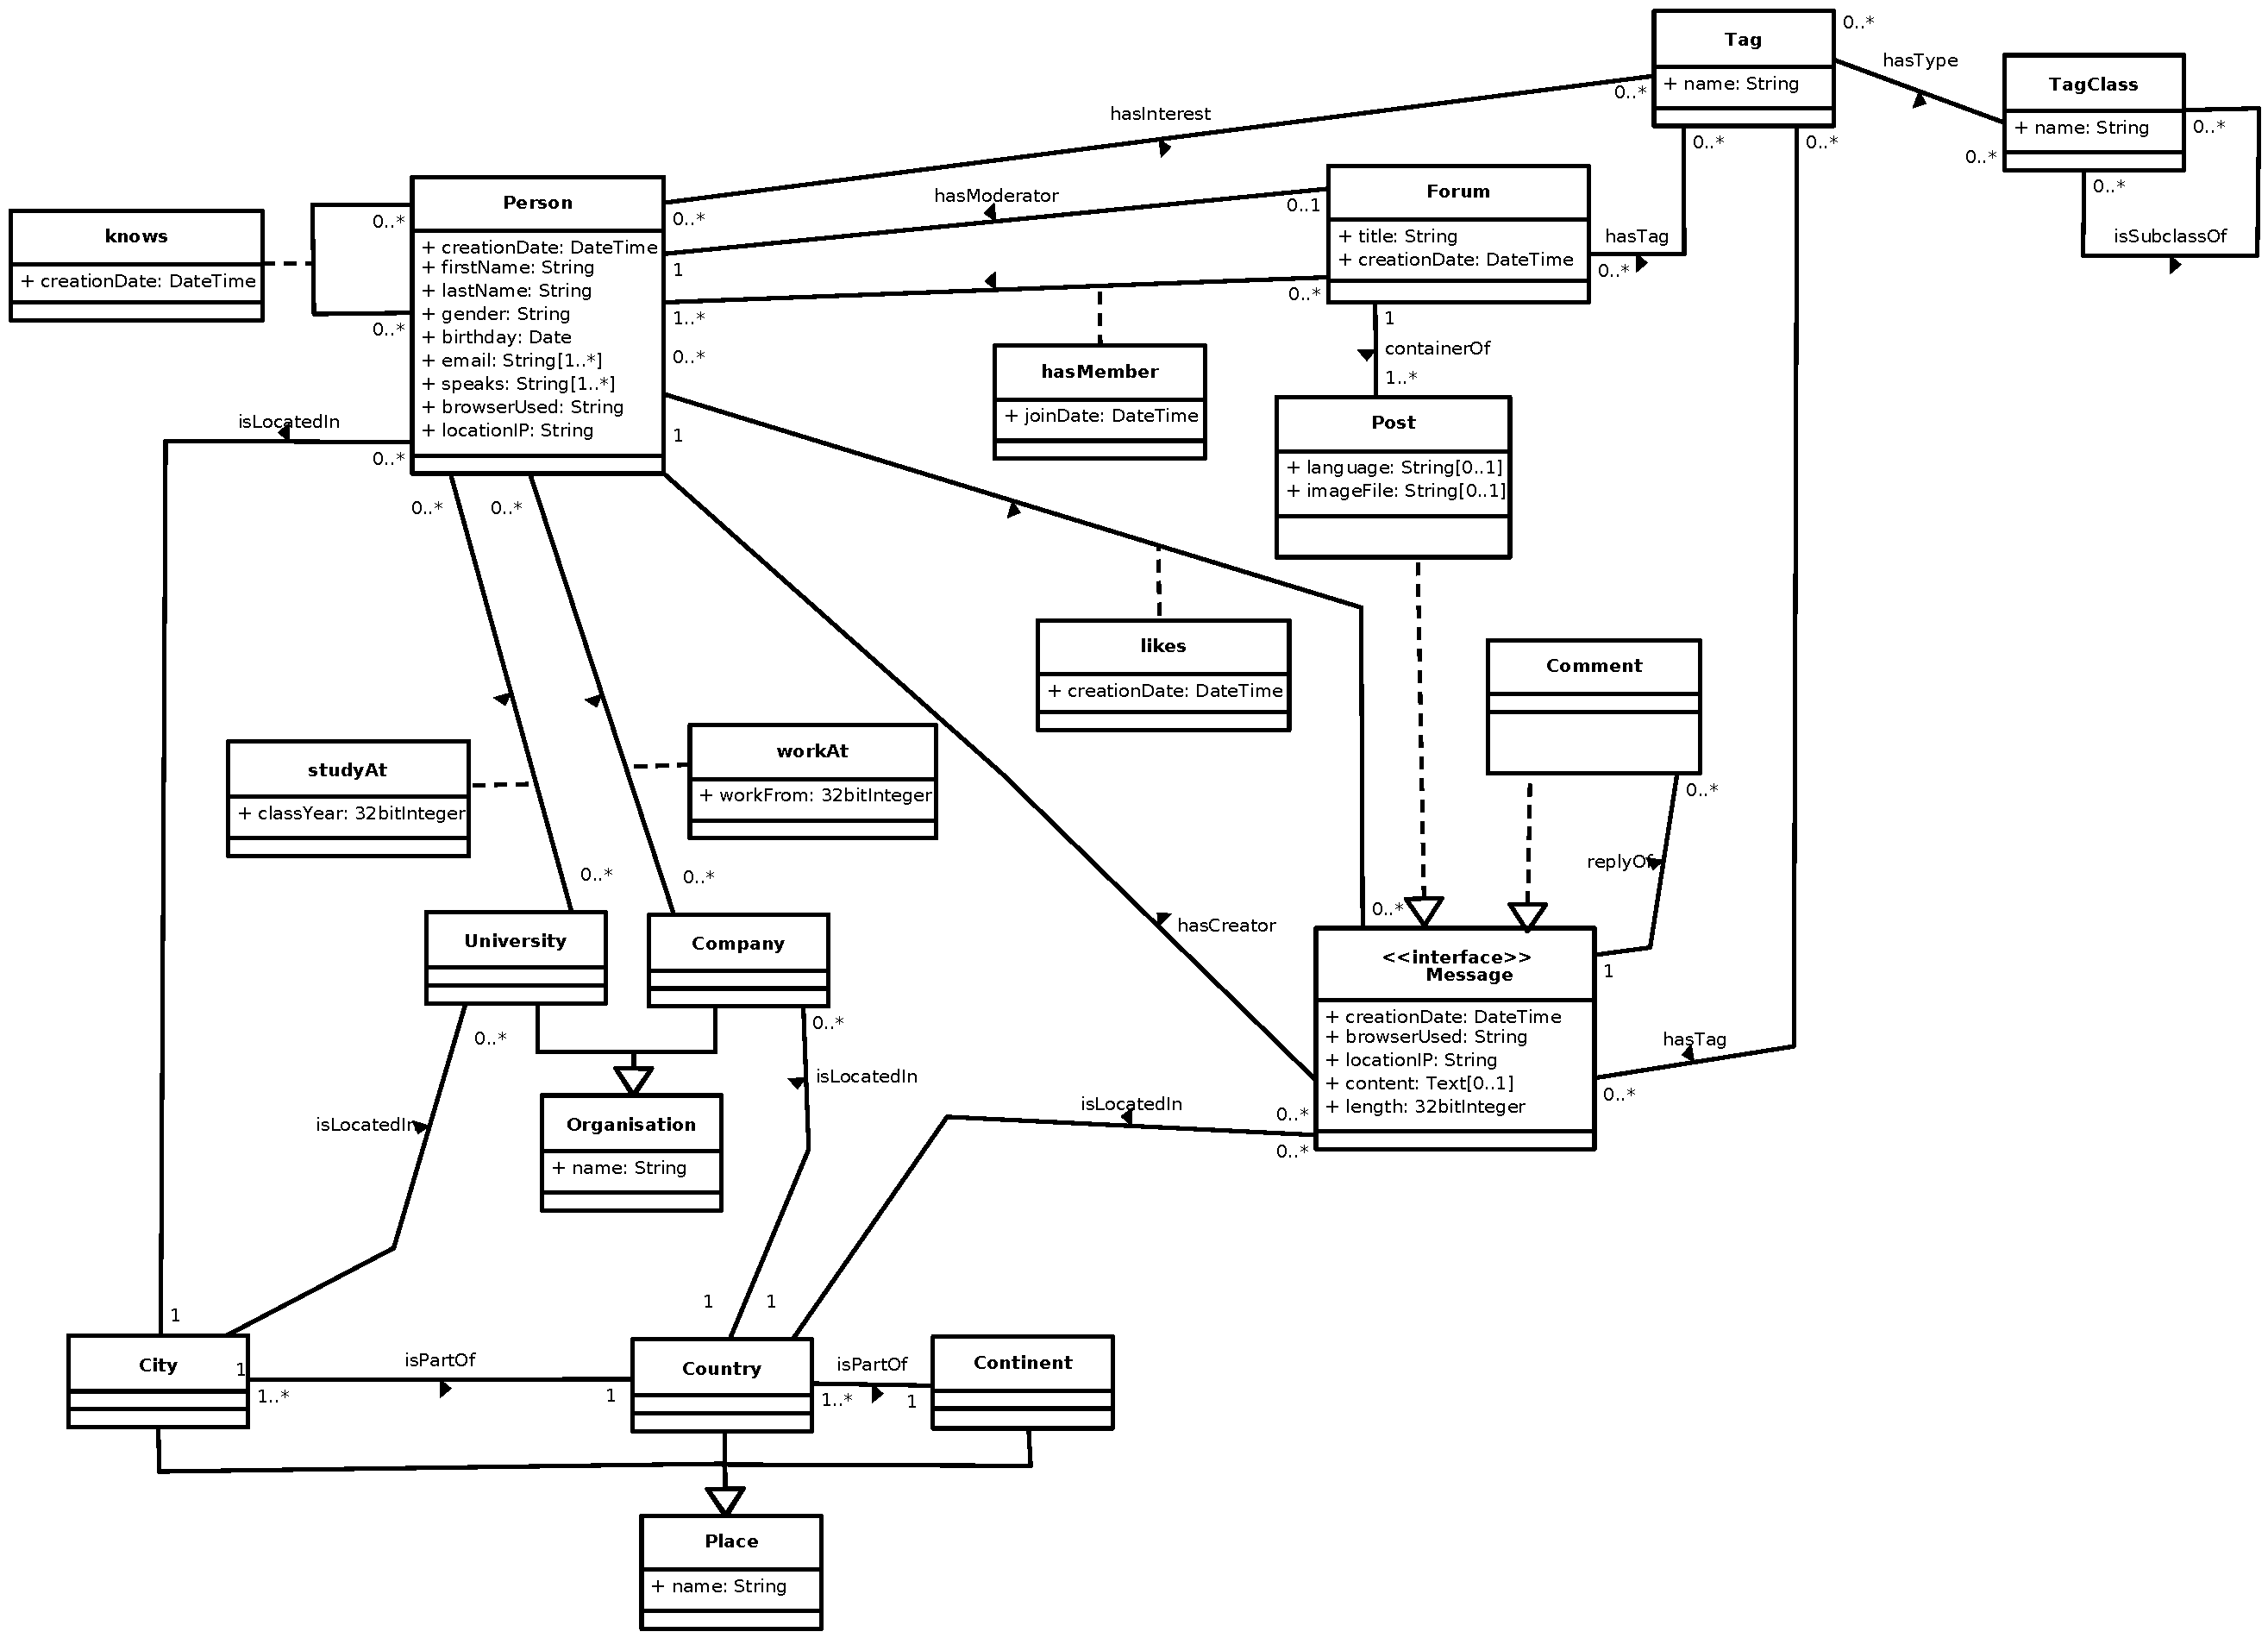
\includegraphics[width=0.9\linewidth]{figures/schema/schema.pdf}
    	    \caption{The LDBC-SNB data schema}
        	\label{figure:schema}
		\end{minipage}
	}
\end{figure}

The schema specifies different entities, their attributes and their relations.
All of them are described in the following sections.

\flushleft{\textbf{Textual Restrictions and Notes}}
\begin{itemize}
    \item Posts have content or imageFile. They have one of them but not both. The one they do not have is an empty string.
    \item Posts in a forum can be created by a non-member person if and only if that person is a modeartor.
\end{itemize}

\subsubsection{Entities}

{\flushleft \textbf{City:}} a sub-class of a Place, and represents a
city of the real world. City entities are used to specify where persons live,
as well as where universities operate.

{\flushleft \textbf{Comment:}} a sub-class of a Message, and represents a
comment made by a person to an existing message (either a Post or a Comment).

{\flushleft \textbf{Company:}} a sub-class of an Organization, and represents a company where persons work.


{\flushleft \textbf{Country:}} a sub-class of a Place, and represents a continent of the real world.


{\flushleft \textbf{Forum:}} a meeting point where people
post messages. Forums are characterized by the topics (represented as tags)
people in the forum are talking about. Although from the schema's perspective
it is not evident, there exist three different types of
forums: persons' personal walls, image albums, and groups. They are
distinguished by their titles. Table~\ref{table:forum} shows the attributes
of Forum entity.

\begin{table}[H]
    \begin{tabular}{|p{2.5cm}|p{2.5cm}|p{10.5cm}|}
        \hline
        \textbf{Attribute} & \textbf{Type} & \textbf{Description} \\
        \hline
        id & ID  & The identifier of the forum.\\
        \hline
        title & Long String  & The title of the forum.\\
        \hline
        creationDate & DateTime  & The date the forum was created\\
        \hline
    \end{tabular}
    \caption{Attributes of Forum entity.}
    \label{table:forum}
\end{table}

{\flushleft \textbf{Message:}} an abstract entity that represents a message
created by a person. Table~\ref{table:message} shows the attributes of Message
abstract entity.

\begin{table}[H]
    \begin{tabular}{|p{2.5cm}|p{2.5cm}|p{10.5cm}|}
        \hline
        \textbf{Attribute} & \textbf{Type} & \textbf{Description} \\
        \hline
        id & ID  & The identifier of the message.\\
        \hline
        browserUsed & String  & The browser used by the Person to create the message.\\
        \hline
        creationDate & DateTime  & The date the message was created.\\
        \hline
        locationIP & String  & The IP of the location from which the message was created.\\
        \hline
        content & Text[0..1]  & The content of the message.\\
        \hline
        length & 32-bit Integer  & The length of the content.\\
        \hline
    \end{tabular}
    \caption{Attributes of Message interface.}
    \label{table:message}
\end{table}

{\flushleft \textbf{Organization:}} an institution of the real
world. Table~\ref{table:organization} shows the attributes of Organization
entity.

\begin{table}[H]
    \begin{tabular}{|p{2.5cm}|p{2.5cm}|p{10.5cm}|}
        \hline
        \textbf{Attribute} & \textbf{Type} & \textbf{Description} \\
        \hline
        id & ID  & The identifier of the organization.\\
        \hline
        name & Long String  & The name of the organization.\\
        \hline
    \end{tabular}
    \caption{Attributes of Organization entity.}
    \label{table:organization}
\end{table}

{\flushleft \textbf{Person:}} the avatar a real world person creates
when he/she joins the network, and contains various information about the
person as well as network related information. Table~\ref{table:person} shows
the attributes of Person entity.

\begin{table}[H]
    \begin{tabular}{|p{2.5cm}|p{2.5cm}|p{10.5cm}|}
        \hline
        \textbf{Attribute} & \textbf{Type} & \textbf{Description} \\
        \hline
        id & ID  & The identifier of the person.\\
        \hline
        firstName & String  & The first name of the person.\\
        \hline
        lastName & String  & The last name of the person.\\
        \hline
        gender & String  & The gender of the person.\\
        \hline
        birthDay & Date  & The birthday of the person .\\
        \hline
        email & Long String[1..*]  & The set of emails the person has.\\
        \hline
        speaks & String[1..*]  & The set of languages the person speaks.\\
        \hline
        browserUser & String  & The browser used by the person when he/she registered to the social network.\\
        \hline
        locationIp & String  & The IP of the location from which the person was registered to the social network.\\
        \hline
        creationDate & DateTime  & The date the person joined the social network.\\
        \hline
    \end{tabular}
    \caption{Attributes of Person entity.}
    \label{table:person}
\end{table}


{\flushleft \textbf{Place:}} a place in the world.
Table~\ref{table:place} shows the attributes of Place entity.

\begin{table}[H]
    \begin{tabular}{|p{2.5cm}|p{2.5cm}|p{10.5cm}|}
        \hline
        \textbf{Attribute} & \textbf{Type} & \textbf{Description} \\
        \hline
        id & ID  & The identifier of the place.\\
        \hline
        name & Long String  & The name of the place.\\
        \hline
    \end{tabular}
    \caption{Attributes of Place entity.}
    \label{table:place}
\end{table}

{\flushleft \textbf{Post:}} a sub-class of Message, that is posted in a
forum. Posts are created by persons into the forums where they belong.
Posts contain either content or imageFile, always one of them but never both.
The one they do not have is an empty string.
Table~\ref{table:post} shows the attributes of Post entity.

\begin{table}[H]
    \begin{tabular}{|p{2.5cm}|p{2.5cm}|p{10.5cm}|}
        \hline
        \textbf{Attribute} & \textbf{Type} & \textbf{Description} \\
        \hline
        language & String[0..1]  & The language of the post.\\
        \hline
        imageFile & String[0..1]  & The image file of the post..\\
        \hline
    \end{tabular}
    \caption{Attributes of Post entity.}
    \label{table:post}
\end{table}

{\flushleft \textbf{Tag:}} a topic or a concept. Tags are used to
specify the topics of forums and posts, as well as the topics a person is
interested in. Table~\ref{table:tag} shows the attributes of Tag entity.

\begin{table}[H]
    \begin{tabular}{|p{2.5cm}|p{2.5cm}|p{10.5cm}|}
        \hline
        \textbf{Attribute} & \textbf{Type} & \textbf{Description} \\
        \hline
        id & ID  & The identifier of the tag.\\
        \hline
        name & Long String  &  The name of the tag.\\
        \hline
    \end{tabular}
    \caption{Attributes of Tag entity.}
    \label{table:tag}
\end{table}

{\flushleft \textbf{TagClass:}} a class or a category used to build
a hierarchy of tags. Table~\ref{table:tagclass} shows the attributes of TagClass
entity.

\begin{table}[H]
    \begin{tabular}{|p{2.5cm}|p{2.5cm}|p{10.5cm}|}
        \hline
        \textbf{Attribute} & \textbf{Type} & \textbf{Description} \\
        \hline
        id & ID  & The identifier of the tagclass.\\
        \hline
        name & Long String  &  The name of the tagclass.\\
        \hline
    \end{tabular}
    \caption{Attributes of TagClass entity.}
    \label{table:tagclass}
\end{table}

{\flushleft \textbf{University:}} a sub-class of Organization,
and represents an institution where persons study.

\subsubsection{Relations}

Relations connect entities of different types. Entities are defined by their ''id'' attribute.

\begin{longtable}{|p{2cm}|p{2.5cm}|p{2.5cm}|p{1cm}|p{7cm}|}
       \hline
        \textbf{Name} & \textbf{Tail} & \textbf{Head} & \textbf{Type} & \textbf{Description} \\
        \hline
        containerOf & Forum[1] & Post[1..*] & D & A Forum and a Post contained in it\\
        \hline
        hasCreator & Message[0..*] & Person[1] & D & A Message and its creator (Person)\\
        \hline
        hasInterest & Person[0..*] & Tag[0..*] & D & A Person and a Tag representing a topic the person is interested in\\
        \hline
        hasMember & Forum[0..*] &  Person[1..*] & D & A  Forum and a member (Person) of the forum
        \begin{itemize}
            \item \textbf{Attribute}: joinDate
            \item \textbf{Type:} DateTime
            \item \textbf{Description:} The Date the person joined the forum
        \end{itemize}
        \\
        \hline
        hasModerator & Forum[0..*] & Person[1] & D & A Forum and its moderator (Person) \\
        \hline
        hasTag & Message[0..*] & Tag[0..*] & D & A Message and a Tag representing the message's topic \\
        \hline
        hasTag & Forum[0..*] & Tag[0..*] & D & A Forum and a Tag representing the forum's topic \\
        \hline
        hasType & Tag[0..*] & TagClass[0..*] & D & A Tag and a TagClass the tag belongs to \\
        \hline
        isLocatedIn & Company[0..*] & Country[1] & D & A Company and its home Country \\
        \hline
        isLocatedIn & Message[0..*] & Country[1] & D & A Message and the Country from which it was issued \\
        \hline
        isLocatedIn & Person[0..*] & City[1] & D & A Person and their home City \\
        \hline
        isLocatedIn & University[0..*] & City[1] & D &  A University and the City where the university is \\
        \hline
        isPartOf & City[1..*] & Country[1] & D & A City and the Country it is part of \\
        \hline
        isPartOf & Country[1..*] & Continent[1] & D & A Country and the Continent it is part of \\
        \hline
        isSubclassOf & TagClass[0..*] & TagClass[0..*] & D & A TagClass its parent TagClass \\
        \hline
        knows & Person[0..*] & Person[0..*] & U & Two Persons that know each other
        \begin{itemize}
            \item \textbf{Attribute}: creationDate
            \item \textbf{Type:} DateTime
            \item \textbf{Description:}  The date the knows relation was established
        \end{itemize}
        \\
        \hline
        likes & Person[0..*] & Message[0..*] & D & A Person that likes a Message
        \begin{itemize}
            \item \textbf{Attribute}: creationDate
            \item \textbf{Type:} DateTime
            \item \textbf{Description:}  The date the like was issued
        \end{itemize}
        \\
        \hline
        replyOf & Comment[0..*] & Message[1] & D & A Comment and the Message it replies \\
        \hline
        studyAt & Person[0..*] & University[0..*] & D & A Person and a University it has studied
        \begin{itemize}
            \item \textbf{Attribute}: classYear
            \item \textbf{Type:} 32-bit Integer
            \item \textbf{Description:} The year the person graduated.
        \end{itemize}
        \\
        \hline
        workAt & Person[0..*] & Company[0..*] & D & A Person and a Company it works
        \begin{itemize}
            \item \textbf{Attribute:} workFrom
            \item \textbf{Type:} 32-bit Integer
            \item \textbf{Description:} The year the person started to work at that company
        \end{itemize}
        \\
        \hline
        \caption{Description of the data relations.}
        \label{table:relations}
\end{longtable}

%\subsection{Data Generation}\label{section:data_generation}
%
%LDBC-SNB provides DATAGEN (Data Base Generator), which produces synthetic
%datasets following the schema described above. Data
%produced mimics a social network's activity during a period of time. Three
%parameters determine the generated data: the number of persons, the number of
%years simulated, and the starting year of simulation. DATAGEN is defined by the
%following characteristics:
%
%\begin{itemize}
%    \item \textbf{Realism.} Data generated by DATAGEN mimics the
%        characteristics of those found in a real social network. In DATAGEN,
%        output attributes, cardinalities, correlations and distributions have
%        been finely tuned to reproduce a real social network in each of its
%        aspects On the one hand, it is aware of the  data and link distributions
%        found in a real social network such as Facebook. On the other hand, it
%        uses real data from DBPedia, such as property dictionaries, which are
%        used to ensure that attribute values are realistic and correlated.
%    \item \textbf{Scalability.} Since LDBC-SNB targets systems of different
%        scales and budgets, DATAGEN is capable of generating datasets of
%        different sizes, from a few Gigabytes to Terabytes. DATAGEN is
%        implemented following the MapReduce parallel paradigm, allowing the
%        generation of small datasets in single node machines, as well as large
%        datasets on commodity clusters.
%    \item \textbf{Determinism.} DATAGEN is deterministic regardless of the number
%        of cores/machines used to produce the data. This important feature
%        guarantees that all Test Sponsors will face the same dataset,
%        thus, making the comparisons between different systems fair and the
%        benchmarks' results reproducible.
%    \item \textbf{Usability.} LDBC-SNB is designed to have an affordable entry
%        point. As such, DATAGEN's design is  severely influenced by this
%        philosophy, and therefore it is designed to be as easy to use as
%        possible.
%\end{itemize}
%
%
%\subsubsection{Resource Files}
%
%DATAGEN uses a set of resource files with data
%extracted from DBpedia. Conceptually, DATAGEN generates attribute's
%values following a property dictionary model that is defined by
%
%\begin{itemize}
%    \item a dictionary $D$
%    \item a ranking function $R$
%    \item a probability function $F$
%\end{itemize}
%
%Dictionary D is a fixed set of values. The ranking function R is a bijection
%that assigns to each value in a dictionary a unique rank between 1 and |$D$|.
%The probability density function $F$ specifies how the data generator chooses
%values from dictionary $D$ using the rank for each term in the dictionary. The
%idea to have a separate ranking and probability function is motivated by the
%need of generating correlated values: in particular, the ranking function is
%typically parameterized by some parameters: different parameter values result
%in different rankings. For example, in the case of a dictionary of property
%firstName, the popularity of first names, might depend on the gender, country
%and birthDate properties. Thus, the fact that the popularity of first names in
%different countries and times is different, is reflected by the different ranks
%produced by function $R$ over the full dictionary of names.  DATAGEN uses a
%dictionary for each literal property, as well as ranking functions for all
%literal properties. These are materialized in a set of resource files, which
%are described in Table~\ref{table:property_dictionaries}.
%
%\begin{table}[H]
%\begin{tabular}{|p{4cm}|p{12cm}|}
%    \hline
%    \textbf{Resource Name} & \textbf{Description} \\
%    \hline
%    Browsers & Contains a list of web browsers and their probability to be used. It is used to set the browsers used by the users.\\
%    \hline
%    Cities by Country & Contains a list of cites and the country they belong. It is used to assign cities to users and universities.\\
%    \hline
%    Companies by Country & Contains the set of companies per country. It is used to set the countries where companies operate.\\
%    \hline
%    Countries & Contains a list of countries and their populations. It is used to obtain the amount of people generated for each country.\\
%    \hline
%    Emails & Contains the set of email providers. It is used to generate the email accounts of persons.\\
%    \hline
%    IP Zones & Contains the set of IP ranges assigned to each country. It is used to assign the IP addresses to users.\\
%    \hline
%    Languages by Country & Contains the set of languages spoken in each country. It is used to set the languages spoken by each user.\\
%    \hline
%    Name by Country & Contains the set of names and the probability to appear in each country. It is used to assign names to persons, correlated with their countries.\\
%    \hline
%    Popular places by Country & Contains the set of popular places per country. These are used to set where images attached to posts are taken from.\\
%    \hline
%    Surnames' by Country & Contains the set of surnames and the probability to appear in each country. It is used to assign surnames to persons, correlated with their countries.\\
%    \hline
%    Tags by Country & Contains a set of tags and their probability to appear in each country. It is used to assign the interests to persons and forums.\\
%    \hline
%    Tag Classes & Contains, for each tag, the classes it belongs to.\\
%    \hline
%    Tag Hierarchies & Contains, for each tagClass, their parent tagClass.\\
%    \hline
%    Tag Matrix & Contains, for each tag, the correlation probability with the other tags. It is used enrich the tags associated to messages.\\
%    \hline
%    Tag Text & Contains, for each tag, a text. This is used to generate the text for messages.\\
%    \hline
%    Universities by City & Contains the set of universities per city. It is used to set the cities where universities operate.\\
%    \hline
%\end{tabular}
%    \caption{Resource files}
%    \label{table:property_dictionaries}
%\end{table}
%
%\subsubsection{Graph Generation}
%
%Figure~\ref{figure:generation_process} conceptually depicts the full data
%generation process. The first step loads all the dictionaries and resource
%files, and initializes the DATAGEN parameters.  Second, it generates all the
%Persons in the graph, and the minimum necessary information to operate. Part of
%these information are the interests of the persons, and the number of knows
%relationships of every person, which is guided by a degree distribution
%function similar to that found in Facebook~\cite{facebook_anatomy}.
%
%The next three steps are devoted to the creation of knows relationships.  An
%important aspect of real social networks, is the fact that similar persons
%(with similar interests and behaviors) tend to be connected. This is known as
%the Homophily principle~\cite{mcpherson2001birds}, and implies the presence of
%a larger amount of triangles than that expected in a random network. In order
%to reproduce this characteristic, DATAGEN generates the edges by means of
%correlation dimensions.  Given a person, the probability to be connected to
%another person is typically skewed with respect to some similarity between the
%persons. That is, for a person $n$ and for a small set of persons that are
%somehow similar to it, there is a high connectivity probability, whereas for
%most other persons, this probability is quite low. This knowledge is
%exploited by DATAGEN to reproduce correlations.
%
%\begin{figure}[H]
%    \centering
%    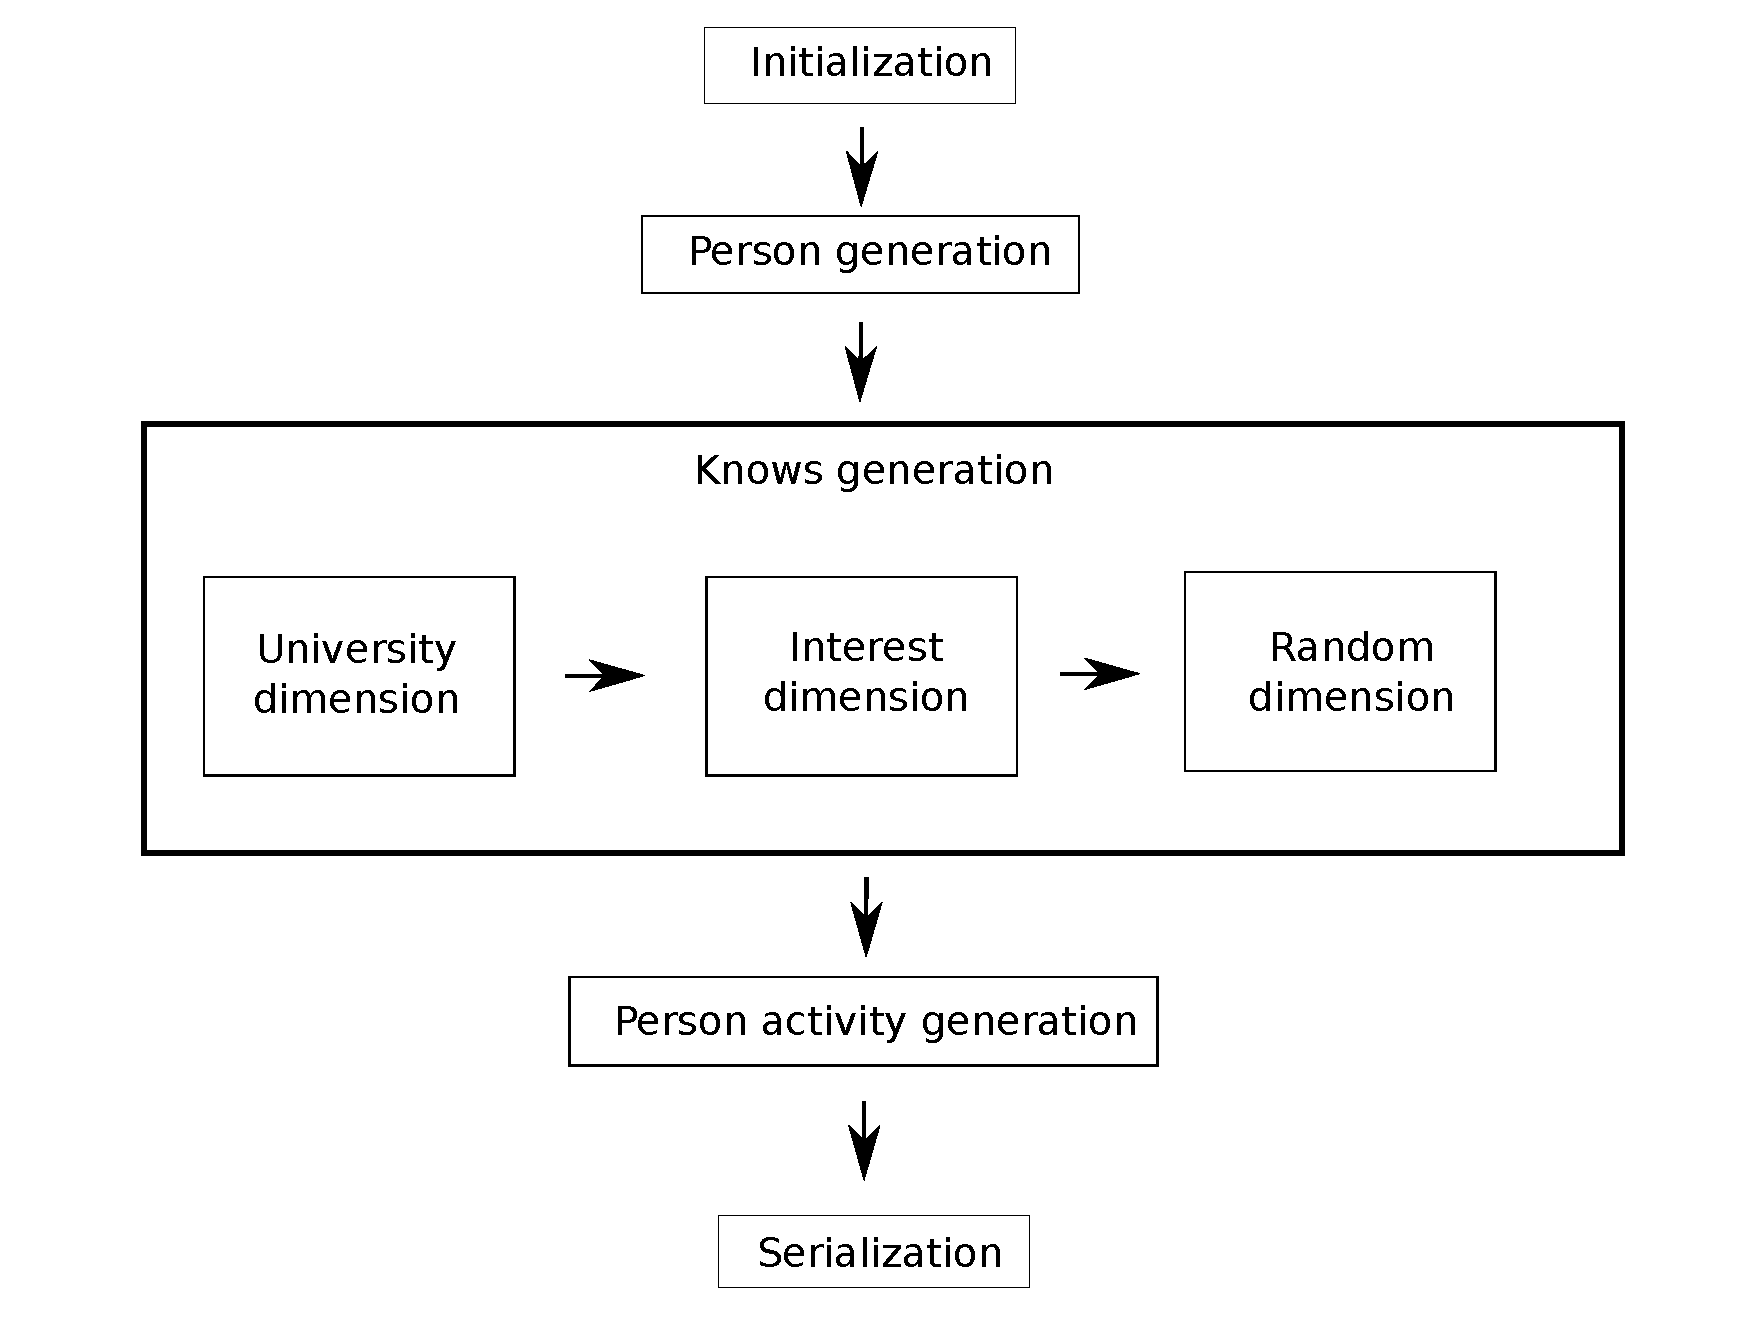
\includegraphics[width=1\linewidth]{figures/sndg/execution.pdf}
%    \caption{The DATAGEN generation process.}
%    \label{figure:generation_process}
%\end{figure}
%
%Given a similarity function $M(x) : n → [0, \infty]$ that gives a score to a person,
%with the characteristic that two similar persons will have similar scores, we
%can sort all the persons by function $M$ and compare a person n against only the
%W neighboring persons in the sorted array. The consequence of this approach is
%that similar persons are grouped together, and the larger the
%distance between two persons indicates a monotonic increase in their similarity
%difference. In order to choose the persons to connect, DATAGEN uses a geometric
%probability distribution that provides a probability for picking persons to
%connect, that are between 1 and $W$ positions apart in the similarity
%ranking.
%
%Similarity functions and probability distribution functions over ranked
%distance drive what kind of persons will be connected with an edge, not how
%many. As stated above, the number of friends of a person is determined by a
%Facebook-like distribution. The edges that will be connected to a person $n$,
%are selected by randomly picking the required number of edges according to the
%correlated probability distributions as discussed before. In the case that
%multiple correlations exist, another probability function is used to divide the
%intended number of edges between the various correlation dimensions. In DATAGEN,
%three correlated dimensions are chosen: the first one depends on where the
%person studied and when, and the second correlation dimension depends on the
%interests of the person, and the third one is random (to reproduce the random
%noise present in real data). Thus, DATAGEN has a Facebook-like distributed node
%degree, and a predictable (but not fixed) average split between the reasons for
%creating edges.
%
%In the next step, person's activity, in the form of forums, posts and comments
%is created. DATAGEN reproduces the fact that people with a larger number of
%friends have a higher activity, and hence post more photos and comments to a
%larger number of posts. Another important characteristic of real users'
%activity in social network, are time correlations.  Usually, users' posts
%creation in a social network is driven by real world events.  For
%instance, one may think about an important event such as the elections in a
%country, or a natural disaster. Around the time these events occur, network
%activity about these events' topics sees an increase in volume. DATAGEN
%reproduces these characteristics with the simulation of what we name as
%flashmob events.  Several events are generated randomly at the beginning of the
%generation process, which are assigned a random tag, and are given a time and
%an intensity which represents the repercussion of the event in the real world.
%When persons' posts are created, some of them are classified as flashmob posts,
%and their topics and dates are assigned based on the generated flashmob events.
%The volume of activity around this events is modeled following a model similar
%to that described in~\cite{flashmobs}. Furthermore, in order to reproduce the
%more uniform every day's user activity, DATAGEN also generates post uniformly
%distributed along all the simulated time.
%
%Finally, in the last step the data is serialized into the output files.
%
%\subsubsection{Implementation Details}
%
%DATAGEN is implemented using the MapReduce parallel paradigm. In MapReduce, a
%Map function runs on different parts of the input data, in parallel and on many
%node clusters. This function processes the input data and produces for each
%result a key. Reduce functions then obtain this data and Reducers run in
%parallel on many cluster nodes. The produced key simply determines the Reducer
%to which the results are sent. The use of the MapReduce paradigm allows the
%generator to scale considerably, allowing the generation of huge datasets by
%using clusters of machines.
%
%In the case of DATAGEN, the overall process is divided into three MapReduce jobs.
%In the first job, each mapper generates a subset of the persons of the graph. A
%key is assigned to each person using one of the similarity functions described
%above. Then, reducers receive the the key-value pairs sorted by the key,
%generate the knows relations following the described windowing process, and
%assign to each person a new key based on another similarity function, for the
%next MapReduce pass.  This process can be successively repeated for additional
%correlation dimension.  Finally, the last reducer generates the remaining
%information such as forums, posts and comments.
%

\subsection{Output Data}

DATAGEN produces outputs three different items:
\begin{itemize}
  \item \textbf{Dataset}: The dataset to be bulk loaded by the SUT. It
    corresponds to roughly the 90\% of the total generated network.
  \item \textbf{Update Streams}: A set of update streams containing update
    queries, which are used by the driver to generate the update queries of the
    workloads. This update
    streams correspond to the remaining 10\% of the generated dataset.
  \item \textbf{Substitution Parameters}: A set of files containing the
    different parameter bindings that will be used by the driver to generate the
    read queries of the workloads.
\end{itemize}

The SUT have to take care only of the generated Dataset to be bulk loaded.
Three different formats are supported by DATAGEN:

\begin{itemize}
  \item \textbf{CSV:} Data output in CSV format, one file per different entity and on file
    per different relation. Also, there is a file por those attributes whose
    cardinality is larger than one (\ie Person.email, Person.speaks, \etc).
  \item \textbf{CSVMergeForeign:} Similar to CSV format, but in this case, those
    relations of the form 1 to 1 and 1 to N, are stored in the tail entity file as
    a foreign keys.
  \item \textbf{Turtle:} Dataset in turtle format for RDF systems.
\end{itemize}



\subsubsection{CSV}

This is a comma separated format. Each entity, relation and properties with a
cardinality larger than one, are output in a separate file. Generated files are
summarized at Table~\ref{table:csv}.  Depending on the number of threads used
for generating the dataset, the number of files varies, since there is a file
generated per thread. The * in the file names indicates a number between 0 and
$\mathit{NumberOfThreads}-1$.

\begin{table}[htbp]
	\centering
	\rotatebox{90}{
	\begin{minipage}[c]{\textheight}
        \footnotesize
        \centering
        \begin{tabular}{|p{5cm}|p{19cm}|}
            \hline
            \textbf{File} & \textbf{Content} \\
            \hline
            comment\_*.csv & id | creationDate | locationIP | browserUsed | content | length |\\
            \hline
            comment\_hasCreator\_person\_*.csv & Comment.id | Person.id |\\
            \hline
            comment\_isLocatedIn\_place\_*.csv & Comment.id | Place.id |\\
            \hline
            comment\_replyOf\_comment\_*.csv & Comment.id | Comment.id |\\
            \hline
            comment\_replyOf\_post\_*.csv &  Comment.id | Post.id |\\
            \hline
            forum\_*.csv & id | title | creationDate |\\
            \hline
            forum\_containerOf\_post\_*.csv & Forum.id | Post.id |\\
            \hline
            forum\_hasMember\_person\_*.csv & Forum.id | Person.id | joinDate |\\
            \hline
            forum\_hasModerator\_person\_*.csv & Forum.id | Person.id |\\
            \hline
            forum\_hasTag\_tag\_*.csv & Forum.id | Tag.id |\\
            \hline
            organization\_*.csv & id | type({"university", "company"}) | name | url |\\
            \hline
            organisation\_isLocatedIn\_place\_*.csv & Organisation.id | Place.id |\\
            \hline
            person\_*.csv & id | firstName | lastName | gender | birthday | creationDate | locationIP | browserUsed |\\
            \hline
            person\_email\_emailaddress\_*.csv & Person.id | email |\\
            \hline
            person\_hasInterest\_tag\_*.csv &  Person.id | Tag.id |\\
            \hline
            person\_isLocatedIn\_place\_*.csv & Person.id | Place.id |\\
            \hline
            person\_knows\_person\_*.csv & Person.id | Person.id | creationDate |\\
            \hline
            person\_likes\_comment\_*.csv & Person.id | Post.id | creationDate |\\
            \hline
            person\_likes\_post\_*.csv & Person.id | Post.id | creationDate |\\
            \hline
            person\_speaks\_language\_*.csv & Person.id | language |\\
            \hline
            person\_studyAt\_organisation\_*.csv & Person.id | Organisation.id | classYear |\\
            \hline
            person\_workAt\_organisation\_*.csv &  Person.id | Organisation.id | workFrom |\\
            \hline
            place\_*.csv & id | name | url | type({"city", "country", "continent"}) |\\
            \hline
            place\_isPartOf\_place\_*.csv & Place.id | Place.id |\\
            \hline
            post\_*.csv & id | imageFile | creationDate | locationIP | browserUsed | language | content | length |\\
            \hline
            post\_hasCreator\_person\_*.csv & Post.id | Person.id |\\
            \hline
            post\_hasTag\_tag\_*.csv & Post.id | Tag.id |\\
            \hline
            post\_isLocatedIn\_place.csv & Post.id | Place.id |\\
            \hline
            tag\_*.csv & id | name | url | \\
            \hline
            tag\_hasType\_tagclass\_*.csv & Tag.id | TagClass.id |\\
            \hline
            tagclass\_*.csv & id | name | url | \\
            \hline
            tagclass\_isSubclassOf\_tagclass\_*.csv & TagClass.id | TagClass.id |\\
            \hline
        \end{tabular}
        \caption{Files output by CSV serializer}
        \label{table:csv}
	\end{minipage}
	}
\end{table}




\subsubsection{CSV\_MERGE\_FOREIGN}

This is a comma separated format. It is similar to CSV, but those relations
connecting two entities A and B, where an entity A has a cardinality of one, A
is output as a column of entity B. Generated files are summarized at
Table~\ref{table:csv_merge_foreign}. Depending on the number of threads used for generating
the dataset, the number of files varies, since there is a file generated per
thread. The * in the file names indicates a number between 0 and $\mathit{NumberOfThreads}-1$.

\begin{table}[htbp]
	\centering
	\rotatebox{90}{
		\begin{minipage}[c]{\textheight}
        \footnotesize
        \centering
        \begin{tabular}{|p{5cm}|p{19cm}|}
            \hline
            \textbf{File} & \textbf{Content} \\
            \hline
            comment\_*.csv & id | creationDate | locationIP | browserUsed | content | length | creator | place | replyOfPost | replyOfComment |\\
            \hline
            forum\_*.csv & id | title | creationDate | moderator |\\
            \hline
            forum\_hasMember\_person\_*.csv & Forum.id | Person.id | joinDate |\\
            \hline
            forum\_hasTag\_tag\_*.csv & Forum.id | Tag.id |\\
            \hline
            organization\_*.csv & id | type({"university", "company"}) | name | url |\\
            \hline
            organisation\_isLocatedIn\_place\_*.csv & Organisation.id | Place.id |\\
            \hline
            person\_*.csv & id | firstName | lastName | gender | birthday | creationDate | locationIP | browserUsed | place |\\
            \hline
            person\_email\_emailaddress\_*.csv & Person.id | email |\\
            \hline
            person\_hasInterest\_tag\_*.csv &  Person.id(Long) | Tag.id |\\
            \hline
            person\_knows\_person\_*.csv & Person.id | Person.id  | creationDate |\\
            \hline
            person\_likes\_comment\_*.csv & Person.id | Post.id | creationDate |\\
            \hline
            person\_likes\_post\_*.csv & Person.id | Post.id | creationDate |\\
            \hline
            person\_speaks\_language\_*.csv & Person.id | language |\\
            \hline
            person\_studyAt\_organisation\_*.csv & Person.id | Organisation.id | classYear |\\
            \hline
            person\_workAt\_organisation\_*.csv &  Person.id | Organisation.id | workFrom |\\
            \hline
            place\_*.csv & id | name | url | type({"city", "country", "continent"}) |\\
            \hline
            place\_isPartOf\_place\_*.csv & Place.id | Place.id |\\
            \hline
            post\_*.csv & id | imageFile | creationDate | locationIP | browserUsed | language | content | length | creator | Forum.id | place |\\
            \hline
            post\_hasTag\_tag\_*.csv & Post.id | Tag.id |\\
            \hline
            tag\_*.csv & id | name | url | \\
            \hline
            tag\_hasType\_tagclass\_*.csv & Tag.id | TagClass.id |\\
            \hline
            tagclass\_*.csv & id | name | url | \\
            \hline
            tagclass\_isSubclassOf\_tagclass\_*.csv & TagClass.id | TagClass.id |\\
            \hline
        \end{tabular}
        \caption{Files output by CSV\_MERGE\_FOREIGN serializer}
        \label{table:csv_merge_foreign}
	\end{minipage}
}
\end{table}


\subsubsection{Turtle}

This is the standard Turtle\footnote{Description of
the Turtle RDF format http://www.w3.org/TR/turtle/} format. DATAGEN outputs
two files: \texttt{0\_ldbc\_socialnet\_static\_dbp.ttl} and \texttt{0\_ldbc\_socialnet.ttl}.

\subsection{Scale Factors}

LDBC-SNB defines a set of scale factors (SFs), targeting systems of different
sizes and budgets.  SFs are computed based on the ASCII size in Gigabytes of
the generated output files using the CSV serializer. For example, SF 1 weights roughly 1~GB in CSV
format, SF 3 weights roughly 3~GB and so on and so forth.  The proposed SFs are
the following: 1, 3, 10, 30, 100, 300, 1000. The Test Sponsor may select the SF
that better fits their needs, by properly configuring the DATAGEN.
% , as described in Section~\ref{section:data_generation}.

The size of the resulting dataset, is mainly affected by the following
configuration parameters: the number of persons and the number of years
simulated. Different SFs are computed by scaling the number of Persons in
the network, while fixing the number of years simulated.
Table~\ref{tab:snsize} shows the parameters used in each of the SFs.

\begin{table}[H]
\centering
\begin{tabular}{|c||r|r|r|r|r|r|r|}
\hline  Scale Factor  & 1 &  3 & 10 & 30 & 100 & 300 & 1000 \\
\hline  \# of Persons  & 11K &  27K & 73K & 182K & 499K & 1.25M & 3.6M \\
\hline  \# of Years  & 3 &  3 & 3 & 3 & 3 & 3 & 3 \\
\hline  Start Year & 2010 &  2010 & 2010 & 2010 & 2010 & 2010 & 2010 \\
\hline
\end{tabular}
\centering
\caption{Parameters of each scale factor.}
\label{tab:snsize}
\end{table}

For example, SF 30 consists of the activity of a social network of 182K users
during a period of three years, starting from 2010.

%In
%Appendix~\ref{appendix:scale_factors}, we show the statistics of each of the
%proposed SFs in detail, including distributions for some of the relations.

%%%%%%%%%%%%%%%%%%%%%%%%%%%%%%%%%%%%%%%%%%%%%%%%%%%%%%%%%%%%%%%%%%%%%%%%%%%%%%
%%%%%%%%%%%%%%%%%%%%%%%%%%%%%%%%%%%%%%%%%%%%%%%%%%%%%%%%%%%%%%%%%%%%%%%%%%%%%%
%%%%%%%%%%%%%%%%%%%%%%%%%%%%%%%%%%%%%%%%%%%%%%%%%%%%%%%%%%%%%%%%%%%%%%%%%%%%%%

\chapter{Workloads}
\label{section:workloads}

%%%%%%%%%%%%%%%%%%%%%%%%%%%%%%%%%%%%%%%%%%%%%%%%%%%%%%%%%%%%%%%%%%%%%%%%%%%%%%
%%%%%%%%%%%%%%%%%%%%%%%%%%%%%%%%%%%%%%%%%%%%%%%%%%%%%%%%%%%%%%%%%%%%%%%%%%%%%%
%%%%%%%%%%%%%%%%%%%%%%%%%%%%%%%%%%%%%%%%%%%%%%%%%%%%%%%%%%%%%%%%%%%%%%%%%%%%%%

\section{Query Description Format}
\label{sub:queries_structure}
Queries are described in natural language using a well-defined structure that consists of three sections:
\textit{description}, a concise textual description of the query;
\textit{parameters}, a list of input parameters and their types;
and \textit{results}, a list of expected results and their types.
The syntax used in \textit{parameters} and \textit{results} sections is as follows:

\begin{itemize}
    \item \textbf{Entity}: entity type in the dataset.\\
        One word, possibly constructed by appending multiple words together, starting with uppercase character and following the camel case notation,
        \eg \texttt{TagClass} represents an entity of type ``TagClass''.
    \item \textbf{Relationship}: relationship type in the dataset.\\
        One word, possibly constructed by appending multiple words together, starting with lowercase character and following the camel case notation,
        and surrounded by arrow to communicate direction,
        \eg \mbox{\texttt{-worksAt->}} represents a directed relationship of type ``worksAt''.
    \item \textbf{Attribute}: attribute of an entity or relationship in the dataset.\\
        One word, possibly constructed by appending multiple words together, starting with lowercase character and following the camel case notation,
        and prefixed by a ``.'' to dereference the entity/relationship,
        \eg \texttt{Person.firstName} refers to ``firstName'' attribute on the ``Person'' entity,
        and \mbox{\texttt{-studyAt->.classYear}} refers to ``classYear'' attribute on the ``studyAt'' relationship.
    \item \textbf{Unordered Set}: an unordered collection of distinct elements.\\
        Surrounded by \{ and \} braces, with the element type between them,
        \eg \texttt{\{String\}} refers to a set of strings.
    \item \textbf{Ordered List}: an ordered collection where duplicate elements are allowed.\\
        Surrounded by [ and ] braces, with the element type between them,
        \eg \texttt{[String]} refers to a list of strings.
    \item \textbf{Ordered Tuple}: a fixed length, fixed order list of elements, where elements at each position of the tuple have predefined, possibly different, types. \\
        Surrounded by < and > braces, with the element types between them in a specific order
        \eg \texttt{<String, Boolean>} refers to a 2-tuple containing a string value in the first element and a boolean value in the second,
        and \texttt{[<String, Boolean>]} is an ordered list of those 2-tuples.
\end{itemize}

\paragraph{Categorization of results.} Results are categorized according to their source of origin:

\begin{itemize}
	\item \textbf{Raw} (\texttt{R}), if the result is returned with an unmodified value and type.
	\item \textbf{Calculated} (\texttt{C}), if the result is calculated from other values and conditions.
	\item \textbf{Aggregated} (\texttt{A}), if the result is an aggregated value, \eg a count or a sum of another value. If a result is both calculated and aggregated (\eg $\mathsf{count(x) + count(y)}$ or $\mathsf{avg(x + y)}$), it is considered an aggregated result.
	\item \textbf{Meta} (\texttt{M}), if the result is based on type information, \eg the type of the node.
\end{itemize}


%%%%%%%%%%%%%%%%%%%%%%%%%%%%%%%%%%%%%%%%%%%%%%%%%%%%%%%%%%%%%%%%%%%%%%%%%%%%%%
%%%%%%%%%%%%%%%%%%%%%%%%%%%%%%%%%%%%%%%%%%%%%%%%%%%%%%%%%%%%%%%%%%%%%%%%%%%%%%
%%%%%%%%%%%%%%%%%%%%%%%%%%%%%%%%%%%%%%%%%%%%%%%%%%%%%%%%%%%%%%%%%%%%%%%%%%%%%%

\section{Conventions for Query Definitions}

\paragraph{Interval notations.} Closed interval boundaries are denoted with 
\texttt{[} 
and \texttt{]}, while open interval boundaries are denoted with \texttt{(} and 
\texttt{)}. For example, \texttt{[0, 1)} denoted an interval between 0 and 1, 
closed on the left and open on the right.

\paragraph{Comparing Date and DateTime values.}

Some query specifications (\eg \queryRefCard{bi-read-01}{BI}{1}, 
\queryRefCard{bi-read-02}{BI}{2}, etc.) require implementations to compare a 
$\mathsf{DateTime}$ value with a $\mathsf{Date}$ value. In these cases, the 
$\mathsf{Date}$ value should be implicitly converted $\mathsf{DateTime}$ value 
with a time of 00:00:00.000+0000 (\ie with the timezone of GMT).

\paragraph{Matching semantics.}

Unless noted otherwise, the specification uses \emph{homomorphic} matching 
semantics~\cite{Angles:2017:FMQ:3145473.3104031}, \ie both nodes and edges can 
occur multiple times in a match. Note that for variable length path, duplicate 
edges are not allowed.

\paragraph{Aggregation semantics.}

The \lstinline{count} aggregation always requires the query to determine the number of \emph{distinct} elements (nodes or edges). For example, this can be achieved in the Cypher, SPARQL and SQL query languages with the \lstinline[language=sql]{count(DISTINCT ...)} construct.

\paragraph{Graph patterns.}

To illustrate queries, we use graph patterns such as \autoref{fig:example-graph-pattern} with the following notation:

\begin{figure}[ht]
	\begin{center}
		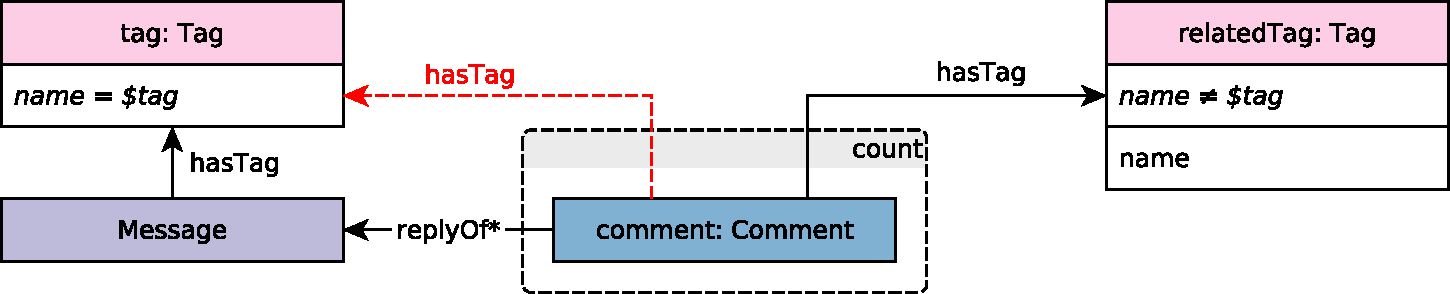
\includegraphics[scale=\patternscale,margin=0cm .2cm]{patterns/bi-read-08}
		\caption{Example graph pattern.}
		\label{fig:example-graph-pattern}
	\end{center}
\end{figure}

\begin{itemize}
	\item Nodes are marked as $\mathsf{entityName: EntityType}$ (camel case 
	notation for both, starting with a lowercase character for the first and an 
	uppercase character for the second). If the $\mathsf{entityName}$ is not used 
	in the query results, aggregations or calculations, and not referenced in the 
	query specification, the $\mathsf{entityName}$ can be omitted.
	\item Positive conditions for edges are denoted with solid lines.
	\item Negative conditions for edges, \ie edges that are not allowed in the graph, are denoted with \textcolor{red}{\dashuline{dashed red}} lines.
	\item Edges without direction imply that there must be an edge in \emph{at least one of the directions}.
	\item Filtering conditions are typeset in \textit{italic}, \eg $\mathit{id} = 
	\mathit{\textdollar tag}$.
	\item Attributes that should be returned are denoted in sans-serif font, \eg $\mathsf{name}$.
	\item Variable length paths, \ie edges that can be traversed multiple times 
	are denoted with $*\mathsf{min}...\mathsf{max}$, \eg $\mathsf{replyOf}*$ or 
	$\mathsf{knows*1 \ldots 2}$. By default, the value of $\mathsf{min}$ is 1, 
	and the value of $\mathsf{max}$ is unlimited.
	\item Aggregations are shown in dashed boxes with the type of aggregation ($\mathsf{count}$, $\mathsf{sum}$, $\mathsf{avg}$, etc.) in the upper right corner.
\end{itemize}

\newcommand{\tuple}[1]{\langle #1 \rangle}

\paragraph{Keywords.} The pattern notation uses a small set of keywords:

\begin{itemize}
	\item $\mathsf{UNWIND}$ unnests a list, \ie produces a set of one-tuples. For 
	example, $\mathsf{UNWIND} [1, 2, 3]$ results in $ \{ \tuple{1}, \tuple{2}, 
	\tuple{3} \} $.
	\item Aggregation operations: \lstinline{count}, \lstinline{avg}. % \lstinline{sum} - sum is not used in the figures as we always sum some derived value
	\item Functions:
	\begin{itemize}
		\item \lstinline{floor(x)} (returns $\lfloor x \rfloor$),
		\item \lstinline{year(date)} (extracts the year from a given date),
		\item \lstinline{month(date)} (extracts the month from a given date).
	\end{itemize}
\end{itemize}

\paragraph{Resolving ambiguity.} Note that if the textual description and the graph pattern are different for a particular query (either due to an error or the lack of sophistication in the graphical syntax), \emph{the textual description takes precedence}.

%%%%%%%%%%%%%%%%%%%%%%%%%%%%%%%%%%%%%%%%%%%%%%%%%%%%%%%%%%%%%%%%%%%%%%%%%%%%%%
%%%%%%%%%%%%%%%%%%%%%%%%%%%%%%%%%%%%%%%%%%%%%%%%%%%%%%%%%%%%%%%%%%%%%%%%%%%%%%
%%%%%%%%%%%%%%%%%%%%%%%%%%%%%%%%%%%%%%%%%%%%%%%%%%%%%%%%%%%%%%%%%%%%%%%%%%%%%%

\section{Substitution Parameters}

Together with the dataset, \datagen produces a set of parameters per
query type. Parameter generation is designed in such a way that for each query
type, all of the generated parameters yield similar runtime behaviour of that
query.

Specifically, the selection of parameters for a query template guarantees the following properties of the resulting queries:
\begin{enumerate}
\item[P1:] the query runtime has a bounded variance: the average runtime corresponds to the behavior of the majority of the queries
\item[P2:] the runtime distribution is stable: different samples of (\eg 10) parameter bindings used in different query streams result in an identical runtime distribution across streams
\item[P3:] the optimal logical plan (optimal operator order) of the queries is the same: this ensures that a specific query template tests the system's behavior under the well-chosen technical difficulty (\eg handling voluminous joins or proper cardinality estimation for subqueries, \etc)
\end{enumerate}


As a result, the amount of data that the query touches is roughly the
same for every parameter binding, assuming that the query optimizer figures out a
reasonable execution plan for the query. This is done to avoid bindings that
cause unexpectedly long or short runtimes of queries, or even result in a
completely different optimal execution plan. Such effects could arise due to
the data skew and correlations between values in the generated dataset.

In order to get the parameter bindings for each of the queries, we have designed a \textit{Parameter Curation} procedure that works in two stages:

\begin{enumerate}
\item for each query template for all possible parameter bindings, we determine the size of intermediate results in the {\em intended} query plan. Intermediate result size heavily influences the runtime of a query, so two queries with the same operator tree and similar intermediate result sizes at every level of this operator tree are expected to have similar runtimes. This analysis is effectively a side effect of data generation, that is we keep all the necessary counts (number of friends per user, number of posts of friends \etc) as we create the dataset.
\item then, a greedy algorithm selects (``curates'') those parameters with similar intermediate result counts from the domain of all the parameters.
\end{enumerate}

Parameter bindings are stored in the \texttt{substitution\_parameters} folder
inside the data generator directory. Each query gets its bindings in a separate
file. Every line of a parameter file is a JSON-formatted collection of
key-value pairs (name of the parameter and its value). For example, the Query 1
parameter bindings are stored in file \texttt{query\_1\_param.txt}, and one of
its lines may look like this:

\vspace{-6mm}
$$
\{\text{"PersonID"}: 1, \text{"Name"}: \text{"Lei"}, \text{"PersonURI"}: \text{"http://www.ldbc.eu/ldbc\_socialnet/1.0/data/pers1"}\}
$$

Depending on implementation, the SUT may refer to persons either by IDs
(relational and graph databases) or URIs (RDF systems), so we provide both
values for the Person parameter.  Finally, parameters for short reads are taken
from those in complex reads and updates.


%%%%%%%%%%%%%%%%%%%%%%%%%%%%%%%%%%%%%%%%%%%%%%%%%%%%%%%%%%%%%%%%%%%%%%%%%%%%%%
%%%%%%%%%%%%%%%%%%%%%%%%%%%%%%%%%%%%%%%%%%%%%%%%%%%%%%%%%%%%%%%%%%%%%%%%%%%%%%
%%%%%%%%%%%%%%%%%%%%%%%%%%%%%%%%%%%%%%%%%%%%%%%%%%%%%%%%%%%%%%%%%%%%%%%%%%%%%%

\section{Load Definition}

\ldbcsnb Test Driver is in charge of the execution of the Interactive Workload.
At the beginning of the execution, the Test Driver creates a query mix by
assigning to each query instance, a query issue time and a set of parameters
taken from the generated substitution parameter set described above.  

Query issue times have to be carefully assigned.  Although substitution
parameters are chosen in such a way that queries of the same type take similar
time, not all query types have the same complexity and touch the same amount of
data, which causes them to scale differently for the different scale factors.
Therefore, if all query instances, regardless of their type, are issued
at the same rate, those more complex queries will dominate the execution's
result, making faster query types purposeless. To avoid this situation, each
query type is executed at a different rate. The way the execution rate is decided,
also depends on the nature of the query: complex read, short read or update.

Update queries' issue times are taken from the update streams generated by the
data generator. These are the times where the actual event happened during the
simulation of the social network. Complex reads' times are expressed in terms
of update operations. For each complex read query type, a frequency value is
assigned which specifies the relation between the number of updates performed
per complex read.  Table~\ref{table:freqs} shows the frequencies assigned to
each query type for SF1. The frequencies of the different scale factors can be
found in Appendix~\ref{appendix:scale_factors}.

\begin{table}[H]
\centering
    \begin{tabular}{|c|c|c|c|}
    \hline
    Query Type & freq & Query Type & freq \\ 
    \hline
    \hline
    Query 1 & 26 & Query 8 & 45 \\ 
    \hline       
    Query 2 & 37 & Query 9 & 157 \\  
    \hline        
    Query 3 & 69 & Query 10 & 30 \\ 
    \hline        
    Query 4 & 36 & Query 11 & 16 \\ 
    \hline        
    Query 5 & 57 & Query 12 & 44 \\ 
    \hline        
    Query 6 & 129 & Query 13 & 19 \\  
    \hline        
    Query 7 & 87 & Query 14 & 49 \\ 
    \hline
    \end{tabular}
    \caption{Frequencies for each query type for SF1.}
    \label{table:freqs}
\end{table}

Finally, short reads are inserted in order to balance the ratio between reads
and writes, and to simulate the behavior of a real user of the social network.
For each complex read instance, a sequence of short reads is planned. There are two
types of short read sequences: Person centric and Message centric. Depending on
the type of the complex read, one of them is chosen. Each sequence consists of
a set of short reads which are issued in a row. The issue time assigned to each
short read in the sequence is determined at run time, and is based on the
completion time of the complex read it depends on. 
The substitution parameters for short reads are taken from the results of previously
executed complex reads and short reads.
Once a short read sequence is issued (and provided that sufficient substitution parameters 
exist), there is a probability that another short read  sequence is issued. 
This probability decreases for each new sequence issued. 
Since the same random number generator seed is used across
executions, the workload is deterministic.


The specified frequencies, implicitly define the query ratios between queries
of different types, as well as a default target throughput. However the Test
Sponsor may specify a different target throughput to test,  by ``squeezing''
together or ``stretching'' apart the queries of the workload. This is
achieved  by means of the ``Time Compression Ratio'' that is multiplied by the
frequencies (see \autoref{table:freqs}).  Therefore, different
throughputs can be tested while maintaining the relative ratios between the
different query types.

%\section{Performance metrics}\label{section:metrics}
\alert{ TODO}
%\alert{ TODO - Renzo \\
%Here we need to describe the different metrics used to evaluate the performance
%of the systems.
%}
%
%\subsection{Response Time}
%
%Response Time (RT) is defined by RT = eT - sT where:
%\begin{itemize}
%    \item sT = time measured before the first byte of input data of the Transaction is sent by the Driver to the SUT;
%    \item eT = time measured after the last byte of output data from the Transaction is received by the Driver from the SUT.
%\end{itemize}
%The resolution of the time stamps used for measuring Response Time is of at least \alert{XX} seconds.
%
%\subsection{Throughput}
%
%The throughput is measured as ''Operations per second at scale'' (\ie opsSI@100).
%The metric is calculated for a run that satisfies the minimum length and per
%query minimum execution count and query mix criteria.
%\alert{Describe here the criteria}
%Each completed operation counts as one operation. The metric is the count of successful operations
%divided by elapsed time in seconds.
%
%\subsection{Interactive Workload Metric}
%
%\alert{Need to elaborate on this. The current description in confluence is incomplete. Is this needed?}
%
%
%\subsection{Price/Performance Metric}
%\alert{We need to include the definition of a price/performance metric.}

%\section{Execution rules}\label{section:rules}

%\subsection{Execution Steps}
%\alert{Some items have to be reviewed}
%A benchmark execution is divided into the following steps:
%\begin{itemize}
%    \item \textbf{Data Preparation.} This includes running the data generator, placing
%        the generated files in a staging area, configuring storage, setting up
%        the SUT configuration and preparing any data partitions in the SUT.
%        This may include pre-allocating database space but may not include
%        loading any data or defining any schema having to do with the
%        benchmark.
%    \item \textbf{Bulk Load.} This includes defining the database schema, if any,
%        loading the initial database population, making this durably stored,
%        gathering any optimizer statistics,.   The bulk load time is reported
%        and is equal to the amount of elapsed wall clock time between starting
%        the schema definition and receiving the confirmation message of the end
%        of statistics gathering.
%    \item \textbf{Benchmark Run.} The run begins after the bulk load or after another
%        benchmark run.  If the run does not directly follow the bulk load, it
%        must start at a point in the update stream that has not previously been
%        played into the database.  In other words, a run may only include
%        update events whose timestamp is later than the latest post creation
%        date in the database prior to start of run.  The run starts when the
%        first of the test drivers sends its first message to the SUT.  If the
%        SUT is in-process with the driver the window starts when the driver
%        starts.
%    \item \textbf{Measurement Window.} The measurement window is the timed portion of
%        the benchmark run. It may begin at any time during the run.  The
%        activity during the measurement window must meet the criteria described in
%        \alert{Section XX}. The measurement window is terminated at
%        the discretion of the test sponsor at any time when the Minimum
%        Measurement Window criteria are met. All the processes constituting
%        the SUT are to be killed at the end of the window or alternatively all
%        the hardware components of the SUT are to be powered off.
%    \item \textbf{Recovery Test.} The SUT is to be restarted after the measurement
%        window and the auditor will verify that the SUT contains the entirety
%        of the last update recorded by the test driver(s) as successfully
%        committed.
%\end{itemize}
%
%\subsection{Rules for the Data Schema}
%
%\ldbcsnb may be implemented with different data models, \eg relational, RDF and
%different graph data models.  The reference schema is provided as RDFS and SQL.
%The data generator produces TTL syntax for RDF and comma separated values for
%other data models. A single attribute has a single data type. The following
%requirements apply:
%
%\begin{itemize}
%    \item \textbf{Identifier:} This is an integer value foreign key or a URI in
%        RDF.  If this is an integer column, the implementation data type should
%        support at least $2^{55}$ distinct values
%    \item \textbf{Datetime:} Should support a date range from 0000 to 9999 in
%        the year field, with a resolution of no less than one second.
%    \item \textbf{String:} A string column for names may have a variable length
%        and may have a declared maximum length, \eg 40 characters.
%    \item \textbf{Long String:} For example a post content may be a long string
%        that is often short in the data but may not declare a maximum length
%        and must support data sizes of up to 1MB \alert{Current generator max post length is set to 2000 characters}..
%\end{itemize}
%
%A single attribute in the reference schema may not be divided into multiple
%attributes in the target schema.
%
%
%A schema on the DBMS is optional.  An RDF implementation for example may work
%without one.  An RDF implementation is allowed to load the RDF reference schema
%and to take advantage of the data type and cardinality statements therein.
%
%
%A relational or graph schema may specify system specific options affecting
%storage layout.  These may for example specify vertical partitioning.  Vertical
%partitioning means anything from a column store layout with per-column
%allocated storage space to use of explicit column groups.  Any mix of row or
%column-wise storage structures is allowed as long as this is declaratively
%specified data structure by data structure.  Data structure here means for
%example table or index.
%
%
%Covering indices and clustered indices are allowed.
%If these are defined, then all replications of data implied by these must be
%maintained statement by statement, \ie each auxiliary data structure must be
%consistent with any other data structures of the table after each data
%manipulation operation.
%
%
%A covering index is an index which materializes a
%specific order of a specific subset or possibly all columns of a table.  A
%clustered index is an index which materializes all columns of a table in a
%specific order, which order may or may not be that of the primary key of the
%table. A clustered or covering index may be the primary or only representation
%of a table.
%
%
%Any subset of the columns on a covering or clustered index may be
%used for ordering the data.  A hash based index or a combination of a hash
%based and tree based index are all allowed, in row or column-wise or hybrid
%forms.
%
%
%\subsection{Rules for Implementing the Workload}
%\subsubsection{Queries' Implementation}
%
%The queries and updates may be implemented in a declarative query language or
%as procedural code using an API.  If a declarative query language is used, \eg
%SPARQL or SQL, then explicit query plans are prohibited in all the read-only
%queries. The update transactions may still consist of multiple statements,
%effectively amounting to explicit plans.
%
%
%Explicit query plans include but \alert{are not limited to (this is too ambiguous and dangerous)}:
%\begin{itemize}
%    \item Directives or hints specifying a join order or join type
%    \item Directives or hints specifying an access path, \eg which index to use
%    \item Directive or hints specifying an expected cardinality, selectivity,
%        fanout or any other information that pertains to the expected number or
%        results or cost of all or part of the query.
%\end{itemize}
%
%\subsubsection{Auxiliary Data Structures and Pre-computation}
%Auxiliary data structures and pre-computations are allowed.  A pre-computation
%may be implemented as client side logic in the test driver, as stored
%procedures or as triggers.  In all cases the operations, whether one or many,
%must constitute a single transaction.  A SPARQL protocol operation consisting
%of multiple statements may be a valid implementation of the if the SUT executes
%the statements as a single transaction. Other pre-computation of query results
%is explicitly prohibited.
%
%\subsubsection{ACID Compliance}
%
%The interactive workload requires full ACID support from the SUT.
%\begin{itemize}
%    \item \textbf{Atomicity.} All the updates in a transaction must either take
%        place or be all cancelled.
%    \item \textbf{Consistency.} If a database object, \eg table, has auxiliary
%        data structures, \eg indices, the content of these must be consistent
%        after the commit or rollback of a transaction.   If multiple client
%        application threads share one transaction context, these may
%        transiently see inconsistent states, \eg there may be a time when an
%       insert of a row is reflected in one index of a table but not in
%        another.
%    \item \textbf{Isolation.} If a transaction reads the database with intent
%        to update, the DBMS must guarantee that repeating the same read within
%        the same transaction will return the same data.  This also means that
%        no more and no less data rows must be returned.  In other words, this
%        corresponds to snapshot or to serializable isolation.  This level of
%        isolation is applied for the operations where the transaction mix so
%        specifies.  If the database is accessed without transaction context or
%        without intent too update, then the DBMS should provide read committed
%        semantics, \eg repeating the same read may produce different results
%        but these results may never include effects of pending uncommitted
%        transactions.
%    \item \textbf{Durability.} The effects of a transaction must be made
%        durable against instantaneous failure before the SUT confirms the
%        successful commit of a transaction to the application. For systems
%        using a transaction log, this implies syncing the durable media of the
%        transaction log before confirming success to the application.  This
%        will typically entail group commit where transactions that fall in the
%        same short window are logged together and the logging device will
%        typically be an SSD or battery backed RAM on a storage controller.  For
%        systems using replication for durability, this will entail receipt of a
%        confirmation message from the replicating party before confirming
%        successful commit to the application.
%\end{itemize}
%
%\subsection{Rules for Running the Test Driver}
%
%A qualifying run must use the \ldbcsnb test driver provided. The test driver
%implements the workload described in \alert{Section XX}.
%The test driver may be modified by the test sponsor for purposes of
%interfacing to the SUT. The parameter generation and result recording and
%workload scheduling parts of the test driver cannot be changed.  The
%auditor needs to have access to the test driver source code used for producing
%the driver used in the reported run.
%
%\alert{ Check whether this is out of date or not}
%
%The test driver is scale-out capable.  Many
%instances of the test driver may be used in a test run.   The number and
%configuration of the test drivers must be disclosed, along with hardware
%details of the platform running the driver(s), together with details of the
%network interface connecting the drivers too the SUT.  The SUT hardware may
%also be used for hosting the driver(s), at the discretion of the test sponsor.
%
%
%A separate test summary tool provided with the test driver analyzes the test
%driver log(s) after a measurement window is completed.  The tool produces for
%each of the distinct queries and transactions the following summary:
%\begin{itemize}
%    \item Count of executions
%    \item Minimum/average/90th percentile/maximum execution time.
%    \item Start and end date of the window in real time and in simulation time.
%    \item Metric in operations per second at scale. (ops) (throughout rating)
%    \item Number of test drivers
%    \item Number of database sessions (threads) per test driver
%\end{itemize}
%
%
%\subsection{Rules for Scaling}
%\ldbcsnb provides predefined scale factors, as described in \alert{Section XX}.
%The validation scale factor is 1.  Official \ldbcsnb results may be published at
%any of the provided scale factors.
%
%
%\subsection{Rules for Checkpointing}
%A checkpoint is defined as the operation which causes data persisted in a
%transaction log to become durable outside of the transaction log. In specific,
%this means that a SUT restart after instantaneous failure following the
%completion of the checkpoint may not have recourse to transaction log entries
%written before the end of the checkpoint.
%
%
%A checkpoint typically involves a
%synchronization barrier at which all data committed prior too the moment is
%required to be in durable storage that does not depend on the transaction log.
%
%
%Not all DBMSs use a checkpointing mechanism for durability. For example a
%system may rely on redundant storage of data for durability guarantees against
%instantaneous failure of a single server.
%
%
%The measurement window may contain a
%checkpoint. If the measurement window does not contain one, then the restart
%test will involve redoing all the updates in the window as part of the recovery
%test.

%\section{Full disclosure}\label{section:disclosure}
\alert{ TODO }
%\alert{ TODO - Peter, Larri and Orri \\
%Here we have to describe what needs to be disclosed to have a valid benchmark report.
%}

%

This chapter describes the rules to audit benchmark runs, that is, what
techniques are allowed and what is not, what must be provided to the auditor
and guidelines for the auditors to perform the audit. 

\section{Preparation}

The first step when doing an audit is to determine the versions of the
following items that will be used for the benchmark:

\begin{itemize}
  \item The Benchmark Specification
  \item The data generator
  \item The driver
\end{itemize}

These must be reported in the full disclosure report to guarantee that the
benchmark run can be reproduced exactly in the future. Similarly, the test
sponsor will inform the auditor the scale factor to test. Finally, a clean test
system with enough space to store the scale factor must be provided, including
the update streams and substitution parameters. 


\subsection{Collect system details}

The next step is to collect the technical and pricing details of the system
under test. This includes the following items:

\begin{itemize}
\item Common name of the system, e.g. Dell PowerEdge xxxx.
\item Type and number of CPU's, cores/threads per CPU, clock frequency and cache hierarchy characteristics (levels, size per level, etc...).
\item The amount of system's memory, type and frequency.
\item The Disk controller or motherborad type if disk controller is on motherboard.
\item For each distinct type of secondary storage device, the number and characteristics of the device.
\item The number and type of network controllers.
\item The number and type of network switches. Wiring must be disclosed.
\item Date of availability of the system.
\end{itemize}

Only the network switches and interfaces that participate in the run need to be
reported. If the benchmark execution is entirely contained on a single machine,
no network need be reported.  The price of the hardware in question must be
disclosed and should reflect the single quantity list price that any buyer
could expect when purchasing one system with the given specification. The price
may be either an item by item price or a package price if the system is sold as
a package

Besides hardware characteristics, also software details must be collected:

\begin{itemize}
\item The DBMS and operating system name and versions.
\item Installation and configuration information of both the DBMS and operating
system, which must be provided by the test sponsor.
\item Price of the software license used, which can be tight to the number of
concurrent users or size of data.
\item Date of availability of the software.
\end{itemize}

Also, the test sponsor must provide all the source code relevant to the
benchmark.

\subsection{Setup the benchmark environment}

Once all the information has been collected, the auditor will setup the
environment to perform the benchmark run. This setup includes configuring the
following items:


\begin{itemize}
\item Setup the LDBC Data generator in the test machine if datasets are not
available from a trusted source.
\item Setup the LDBC driver with the connectors provided by the test sponsor.
The test sponsor must provide the configuration parameters to configure the
driver (tcr, number of threads, etc.).  ldbc.snb.interactive.update\_interleave
driver parameter must come from the updateStream.properties file, which is
created by the data generator.That parameter should never be set manually.
Also, make sure that the -rl/--results\_log is enabled.  Make sure that all
operations are enabled and the frequencies are those for the selected scale
factor. These can found in Appendix\ref{appendix:scale_factors}.  If the driver
will be executed on a separate machine, gather the characteristics of that
machine in the same way as specified above.
\end{itemize}


\subsection{Load data}

The test sponsor must provide all the necessary documentation and scripts
to load the dataset into the database to test. The system under test must
support the different data types needed by the benchmark for each of the
attributes at their needed precision. No data can be filtered out, everything
must be loaded.  The test sponsor must provide a tool to perform arbitrary
checks of the data or a shell to issue queries in a declarative language if the
system supports it. The auditor will measure the time to load the data, which
will be disclosed.

\section{Running the benchmark}

Running the benchmark consists of three separate parts: validating the query
implementations, warming the database and performing the benchmark run. The
queries are validated by means of the official validation datasets provided by
LDBC consortium in their official software repositories. The auditor must load
the provided dataset and run the driver in validation mode, which will test
that the queries provide the official results.


The warmup can be performed either using the LDBC driver or externally, and the
way it is performed must be disclosed.

A valid benchmark run must last at least 2 hours of simulation time (datagen
time).  Also, in order to be valid, a benchmark run needs to meet the following
requirements.  Results\_log.csv contains the actual\_start\_time and
scheduled\_start\_time of each of the issued queries.  In order to have a valid
run, 95\% of the queries must meet the following condition: 

\begin{equation*}
actual\_start\_time - scheduled\_start\_time < 1 \ second
\end{equation*}

If the execution of the benchmark is valid, the auditor must retrieve all the
files from directory specified by -rd/--results\_dir which includes
configuration settings used, results log, results summary, which will be
disclosed.

\section{Recovery}

Once an official run has been validated, the recovery capabilities of the
systemm must be tested. The system and the driver must be configured in the
same way as in during the benchmark execution. The system will be warmup and an
execution of the benchmark will be performed under the same terms as in the
previous measured run.

At an arbitrary point after 2 hours of simulation time execution, the machine
will be disconnected.  Then, the auditor will restart the database system and
will check that the last commited update (in the driver log file) is actually
in the database. The auditor will measure the time taken by the system to
recover from the failure. Also, all the information about how durability is 
ensured must be disclosed. If checkpoints are used, these must be performed 
with a period of 10 minutes at most.


\section{Serializability}

Optionally, the test sponsor can execute update queries atomically. The auditor
will verify that serializability is guaranteed. 





%%%%%%%%%%%%%%%%%%%%%%%%%%%%%%%%%%%%%%%%%%%%%%%%%%%%%%%%%%%%%%%%%%%%%%%%%%%%%%
%%%%%%%%%%%%%%%%%%%%%%%%%%%%%%%%%%%%%%%%%%%%%%%%%%%%%%%%%%%%%%%%%%%%%%%%%%%%%%
%%%%%%%%%%%%%%%%%%%%%%%%%%%%%%%%%%%%%%%%%%%%%%%%%%%%%%%%%%%%%%%%%%%%%%%%%%%%%%



\chapter{Auditing rules}\label{chapter:auditing}


This chapter describes the rules to audit benchmark runs, that is, what
techniques are allowed and what is not, what must be provided to the auditor
and guidelines for the auditors to perform the audit. 

\section{Preparation}

The first step when doing an audit is to determine the versions of the
following items that will be used for the benchmark:

\begin{itemize}
  \item The Benchmark Specification
  \item The data generator
  \item The driver
\end{itemize}

These must be reported in the full disclosure report to guarantee that the
benchmark run can be reproduced exactly in the future. Similarly, the test
sponsor will inform the auditor the scale factor to test. Finally, a clean test
system with enough space to store the scale factor must be provided, including
the update streams and substitution parameters. 


\subsection{Collect system details}

The next step is to collect the technical and pricing details of the system
under test. This includes the following items:

\begin{itemize}
\item Common name of the system, e.g. Dell PowerEdge xxxx.
\item Type and number of CPU's, cores/threads per CPU, clock frequency and cache hierarchy characteristics (levels, size per level, etc...).
\item The amount of system's memory, type and frequency.
\item The Disk controller or motherborad type if disk controller is on motherboard.
\item For each distinct type of secondary storage device, the number and characteristics of the device.
\item The number and type of network controllers.
\item The number and type of network switches. Wiring must be disclosed.
\item Date of availability of the system.
\end{itemize}

Only the network switches and interfaces that participate in the run need to be
reported. If the benchmark execution is entirely contained on a single machine,
no network need be reported.  The price of the hardware in question must be
disclosed and should reflect the single quantity list price that any buyer
could expect when purchasing one system with the given specification. The price
may be either an item by item price or a package price if the system is sold as
a package

Besides hardware characteristics, also software details must be collected:

\begin{itemize}
\item The DBMS and operating system name and versions.
\item Installation and configuration information of both the DBMS and operating
system, which must be provided by the test sponsor.
\item Price of the software license used, which can be tight to the number of
concurrent users or size of data.
\item Date of availability of the software.
\end{itemize}

Also, the test sponsor must provide all the source code relevant to the
benchmark.

\subsection{Setup the benchmark environment}

Once all the information has been collected, the auditor will setup the
environment to perform the benchmark run. This setup includes configuring the
following items:


\begin{itemize}
\item Setup the LDBC Data generator in the test machine if datasets are not
available from a trusted source.
\item Setup the LDBC driver with the connectors provided by the test sponsor.
The test sponsor must provide the configuration parameters to configure the
driver (tcr, number of threads, etc.).  ldbc.snb.interactive.update\_interleave
driver parameter must come from the updateStream.properties file, which is
created by the data generator.That parameter should never be set manually.
Also, make sure that the -rl/--results\_log is enabled.  Make sure that all
operations are enabled and the frequencies are those for the selected scale
factor. These can found in Appendix\ref{appendix:scale_factors}.  If the driver
will be executed on a separate machine, gather the characteristics of that
machine in the same way as specified above.
\end{itemize}


\subsection{Load data}

The test sponsor must provide all the necessary documentation and scripts
to load the dataset into the database to test. The system under test must
support the different data types needed by the benchmark for each of the
attributes at their needed precision. No data can be filtered out, everything
must be loaded.  The test sponsor must provide a tool to perform arbitrary
checks of the data or a shell to issue queries in a declarative language if the
system supports it. The auditor will measure the time to load the data, which
will be disclosed.

\section{Running the benchmark}

Running the benchmark consists of three separate parts: validating the query
implementations, warming the database and performing the benchmark run. The
queries are validated by means of the official validation datasets provided by
LDBC consortium in their official software repositories. The auditor must load
the provided dataset and run the driver in validation mode, which will test
that the queries provide the official results.


The warmup can be performed either using the LDBC driver or externally, and the
way it is performed must be disclosed.

A valid benchmark run must last at least 2 hours of simulation time (datagen
time).  Also, in order to be valid, a benchmark run needs to meet the following
requirements.  Results\_log.csv contains the actual\_start\_time and
scheduled\_start\_time of each of the issued queries.  In order to have a valid
run, 95\% of the queries must meet the following condition: 

\begin{equation*}
actual\_start\_time - scheduled\_start\_time < 1 \ second
\end{equation*}

If the execution of the benchmark is valid, the auditor must retrieve all the
files from directory specified by -rd/--results\_dir which includes
configuration settings used, results log, results summary, which will be
disclosed.

\section{Recovery}

Once an official run has been validated, the recovery capabilities of the
systemm must be tested. The system and the driver must be configured in the
same way as in during the benchmark execution. The system will be warmup and an
execution of the benchmark will be performed under the same terms as in the
previous measured run.

At an arbitrary point after 2 hours of simulation time execution, the machine
will be disconnected.  Then, the auditor will restart the database system and
will check that the last commited update (in the driver log file) is actually
in the database. The auditor will measure the time taken by the system to
recover from the failure. Also, all the information about how durability is 
ensured must be disclosed. If checkpoints are used, these must be performed 
with a period of 10 minutes at most.


\section{Serializability}

Optionally, the test sponsor can execute update queries atomically. The auditor
will verify that serializability is guaranteed. 



\chapter{Implementation Instructions}\label{chapter:instructions}
%%% INSTRUCTIONS %%%

%%%%%%%%%%%%%%%%%%%%%%%%%%%%%%%%%%%%%%%%%%%%%%%%%%%%%%%%%%%%%%%%%%%%%%%%%%%%%%
%%%%%%%%%%%%%%%%%%%%%%%%%%%%%%%%%%%%%%%%%%%%%%%%%%%%%%%%%%%%%%%%%%%%%%%%%%%%%%
%%%%%%%%%%%%%%%%%%%%%%%%%%%%%%%%%%%%%%%%%%%%%%%%%%%%%%%%%%%%%%%%%%%%%%%%%%%%%%

\section{Data generation}
\label{section:data_generation}

\datagen uses Hadoop to implement the data generation. Detailed instructions
to configure hadoop for running \datagen can be found at the DATAGEN project
software repository\footnote{ \datagen repository:
https://github.com/ldbc/ldbc\_snb\_datagen}. 

\subsection{\datagen Configuration, Compilation and Execution}

\datagen is designed to be as easy to configure, compile and execute as
possible. With this objective in mind, a \textit{run.sh} script is provided,
which handles all the compilation and execution processes.  \textit{run.sh}
is found in the \datagen root folder. DATAGEN uses Apache Maven to download any
required dependencies and compile the sources.  \textit{run.sh} needs to be
configured with two variables pointing to the proper folders. The following is
the list of variables to set:

\begin{itemize}
    \item \textbf{HADOOP\_HOME}: Points to your hadoop root folder.
    \item \textbf{LDBC\_SNB\_\datagen\_HOME}: Points to your DATAGEN root folder.
\end{itemize}

Once these variables are properly set, by typing:

\begin{lstlisting}[backgroundcolor=\color{gray}, frame=single, language=bash]
$ ./run.sh
\end{lstlisting}

\datagen is compiled and executed, and a dataset with the default options is
generated in the current folder.

A file \textit{params.ini} is used to change the characteristics of the
generated network, as well as to set other options. \autoref{table:sndg_options}
summarizes the different available options and their default values:

\begin{table}[h]
\centering
\begin{tabular}{|p{2.5cm}|p{2.5cm}|p{10.5cm}|}
    \hline
    \textbf{Option} & \textbf{Default} & \textbf{Description} \\
    \hline
    scaleFactor & 1 & The scale factor of the data to generate. Possible values are: 1, 3, 10, 30, 100, 300 and 1000 \\
    \hline
    serializer & csv & The format of the output data. Options are: csv, csv\_merge\_foreign, ttl \\
    \hline
    compressed & false & Specifies to compress the output data in gzip. \\
    \hline
    outputDir & ./ & Specifies the folder to output the data. \\
    \hline
    numThreads & 1 & Sets the number of threads to use. Only works for pseudo-distributed mode \\
    \hline
    updateStreams & false & Sets \datagen to generate the update streams used by the driver to issue update queries. \\
    \hline
    numUpdatePartitions & 1 & The number of update stream partitions per thread. \\
    \hline
\end{tabular}
\caption{Description of the data types.}
\label{table:sndg_options}
\end{table}

An example of \textit{params.ini} for scale factor 30, ttl serializer, 4 threads,
compressed output and a custom output dir, should look like:

\begin{lstlisting}[backgroundcolor=\color{gray},frame=single]
scaleFactor:30
serializer:ttl
compressed:true
outputDir:/home/user/output
numThreads:4
\end{lstlisting}

\datagen outputs data into HDFS. The outputDir directory specified in
\textit{params.ini} file, will be automatically created in HDFS if it does not
exist. If there is not an HDFS file system mounted, then data is output to your
local file system. 

\datagen creates two directories in the \textit{outputDir} directory: hadoop and
social\_network.  The former is used to store temporary files used during the
data generation process. The later stores the actual dataset created in the
specified format.

Additionally, \datagen creates a third directory in the DATAGEN home folder
called \textit{substitution\_parameters}.  This folder contains the files with
the substitution parameters used by the driver to execute the workload.



\section{Running the benchmark}

Running a benchmark workload involves a number of steps, including data import, driver configuration and workload execution.
The data import step involves loading the output of the data generator into the vendor database,
deploying the database and, optionally, performing a warm-up phase.
The other steps are explained in the following sections.

\subsection{Driver Configuration}
\label{sub:driver_configuration}

Before running a benchmark workload the workload driver~\cite{test_driver} must be configured, this involves the following steps:
\begin{enumerate}
	\item Programming: implement a vendor specific database connector (covered in section \ref{ssub:vendor_specific_database_connector})
	\item Configuration: configure the general driver properties (covered in section \ref{ssub:general_driver_properties})
	\item Configuration: configure the workload specific driver properties (covered in \ref{ssub:workload_specific_driver_properties})
\end{enumerate}

\subsubsection{Vendor specific database connector}
\label{ssub:vendor_specific_database_connector}
Vendors must provide the workload driver with implementations for a number of Java classes: \texttt{Db} and \texttt{OperationHandler}.
More specifically, one implementation of \texttt{Db},
(optionally) one implementation of \texttt{DbConnectionState} (used to manage shared resources among queries, \eg network connections),
and one implementation of \texttt{OperationHandler} per query in the workload.

As a guide, to implement the necessary classes for a workload of two queries (\texttt{LdbcQuery1} and \texttt{LdbcQuery2}),
see the code snippet below.
For a more detailed explanation of how this is done refer to the workload driver documentation \cite{test_driver}.

{\footnotesize
	\begin{verbatim}
    public class ExampleDbConnectionState extends DbConnectionState {
        private Client client;
        public ExampleDbConnectionState(String url){
            client = new Client(url);
        }

        public getClient(){
            return client;
        }
    }

    public class ExampleDb extends Db {
        private ExampleDbConnectionState state;

        @Override
        protected void onInit(Map<String, String> properties) throws DbException {
            registerOperationHandler(LdbcQuery1.class, LdbcQuery1Handler.class);
            registerOperationHandler(LdbcQuery2.class, LdbcQuery2Handler.class);
            state = new ExampleDbConnectionState(properties.get(``url''));
        }

        @Override
        protected void onCleanup() throws DbException {}

        @Override
        protected DbConnectionState getConnectionState() throws DbException {
            return state;
        }

        public static class LdbcQuery1Handler extends OperationHandler<LdbcQuery1> {
            @Override
            protected OperationResult executeOperation(LdbcQuery1 operation) throws DbException {
                Client client = ((ExampleDbConnectionState)dbConnectionState()).getClient();
                LdbcQuery1Result result = client.execute(operation)
                int resultCode = // typically used for debugging, \eg to return error codes
                return operation.buildResult(resultCode, result);
            }
        }

        public static class LdbcQuery2ToHandler extends OperationHandler<LdbcQuery2> {
            @Override
            protected OperationResult executeOperation(LdbcQuery2 operation) throws DbException {
                Client client = ((ExampleDbConnectionState)dbConnectionState()).getClient();
                LdbcQuery2Result result = client.execute(operation)
                int resultCode = // typically used for debugging, \eg returning error codes
                return operation.buildResult(resultCode, result);
            }
        }
    }
	\end{verbatim}
}

\subsubsection{General driver properties}
\label{ssub:general_driver_properties}
Although a detailed explanation of the workload driver design is beyond the
scope of this document, it is worth noting that it has a number of
configuration parameters, these parameters are summarized in
\tref{tab:general_driver_parameters}.

\begin{table}[h!]
	\label{tab:general_driver_parameters}
	\begin{center}
		\begin{tabular}{|l|l|l|}
		\hline
		status 					& boolean & intermittently output workload status during execution \\
		\hline
		operationcount 			& integer & number of queries to generate \\
		\hline
		threadcount 			& integer & size of thread pool to use for query execution \\
		\hline
		resultfile 				& string & path to where workload results will be written \\
		\hline
		timeunit 				& enum & time unit to report result metrics in \\
		\hline
		timecompressionratio 	& double & adjust all query start times proportionally \\
		\hline
		gctdeltaduration 		& integer & min duration (ms) between dependent reads and writes \\
		\hline
		peeridentifiers 		& string[] & addresses of other driver processes (for distributed mode) \\
		\hline
		toleratedexecutiondelay & integer & max allowed time between scheduled and actual query start times \\
		\hline
		workload 				& string & class name of specific \texttt{Workload} implementation \\
		\hline
		database 				& string & class name of specific \texttt{Db} implementation \\
		\hline
		\end{tabular}
	\end{center}
	\caption{General Driver Parameters}
\end{table}
Note that default configuration files, with relevant parameter values set and required parameters commented,
are provided in the driver distribution.

\subsubsection{Workload specific driver properties}
\label{ssub:workload_specific_driver_properties}

In addition to the general driver properties, the driver supports the definition of arbitrary properties,
which are passed along to the pluggable driver components: \texttt{Db} and \texttt{Workload}.
The first, \texttt{Db}, was described already in the previous section.
The second is \texttt{Workload}, it is the class responsible for defining which operations, in which order and at what throughput, the driver will generate.
From the point of view of the driver, the LDBC Social Network Benchmark is an implementation of the \texttt{Workload} class,
in this case named \texttt{LdbcInteractiveWorkload}.
For more details regarding the workload itself see \ref{section:workload}.

The configuration parameters for the \texttt{LdbcInteractiveWorkload} workload are summarized in \tref{tab:snb_interactive_driver_parameters}.

\begin{table}[h!]
	\label{tab:snb_interactive_driver_parameters}
	\begin{center}
		\begin{tabular}{|l|l|l|}
		\hline
		parameter\_dir &
		string &
		data generator parameters directory (read parameters) \\
		\hline
		data\_dir &
		string &
		data generator data directory (dataset and write parameters) \\
		\hline
		LdbcQuery1\_interleave &
		boolean &
		interval between successive query 1 executions\\
		\hline
		LdbcQuery2\_interleave &
		boolean &
		interval between successive query 2 executions\\
		\hline
		LdbcQuery3\_interleave &
		boolean &
		interval between successive query 3 executions\\
		\hline
		LdbcQuery4\_interleave &
		boolean &
		interval between successive query 4 executions\\
		\hline
		LdbcQuery5\_interleave &
		boolean &
		interval between successive query 5 executions\\
		\hline
		LdbcQuery6\_interleave &
		boolean &
		interval between successive query 6 executions\\
		\hline
		LdbcQuery7\_interleave &
		boolean &
		interval between successive query 7 executions\\
		\hline
		LdbcQuery8\_interleave &
		boolean &
		interval between successive query 8 executions\\
		\hline
		LdbcQuery9\_interleave &
		boolean &
		interval between successive query 9 executions\\
		\hline
		LdbcQuery10\_interleave &
		boolean &
		interval between successive query 10 executions\\
		\hline
		LdbcQuery11\_interleave &
		boolean &
		interval between successive query 11 executions\\
		\hline
		LdbcQuery12\_interleave &
		boolean &
		interval between successive query 12 executions\\
		\hline
		LdbcQuery13\_interleave &
		boolean &
		interval between successive query 13 executions\\
		\hline
		LdbcQuery14\_interleave &
		integer &
		interval between successive query 14 executions\\
		\hline
		LdbcQuery1\_enable &
		boolean &
		enable/disable read query 1 \\
		\hline
		LdbcQuery2\_enable &
		boolean &
		enable/disable read query 2 \\
		\hline
		LdbcQuery3\_enable &
		boolean &
		enable/disable read query 3 \\
		\hline
		LdbcQuery4\_enable &
		boolean &
		enable/disable read query 4 \\
		\hline
		LdbcQuery5\_enable &
		boolean &
		enable/disable read query 5 \\
		\hline
		LdbcQuery6\_enable &
		boolean &
		enable/disable read query 6 \\
		\hline
		LdbcQuery7\_enable &
		boolean &
		enable/disable read query 7 \\
		\hline
		LdbcQuery8\_enable &
		boolean &
		enable/disable read query 8 \\
		\hline
		LdbcQuery9\_enable &
		boolean &
		enable/disable read query 9 \\
		\hline
		LdbcQuery10\_enable &
		boolean &
		enable/disable read query 10 \\
		\hline
		LdbcQuery11\_enable &
		boolean &
		enable/disable read query 11 \\
		\hline
		LdbcQuery12\_enable &
		boolean &
		enable/disable read query 12 \\
		\hline
		LdbcQuery13\_enable &
		boolean &
		enable/disable read query 13 \\
		\hline
		LdbcQuery14\_enable &
		boolean &
		enable/disable read query 14 \\
		\hline
		LdbcUpdate1AddPerson\_enable &
		boolean &
		enable/disable update query 1 \\
		\hline
		LdbcUpdate2AddPostLike\_enable &
		boolean &
		enable/disable update query 2 \\
		\hline
		LdbcUpdate3AddCommentLike\_enable &
		boolean &
		enable/disable update query 3 \\
		\hline
		LdbcUpdate4AddForum\_enable &
		boolean &
		enable/disable update query 4 \\
		\hline
		LdbcUpdate5AddForumMembership\_enable &
		boolean &
		enable/disable update query 5 \\
		\hline
		LdbcUpdate6AddPost\_enablet &
		boolean &
		enable/disable update query 6 \\
		\hline
		LdbcUpdate7AddComment\_enable &
		boolean &
		enable/disable update query 7 \\
		\hline
		LdbcUpdate8AddFriendship\_enable &
		boolean &
		enable/disable update query 8 \\
		\hline
		\end{tabular}
	\end{center}
	\caption{LDBC Social Network Benchmark Parameters}
\end{table}

\subsection{Running Workload}
\label{sub:running_workload}

Finally, to run the workload execute the \texttt{main} method of the \texttt{Client} class in the driver.
The general pattern for doing so is as follows:

{\footnotesize
	\begin{verbatim}
	usage: java -cp core-VERSION.jar com.ldbc.driver.Client [-db <classname>] [-del <duration>] [-gctd <duration>]
	       [-oc <count>] [-P <file1:file2>] [-p <key=value>] [-pids <peerId1:peerId2>] [-rf <path>] [-s] [-tc
	       <count>] [-tcr <ratio>] [-tu <unit>] [-w <classname>]
	   -db,--database <classname>                    classname of the DB to use (e.g.
	                                                 com.ldbc.driver.workloads.simple.db.BasicDb)
	   -del,--toleratedexecutiondelay <duration>     duration (ms) an operation handler may miss its scheduled
	                                                 start time by
	   -gctd,--gctdeltaduration <duration>           safe duration (ms) between dependent operations
	   -oc,--operationcount <count>                  number of operations to execute (default: 0)
	   -P <file1:file2>                              load properties from file(s) - files will be loaded in the
	                                                 order provided
	                                                 first files are highest priority; later values will not
	                                                 override earlier values
	   -p <key=value>                                properties to be passed to DB and Workload - these will
	                                                 override properties loaded from files
	   -pids,--peeridentifiers <peerId1:peerId2>     identifiers/addresses of other driver workers (for
	                                                 distributed mode)
	   -rf,--resultfile <path>                       where benchmark results JSON file will be written (null =
	                                                 file will not be created)
	   -s,--status                                   show status during run
	   -tc,--threadcount <count>                     number of worker threads to execute with (default: 2)
	   -tcr,--timecompressionratio <ratio>           change duration between operations of workload
	   -tu,--timeunit <unit>                         time unit to use when gathering metrics.
	                                                 default:MILLISECONDS, valid:[NANOSECONDS, MICROSECONDS,
	                                                 MILLISECONDS, SECONDS, MINUTES]
	   -w,--workload <classname>                     classname of the Workload to use (e.g.
	                                                 com.ldbc.driver.workloads.simple.SimpleWorkload)
	\end{verbatim}
}

For the Interactive workload of LDBC-SNB it is necessary to provide the driver with four configuration files, containing:
general driver properties,
workload specific driver properties (\eg database connection string),
a dataset specific value for one of the general driver properties (specifically, \texttt{gctdeltaduration}),
and vendor specific database properties.
The commandline to execute the workload would look something like:

{\footnotesize
	\begin{verbatim}
	java -cp ldbc_driver/target/core-0.2-SNAPSHOT.jar com.ldbc.driver.Client
		-db com.vendor.VendorDb
		-P vendor/vendor.properties,
		-P data_generator/outputDir/updateStream_0.properties,
		-P ldbc_driver/workloads/ldbc/socnet/interactive/ldbc_socnet_interactive.properties
		-P ldbc_driver/src/main/resources/ldbc_driver_default.properties
	\end{verbatim}
}


\section{ Gathering the results }

Gathering the results for a benchmark run is a simple matter of referring to the results JSON file emitted by the driver.
The format of that file is as follows:

{\footnotesize
	\begin{verbatim}
	{
	  "unit": "MILLISECONDS",
	  "start_time": 1400750662691,
	  "finish_time": 1400750667691,
	  "total_duration": 5000,
	  "total_count": 50,
	  "all_metrics": [
	    {
	      "name": "Query1",
	      "count": 50,
	      "unit": "MILLISECONDS",
	      "run_time": {
	        "name": "Runtime",
	        "unit": "MILLISECONDS",
	        "count": 50,
	        "mean": 100,
	        "min": 2,
	        "max": 450,
	        "50th_percentile": 98,
	        "90th_percentile": 129,
	        "95th_percentile": 432,
	        "99th_percentile": 444
	      },
	      "start_time_delay": {
	        "name": "Start Time Delay",
	        "unit": "MILLISECONDS",
	        "count": 7,
	        "mean": 3.5714285714285716,
	        "min": 0,
	        "max": 25,
	        "50th_percentile": 0,
	        "90th_percentile": 0,
	        "95th_percentile": 25,
	        "99th_percentile": 25
	      },
	      "result_code": {
	        "name": "Result Code",
	        "unit": "Result Code",
	        "count": 50,
	        "all_values": {
	          "0": 42,
	          "1": 8
	        }
	      }
	    }
	  ]
	}
	\end{verbatim}
}

\section{Validation}

LDBC-SNB driver provides a validation mechanism to test the correctness of a benchmark 
workload implementation. To use it, one must provide a validation dataset, which contains
the following items:
\begin{itemize}
    \item a set of substituion parameters;
    \item a set of expected results;
    \item the dataset;
    \item a driver configuration file.
\end{itemize}

Validation datasets are provided by LDBC-SNB, and can be found in the official github 
LDBC repository. 
Once the vendor has implemented the workload, it must load the provided dataset and run
the benchmark with the ``validatedatabase'' option set. With this option, the
driver will read the file with the expected results, and compare them with the results
obtained by the vendor. For more information visit the ldbc driver page.



\bibliographystyle{plain}
\bibliography{references}

\appendix

\chapter{Interactive Query Set Implementations}

\section{Virtuoso SPARQL 1.1}

\subsection{Query 1} 
{\footnotesize
\begin{verbatim}
 sparql select ?fr ?last min(?dist) as ?mindist  ?bday ?since ?gen ?browser ?locationIP 
    ((select group_concat (?email, ", ")
        where {
            ?frr snvoc:email ?email .
            filter (?frr = ?fr) .
        }
        group by ?frr)) as ?email
    ((select group_concat (?lng, ", ")
        where {
            ?frr snvoc:speaks ?lng .
            filter (?frr = ?fr) .
        }
        group by ?frr)) as ?lng
    ?based
    ((select group_concat ( bif:concat (?o_name, " ", ?year, " ", ?o_country), ", ")
        where {
        ?frr snvoc:studyAt ?w .
        ?w snvoc:classYear ?year .
            ?w snvoc:hasOrganisation ?org .
            ?org snvoc:isLocatedIn ?o_countryURI .
        ?o_countryURI foaf:name ?o_country .
            ?org foaf:name ?o_name .
        filter (?frr = ?fr) .
        }
        group by ?frr)) as ?studyAt
    ((select group_concat ( bif:concat (?o_name, " ", ?year, " ", ?o_country), ", ")
        where {
            ?frr snvoc:workAt ?w .
            ?w snvoc:workFrom ?year .
            ?w snvoc:hasOrganisation ?org .
            ?org snvoc:isLocatedIn ?o_countryURI .
            ?o_countryURI foaf:name ?o_country .
            ?org foaf:name ?o_name .
            filter (?frr = ?fr) .
        }
        group by ?frr)) as ?workAt
    {
        ?fr a snvoc:Person .
        ?fr snvoc:firstName "%Name%" .
        ?fr snvoc:lastName ?last .
        ?fr snvoc:birthday ?bday .
        ?fr snvoc:isLocatedIn ?basedURI .
        ?basedURI foaf:name ?based .
        ?fr snvoc:creationDate ?since .
        ?fr snvoc:gender ?gen .
        ?fr snvoc:locationIP ?locationIP .
        ?fr snvoc:browserUsed ?browser .

        {
          { select distinct ?fr (1 as ?dist)
            where {
              sn:pers%Person% snvoc:knows ?fr.
            }
          }
      union
          { select distinct ?fr (2 as ?dist)
            where {
              sn:pers%Person% snvoc:knows ?fr2. 
                              ?fr2 snvoc:knows ?fr.
                              filter (?fr != sn:pers%Person%).
            }
          }
      union
          { select distinct ?fr (3 as ?dist)
            where {
              sn:pers%Person% snvoc:knows ?fr2. 
                              ?fr2 snvoc:knows ?fr3. 
                              ?fr3 snvoc:knows ?fr. 
                              filter (?fr != sn:pers%Person%).
            }
          } .
        }
    }
    group by ?fr ?last ?bday ?since ?gen ?browser ?locationIP ?based
    order by ?mindist ?last ?fr
    limit 20
\end{verbatim}
}
 

\subsection{Query 2}

{\footnotesize
\begin{verbatim}
 sparql select ?fr ?first ?last ?post ?content ?date 
from <sib>
where {
  sn:pers%Person% snvoc:knows ?fr.
  ?fr snvoc:firstName ?first. ?fr snvoc:lastName ?last .
  ?post snvoc:hasCreator ?fr.
  { {?post snvoc:content ?content } union { ?post snvoc:imageFile ?content }} .
  ?post snvoc:creationDate ?date.
  filter (?date <= "%Date0%"^^xsd:date).
}
order by desc (?date) ?post
limit 20
\end{verbatim}
}


\subsection{Query 3}

{\footnotesize
\begin{verbatim}
 sparql select ?fr ?first ?last ?ct1 ?ct2 (?ct1 + ?ct2) as ?sum 
from <sib>  
where { 
    {select distinct ?fr ?first ?last
        (((select count (*)
        where {
            ?post snvoc:hasCreator ?fr .
            ?post snvoc:creationDate ?date .
            filter (?date >= "%Date0%"^^xsd:date && 
                    ?date < bif:dateadd ("day", %Duration%, "%Date0%"^^xsd:date)) .
            ?post snvoc:isLocatedIn dbpedia:%Country1%
        }))
        as ?ct1)
        ((select count (*)
        where {
            ?post2 snvoc:hasCreator ?fr .
            ?post2 snvoc:creationDate ?date2 . 
            filter (?date2 >= "%Date0%"^^xsd:date && 
                    ?date2 < bif:dateadd ("day", %Duration%, "%Date0%"^^xsd:date)) .
            ?post2 snvoc:isLocatedIn dbpedia:%Country2%
        })
        as ?ct2)
    where {
        {sn:pers%Person% snvoc:knows ?fr.} union { sn:pers%Person% snvoc:knows ?fr2.
                                                    ?fr2 snvoc:knows ?fr.
                                                    filter (?fr != sn:pers%Person%)
                                                }.
        ?fr snvoc:firstName ?first . ?fr snvoc:lastName ?last .
        ?fr snvoc:isLocatedIn ?city .
    filter(!exists {?city snvoc:isPartOf dbpedia:%Country1%}).
    filter(!exists {?city snvoc:isPartOf dbpedia:%Country2%}).
    }
    }.
    filter (?ct1 > 0 && ?ct2 > 0) .
}
order by desc(6) ?fr
limit 20
\end{verbatim}
}

 

\subsection{Query 4}
{\footnotesize
\begin{verbatim}
sparql select ?tagname count (*) #Q4
from <sib>
where {
    ?post a snvoc:Post .
    ?post snvoc:hasCreator ?fr .
    ?post snvoc:hasTag ?tag .
    ?tag foaf:name ?tagname .
    ?post snvoc:creationDate ?date . 
    sn:pers%Person% snvoc:knows ?fr .
    filter (?date >= "%Date0%"^^xsd:date && 
            ?date <= bif:dateadd ("day", %Duration%, "%Date0%"^^xsd:date) ) .
    filter (!exists {
        sn:pers%Person% snvoc:knows ?fr2 .
        ?post2 snvoc:hasCreator ?fr2 .
        ?post2 snvoc:hasTag ?tag .
        ?post2 snvoc:creationDate ?date2 .
        filter (?date2 < "%Date0%"^^xsd:date)}) 
    }
group by ?tagname
order by desc(2) ?tagname
limit 10
\end{verbatim}
}


\subsection{Query 5}
{\footnotesize
\begin{verbatim}
sparql select ?title count (*) #Q5
from <sib>
where {
    {select distinct ?fr
        from <sib>
        where {
            {sn:pers%Person% snvoc:knows ?fr.} 
            union {sn:pers%Person% snvoc:knows ?fr2. 
                   ?fr2 snvoc:knows ?fr. 
                   filter (?fr != sn:pers%Person%)}
        }
    } .
    ?group snvoc:hasMember ?mem .
    ?mem snvoc:hasPerson ?fr .
    ?mem snvoc:joinDate ?date .
    filter (?date >= "%Date0%"^^xsd:date) .
    ?post snvoc:hasCreator ?fr .
    ?group snvoc:containerOf ?post .
    ?group snvoc:title ?title.
}
group by ?title
order by desc(2) ?title
limit 20
\end{verbatim}
}
 

\subsection{Query 6}
{\footnotesize
\begin{verbatim}
sparql select ?tagname count (*) 
from <sib>
where {  
    {  select distinct ?fr
       from <sib>
       where {
           {sn:pers%Person% snvoc:knows ?fr.} union { sn:pers%Person% snvoc:knows ?fr2.
                                                      ?fr2 snvoc:knows ?fr.
                                                      filter (?fr != sn:pers%Person%) }
       }
    } .
    ?post snvoc:hasCreator ?fr .
    ?post snvoc:hasTag ?tag1 .
    ?tag1 foaf:name ?tagname1 .
    filter (?tagname1 != '%Tag%') .
    ?post snvoc:hasTag ?tag .
    ?tag foaf:name ?tagname .
}
group by ?tagname
order by desc(2) ?tagname
limit 10
\end{verbatim}
}




\subsection{Query 7}
{\footnotesize
\begin{verbatim}
 sparql select ?liker ?first ?last ?ldt 
       (if ((exists {  sn:pers%Person% snvoc:knows ?liker}), 0, 1) as ?is_new)
       ?post ?content (bif:datediff ("minute", ?dt, ?ldt) as ?lag) 
from <sib>
where {
  ?post snvoc:hasCreator sn:pers%Person% .
  {{ ?post snvoc:content ?content } union {?post snvoc:imageFile ?content}} .
  ?lk snvoc:hasPost ?post .
  ?liker snvoc:likes ?lk . ?liker  snvoc:firstName ?first . ?liker snvoc:lastName ?last . 
  ?post snvoc:creationDate ?dt . ?lk snvoc:creationDate ?ldt .
}
order by desc (?ldt) ?liker
limit 20
\end{verbatim}
}

 

\subsection{Query 8}

{\footnotesize
\begin{verbatim}
sparql select ?from ?first ?last ?dt ?rep ?content 
where {
  { select ?rep ?dt
    where {
        ?post snvoc:hasCreator sn:pers%Person% .
        ?rep snvoc:replyOf ?post . ?rep snvoc:creationDate ?dt .
    }
    order by desc (?dt)
    limit 20
  } .
  ?rep snvoc:hasCreator ?from .
  ?from snvoc:firstName ?first . ?from snvoc:lastName ?last . 
  ?rep snvoc:content ?content.
}
order by desc(?dt) ?rep
\end{verbatim}
}

\subsection{Query 9}

{\footnotesize
\begin{verbatim}
sparql select ?fr ?first ?last ?post ?content ?date 
from <sib>
where {
  {select distinct ?fr
   from <sib>
   where {
       {sn:pers%Person% snvoc:knows ?fr.} union { sn:pers%Person% snvoc:knows ?fr2.
                                                  ?fr2 snvoc:knows ?fr.
                                                  filter (?fr != sn:pers%Person%) }
   }
  }
  ?fr snvoc:firstName ?first . ?fr snvoc:lastName ?last .
  ?post snvoc:hasCreator ?fr.
  ?post snvoc:creationDate ?date.
  filter (?date < "%Date0%"^^xsd:date).
  {{?post snvoc:content ?content} union {?post snvoc:imageFile ?content}} .
}
order by desc (?date) ?post
limit 20
\end{verbatim}
}

\subsection{Query 10}
{\footnotesize
\begin{verbatim}
 sparql select ?first ?last 
    ((( select  count (distinct ?post)
        where {
            ?post snvoc:hasCreator ?fof .
            ?post snvoc:hasTag ?tag .
            sn:pers%Person% snvoc:hasInterest ?tag
        }
    ))
    -
    ((  select  count (distinct ?post)
        where {
            ?post snvoc:hasCreator ?fof .
            ?post snvoc:hasTag ?tag .
            filter (!exists {sn:pers%Person% snvoc:hasInterest ?tag})
        }
    )) as ?score)
    ?fof  ?gender ?locationname
from <sib>
where {
   {select distinct ?fof
    where {
        sn:pers%Person% snvoc:knows ?fr .
        ?fr snvoc:knows ?fof .
    filter (?fof != sn:pers%Person%)
        minus { sn:pers%Person% snvoc:knows ?fof } .
    }
   } .
   ?fof snvoc:firstName ?first .
   ?fof snvoc:lastName ?last .
   ?fof snvoc:gender ?gender .
   ?fof snvoc:birthday ?bday .
   ?fof snvoc:isLocatedIn ?based .
   ?based foaf:name ?locationname .
   filter (1 = if (bif:month (?bday) = %HS0%, if (bif:dayofmonth (?bday) > 21, 1, 0),
               if (bif:month (?bday) = %HS1%, if (bif:dayofmonth(?bday) < 22, 1, 0), 0)))
}
order by desc(3) ?fof
limit 10
\end{verbatim}
}

 

\subsection{Query 11}
{\footnotesize
\begin{verbatim}
 sparql select ?first ?last ?startdate ?orgname ?fr 
where {
    ?w snvoc:hasOrganisation ?org .
    ?org foaf:name ?orgname .
    ?org snvoc:isLocatedIn ?country.
    ?country foaf:name '%Country%' .
    ?fr snvoc:workAt ?w .
    ?w snvoc:workFrom ?startdate .
    filter (?startdate < %Date0%) .
    {  select distinct ?fr
       from <sib>
       where {
           {sn:pers%Person% snvoc:knows ?fr.} union { sn:pers%Person% snvoc:knows ?fr2.
                                                      ?fr2 snvoc:knows ?fr.
                                                      filter (?fr != sn:pers%Person%) }
       }
    } .
    ?fr snvoc:firstName ?first .
    ?fr snvoc:lastName ?last .
}
order by ?startdate ?fr ?orgname
limit 10
\end{verbatim}
}


\subsection{Query 12}
{\footnotesize
\begin{verbatim}
sparql select ?exp ?first ?last sql:group_concat_distinct(?tagname) count (*) #Q12
where {
    sn:pers%Person% snvoc:knows ?exp .
    ?exp snvoc:firstName ?first . ?exp snvoc:lastName ?last .
    ?reply snvoc:hasCreator ?exp .
    ?reply snvoc:replyOf  ?org_post .
    filter (!exists {?org_post snvoc:replyOf ?xx}) .
    ?org_post snvoc:hasTag ?tag .
    ?tag foaf:name ?tagname .
    ?tag a ?type.
    ?type rdfs:subClassOf* ?type1 .
    ?type1 rdfs:label %TagType% .
}
group by ?exp ?first ?last
order by desc(5) ?exp
limit 20
\end{verbatim}
}


\subsection{Query 13} 
{\footnotesize
\begin{verbatim}
sparql select count(*) 
where
  {
    {
      select ?s ?o
      where
        {
          ?s snvoc:knows ?o.
        }
    }
    option ( transitive,
             t_distinct,
             t_in(?s),
             t_out(?o),
             t_shortest_only,
             t_direction 3,
             t_step ('path_id') as ?path_no) .
    filter ( ?s = sn:pers%Person1% ).
    filter ( ?o = sn:pers%Person2% ).
    filter (?path_no = 0).
  }
\end{verbatim}
}

\subsection{Query 14}
{\footnotesize
\begin{verbatim}
create procedure path_str_sparql (in path any)
{
  declare str any;
  declare inx int;
  str := '';
  foreach (any  st  in path) do
    str := str || sprintf (' %d->%d (%d) ',
                            cast (substring(st[0], 48, 20) as int), 
                            coalesce(cast (substring(st[1], 48, 20) as int), 0),
                            coalesce (st[2], 0));
  return str;
}

create procedure c_weight_sparql (in p1 varchar, in p2 varchar)
{
  vectored;
  if (p1 is null or p2 is null)
     return 0;
  return 0.5 + 
       ( sparql select count(*) from <sib> where {?post1 snvoc:hasCreator ?:p1.
                                                  ?post1 snvoc:replyOf ?post2.
                                                  ?post2 snvoc:hasCreator ?:p2.
                                                  ?post2 a snvoc:Post} ) +
       ( sparql select count(*) from <sib> where {?post1 snvoc:hasCreator ?:p2.
                                                  ?post1 snvoc:replyOf ?post2.
                                                  ?post2 snvoc:hasCreator ?:p1.
                                                  ?post2 a snvoc:Post} ) +
       ( sparql select 0.5 * count(*) from <sib> where {?post1 snvoc:hasCreator ?:p1.
                                                        ?post1 snvoc:replyOf ?post2. 
                                                        ?post2 snvoc:hasCreator ?:p2.
                                                        ?post2 a snvoc:Comment} ) +
       ( sparql select 0.5 * count(*) from <sib> where {?post1 snvoc:hasCreator ?:p2.
                                                        ?post1 snvoc:replyOf ?post2.
                                                        ?post2 snvoc:hasCreator ?:p1.
                                                        ?post2 a snvoc:Comment} );
}

select sql:path_str_sparql(?path), ?sc
where
{
  select ?path_no, sql:vector_agg (bif:vector (?via1, ?via2, ?cweight))
                                    as ?path, sum (?cweight) 
                                    as ?sc
  where
  {
    select ?via1 ?via2 ?path_no ?step_no sql:c_weight_sparql(?via1, ?via2) as ?cweight
    where
    {
      {
        select ?s bif:idn(?s) as ?via2 ?o
        where
        {
          ?s snvoc:knows ?o1.
      ?o1 snvoc:hasPerson ?o .
        }
      }
      option ( transitive,
             t_distinct,
             t_in(?s),
             t_out(?o),
         t_shortest_only,
         t_direction 3,
         t_step (?s) as ?via1,
         t_step ('path_id') as ?path_no,
             t_step ('step_no') as ?step_no ) .
      filter ( ?s = %Person1% ).
      filter ( ?o = %Person2% ).
    }
  }
  group by ?path_no
}
order by desc(?sc)
limit 10
\end{verbatim}
}


\section{Virtuoso SQL}
Important: Virtuoso SQL implementation assumes that both Post and Comment entities share the same table.
\subsection{Query 1}

{\footnotesize
\begin{verbatim}
select top 20 id, p_lastname, min (dist) as dist,
       p_birthday, p_creationdate, p_gender, p_browserused,
       bit_shift(bit_and(p_locationip, 4278190080), -24) || '.' ||
       bit_shift(bit_and(p_locationip, 16711680), -16) || '.' ||
       bit_shift(bit_and(p_locationip, 65280), -8) || '.' ||
       bit_and(p_locationip, 255) as ip,
       (select group_concat (pe_email, ', ') 
            from person_email 
            where pe_personid = id 
            group by pe_personid) as emails,
       (select group_concat (plang_language, ', ') 
            from person_language
            where plang_personid = id
            group by plang_personid) as languages,
       p1.pl_name,
       (select group_concat (o2.o_name || ' ' || pu_classyear || ' ' || p2.pl_name, ', ') 
                from person_university, organisation o2, place p2  
                where pu_personid = id and 
                      pu_organisationid = o2.o_organisationid and
                      o2.o_placeid = p2.pl_placeid 
                group by pu_personid) as university,
       (select group_concat (o3.o_name || ' ' || pc_workfrom || ' ' || p3.pl_name, ', ') 
                from person_company, organisation o3, place p3
                where pc_personid = id and 
                      pc_organisationid = o3.o_organisationid and 
                      o3.o_placeid = p3.pl_placeid 
                group by pc_personid) as company
from
    (
    select k_person2id as id, 1 as dist from knows, person 
                                        where k_person1id = @Person@ and 
                                              p_personid = k_person2id and 
                                              p_firstname = '@Name@'
    union all
    select b.k_person2id as id, 2 as dist from knows a, knows b, person
    where
      a.k_person1id = @Person@ and 
      b.k_person1id = a.k_person2id and 
      p_personid = b.k_person2id and 
      p_firstname = '@Name@'
    union all
    select c.k_person2id as id, 3 as dist from knows a, knows b, knows c, person
    where
      a.k_person1id = @Person@ and 
      b.k_person1id = a.k_person2id and 
      b.k_person2id = c.k_person1id and 
      p_personid = c.k_person2id and
      p_firstname = '@Name@'
    ) tmp, person, place p1
  where
    p_personid = id and
    p_placeid = p1.pl_placeid
  group by id, p_lastname
  order by dist, p_lastname, id
\end{verbatim}
}
 

\subsection{Query 2}
{\footnotesize
\begin{verbatim}
select top 20 p_personid as personid, p_firstname as firstname, p_lastname as lastname,
       ps_postid as id, ps_content || ps_imagefile as content, ps_creationdate as creationdate
from person, post, knows
where
    p_personid = ps_creatorid and
    ps_creationdate <= stringdate('@Date0@') and
    k_person1id = @Person@ and
    k_person2id = p_personid
order by creationdate desc, id
\end{verbatim}
}

\subsection{Query 3}

{\footnotesize
\begin{verbatim}
select top 20 p_personid, p_firstname, p_lastname, ct1, ct2, total
from
 ( select k_person2id
   from knows
   where
   k_person1id = @Person@
   union
   select k2.k_person2id
   from knows k1, knows k2
   where
   k1.k_person1id = @Person@ and 
   k1.k_person2id = k2.k_person1id and 
   k2.k_person2id <> @Person@
 ) f,  person, place p1, place p2,
 (
  select chn.ps_c_creatorid, ct1, ct2, ct1 + ct2 as total
  from
   (
      select ps_creatorid as ps_c_creatorid, count(*) as ct1 from post, place
      where
        ps_locationid = pl_placeid and 
        pl_name = '@Country1@' and
        ps_creationdate between 
            stringdate('@Date0@') and dateadd ('day', @Duration@, stringdate('@Date0@'))
      group by ps_c_creatorid
   ) chn,
   (
      select ps_creatorid as ps_c_creatorid, count(*) as ct2 from post, place
      where
        ps_locationid = pl_placeid and 
        pl_name = '@Country2@' and
        ps_creationdate between 
            stringdate('@Date0@') and 
            dateadd ('day', @Duration@, stringdate('@Date0@'))
      group by ps_c_creatorid
   ) ind
  where CHN.ps_c_creatorid = IND.ps_c_creatorid
 ) cpc
where
f.k_person2id = p_personid and p_placeid = p1.pl_placeid and
p1.pl_containerplaceid = p2.pl_placeid and 
p2.pl_name <> '@Country1@' and 
p2.pl_name <> '@Country2@' and
f.k_person2id = cpc.ps_c_creatorid
order by 6 desc, 1
\end{verbatim}
}
 

\subsection{Query 4}
{\footnotesize
\begin{verbatim}
select top 10 t_name, count(*)
from tag, post, post_tag, knows
where
    ps_postid = pst_postid and
    pst_tagid = t_tagid and
    ps_creatorid = k_person2id and
    k_person1id = @Person@ and
    ps_creationdate between stringdate('@Date0@') and 
                            dateadd ('day', @Duration@, stringdate('@Date0@')) and
                            isnull(ps_replyof) and
    not exists (
        select * from post, post_tag, knows
        where
        k_person1id = @Person@ and
        k_person2id = ps_creatorid and
        pst_postid = ps_postid and
        pst_tagid = t_tagid and
        ps_creationdate < '@Date0@'
    )
group by t_name
order by 2 desc, t_name
\end{verbatim}
}


\subsection{Query 5}
{\footnotesize
\begin{verbatim}
select top 20 f_title, count(*)
from forum, post, forum_person,
 ( select k_person2id
   from knows
   where
   k_person1id = @Person@
   union
   select k2.k_person2id
   from knows k1, knows k2
   where
   k1.k_person1id = @Person@ and 
   k1.k_person2id = k2.k_person1id and
   k2.k_person2id <> @Person@
 ) f
where f_forumid = ps_forumid and 
      f_forumid = fp_forumid and 
      fp_personid = f.k_person2id and 
      ps_creatorid = f.k_person2id and
      fp_creationdate >= stringdate('@Date0@')
group by f_title
order by 2 desc, f_title
\end{verbatim}
}

\subsection{Query 6}
{\footnotesize
\begin{verbatim}
select top 10 t_name, count(*)
from tag, post_tag, post,
 ( select k_person2id
   from knows
   where
   k_person1id = @Person@
   union
   select k2.k_person2id
   from knows k1, knows k2
   where
   k1.k_person1id = @Person@ and 
   k1.k_person2id = k2.k_person1id and 
   k2.k_person2id <> @Person@
 ) f
where
        isnull(ps_replyof) and
ps_creatorid = f.k_person2id and
ps_postid = pst_postid and
pst_tagid = t_tagid and
t_name <> '@Tag@' and
exists (select * from tag, post_tag where pst_postid = ps_postid and 
                                          pst_tagid = t_tagid and 
                                          t_name = '@Tag@')
group by t_name
order by 2 desc, t_name
\end{verbatim}
}


\subsection{Query 7}
{\footnotesize
\begin{verbatim}
select top 20 p_personid , p_firstname, p_lastname, l_creationdate,
              (case when k_person2id is null then 1 else 0 end) as is_new,
              ps_postid, content, lag
from
(select p_personid, p_firstname, p_lastname, l_creationdate,
        ps_postid, ps_content || ps_imagefile as content,
    datediff('minute', ps_creationdate, l_creationdate) as lag
from likes, post, person
where
    p_personid = l_personid and
    ps_postid = l_postid and
    ps_creatorid = @Person@
) p
left join
(select * from knows where k_person1id = @Person@) k
on k.k_person2id = p.p_personid
order by l_creationdate desc, 1
\end{verbatim}
}
 

\subsection{Query 8}
{\footnotesize
\begin{verbatim}
select top 20 p1.ps_creatorid, 
              p_firstname, 
              p_lastname, 
              p1.ps_creationdate, 
              p1.ps_postid, 
              p1.ps_content
  from post p1, post p2, person
  where
      p1.ps_replyof = p2.ps_postid and
      p2.ps_creatorid = @Person@ and
      p_personid = p1.ps_creatorid
order by p1.ps_creationdate desc, 5
\end{verbatim}
}



\subsection{Query 9}
{\footnotesize
\begin{verbatim}
select top 20 p_personid, p_firstname, p_lastname,
       ps_postid, ps_content || ps_imagefile, ps_creationdate
from person, post,
  ( select k_person2id
    from knows
    where
    k_person1id = @Person@
    union
    select k2.k_person2id
    from knows k1, knows k2
    where k1.k_person1id = @Person@ and
          k1.k_person2id = k2.k_person1id and 
          k2.k_person2id <> @Person@
  ) f
where
  p_personid = ps_creatorid and p_personid = f.k_person2id and
  ps_creationdate < stringdate('@Date0@')
order by ps_creationdate desc, 4
\end{verbatim}
}
 

\subsection{Query 10}
{\footnotesize
\begin{verbatim}
select top 10 p_firstname, p_lastname,
       ( select count(distinct ps_postid)
         from post, post_tag pt1
         where ps_creatorid = p_personid and
               ps_postid = pst_postid and
     exists (select * from person_tag
                      where pt_personid = @Person@ and 
                            pt_tagid = pt1.pst_tagid)
       ) -
       ( select count(distinct ps_postid)
         from post, post_tag pt1
         where ps_creatorid = p_personid and 
               ps_postid = pst_postid and
     not exists (select * from person_tag 
                          where pt_personid = @Person@ and 
                                pt_tagid = pt1.pst_tagid)
       ) as score,
       p_personid, p_gender, pl_name
from person, place,
 ( select distinct k2.k_person2id
   from knows k1, knows k2
   where k1.k_person1id = @Person@ and 
         k1.k_person2id = k2.k_person1id and 
         k2.k_person2id <> @Person@ and
   not exists (select * from knows 
                        where k_person1id = @Person@ and 
                              k_person2id = k2.k_person2id)
 ) f
where
p_placeid = pl_placeid and
p_personid = f.k_person2id and
case month(p_birthday) 
    when @HS0@ then (case when dayofmonth(p_birthday) > 21 then 1 else 0 end)
    when @HS1@ then (case when dayofmonth(p_birthday) < 22 then 1 else 0 end)
    else 0
end
order by 3 desc, 4
\end{verbatim}
}


 

\subsection{Query 11}

{\footnotesize
\begin{verbatim}
select top 10 p_firstname, p_lastname, pc_workfrom, o_name, p_personid
from person, person_company, organisation, place,
 ( select k_person2id
   from knows
   where
   k_person1id = @Person@
   union
   select k2.k_person2id
   from knows k1, knows k2
   where k1.k_person1id = @Person@ and 
         k1.k_person2id = k2.k_person1id and 
         k2.k_person2id <> @Person@
 ) f
where
    p_personid = f.k_person2id and
    p_personid = pc_personid and
    pc_organisationid = o_organisationid and
    pc_workfrom < @Date0@ and
    o_placeid = pl_placeid and
    pl_name = '@Country@'
order by pc_workfrom, 5, o_name
\end{verbatim}
}


\subsection{Query 12}
{\footnotesize
\begin{verbatim}
select top 20 p_personid, 
              p_firstname, 
              p_lastname, 
              group_concat_distinct(t_name, ', '), count(*)
from person, post p1, 
             knows, 
             post p2, 
             post_tag, 
             tag, 
             tag_tagclass
where
  k_person1id = @Person@ and
  k_person2id = p_personid and
  p_personid = p1.ps_creatorid and
  p1.ps_replyof = p2.ps_postid and
  p2.ps_replyof is null and
  p2.ps_postid = pst_postid and
  pst_tagid = t_tagid and
  t_tagid = ttc_tagid and
  (ttc_tagclassid in (
           select s_subtagclassid from
             (select transitive t_in (1) 
                                t_out (2) 
                                t_distinct 
                                s_subtagclassid, s_supertagclassid
             from subclass) k, tagclass
         where tc_tagclassid = k.s_supertagclassid and tc_name = '@TagType@'
         )
   or
   ttc_tagclassid = (select tc_tagclassid from tagclass where tc_name = '@TagType@')
   )
group by 1, p_firstname, p_lastname
order by 5 desc, 1

\end{verbatim}
}


\subsection{Query 13}
{\footnotesize
\begin{verbatim}
select count(*)
from
  (select transitive t_in (1) 
                     t_out (2) 
                     t_distinct 
                     t_shortest_only 
                     t_direction 3
   k_person1id as p1, k_person2id as p2, t_step ('path_id') as path_no from knows) kt
where
  p1 = @Person1@ and
  p2 = @Person2@ and
  path_no = 0
\end{verbatim}
}


\subsection{Query 14}
{\footnotesize
\begin{verbatim}
create procedure path_str (in path any)
{
  declare str any;
  declare inx int;
  str := '';
  foreach (any  st  in path) do
    str := str || sprintf (' %d->%d (%d) ', st[0], coalesce (st[1], 0), coalesce (st[2], 0));
  return str;
} 
create procedure c_weight (in p1 bigint, in p2 bigint)
{
  vectored;
  if (p1 is null or p2 is null)
     return 0;
  return 0.5 +
       (select count (*) 
            from post ps1, post ps2
            where ps1.ps_creatorid = p1 and 
                  ps1.ps_replyof = ps2.ps_postid and
                  ps2.ps_creatorid = p2 and 
                  ps2.ps_replyof is null) +
       (select count (*) from post ps1, post ps2
            where ps1.ps_creatorid = p2 and 
                  ps1.ps_replyof = ps2.ps_postid and
                  ps2.ps_creatorid = p1 and 
                  ps2.ps_replyof is null) +
       (select 0.5 * count (*) 
            from post c1, post c2
            where c1.ps_creatorid = p1 and
                  c1.ps_replyof = c2.ps_postid and
                  c2.ps_creatorid = p2 and 
                  c2.ps_replyof is not null) +
       (select 0.5 * count (*) 
            from post c1, post c2
            where c1.ps_creatorid = p2 and 
                  c1.ps_replyof = c2.ps_postid and 
                  c2.ps_creatorid = p1 and 
                  c2.ps_replyof is not null);
} 
select top 10 path_str (path), sc
from
  (select path_no, vector_agg (vector (via1, via2, cweight)) as path, sum (cweight) as sc
   from
       (select path_no, step_no, via1, via2, c_weight (via1, via2) as cweight
        from
          (select transitive t_in (1) 
                             t_out (2) 
                             t_distinct 
                             t_shortest_only 
                             t_direction 3
                  k_person1id as p1, 
                  k_person2id as p2, 
                  t_step (1) as via1, idn (k_person1id) as via2,
                  t_step ('path_id') as path_no, t_step ('step_no') as step_no from knows) kt
        where p1 = @Person1@ and p2 = @Person2@) w
   group by path_no) paths
order by sc desc
\end{verbatim}
}


\section{Neo API}

Due to the verbosity of the Neo4j API implementations, they are not included here but uploaded into the
following repository~\cite{neo-api}.

\section{Neo Cypher}

\subsection{Query 1}
{\footnotesize
\begin{verbatim}
MATCH (:Person {id:{1}})-[path:KNOWS*1..3]-(friend:Person)
WHERE friend.firstName = {2}
WITH friend, min(length(path)) AS distance
ORDER BY distance ASC, friend.lastName ASC, friend.id ASC
LIMIT {3}
MATCH (friend)-[:IS_LOCATED_IN]->(friendCity:City)
OPTIONAL MATCH (friend)-[studyAt:STUDY_AT]->(uni:University)-[:IS_LOCATED_IN]->(uniCity:City)
WITH friend, 
  collect(CASE uni.name 
            WHEN null THEN null 
            ELSE [uni.name, studyAt.classYear, uniCity.name] 
          END) AS unis, 
  friendCity, 
  distance
OPTIONAL MATCH (friend)-[worksAt:WORKS_AT]->(company:Company)-[:IS_LOCATED_IN]->(companyCountry:Country)
WITH friend, 
  collect(CASE company.name 
            WHEN null THEN null 
            ELSE [company.name, worksAt.workFrom, companyCountry.name] 
          END) AS companies, 
  unis, 
  friendCity, 
  distance
RETURN 
  friend.id AS id, 
  friend.lastName AS lastName, 
  distance, 
  friend.birthday AS birthday, 
  friend.creationDate AS creationDate, 
  friend.gender AS gender, 
  friend.browserUsed AS browser, 
  friend.locationIP AS locationIp, 
  friend.email AS emails, 
  friend.languages AS languages, 
  friendCity.name AS cityName, 
  unis, 
  companies
ORDER BY distance ASC, friend.lastName ASC, friend.id ASC
LIMIT {3}
\end{verbatim}
}

\subsection{Query 2}

{\footnotesize
\begin{verbatim}
MATCH (:Person {id:{1}})-[:KNOWS]-(friend:Person)<-[:HAS_CREATOR]-(message)
WHERE message.creationDate <= {2} AND (message:Post OR message:Comment)
RETURN 
  friend.id AS personId, 
  friend.firstName AS personFirstName, 
  friend.lastName AS personLastName, 
  message.id AS messageId, 
  CASE has(message.content) 
    WHEN true THEN message.content 
    ELSE message.imageFile 
  END AS messageContent,
  message.creationDate AS messageDate
ORDER BY messageDate DESC, messageId ASC
LIMIT {3}
\end{verbatim}
}

\subsection{Query 3}

{\footnotesize
\begin{verbatim}
MATCH (person:Person {id:{1}})-[:KNOWS*1..2]-(friend:Person)<-[:HAS_CREATOR]-(messageX),
      (messageX)-[:IS_LOCATED_IN]->(countryX:Country)
WHERE not(person=friend) AND 
  not((friend)-[:IS_LOCATED_IN]->()-[:IS_PART_OF]->(countryX)) 
  AND countryX.name={2} 
  AND messageX.creationDate>={4} 
  AND messageX.creationDate<{5}
WITH friend, count(DISTINCT messageX) AS xCount
MATCH (friend)<-[:HAS_CREATOR]-(messageY)-[:IS_LOCATED_IN]->(countryY:Country)
WHERE countryY.name={3} 
  AND not((friend)-[:IS_LOCATED_IN]->()-[:IS_PART_OF]->(countryY)) 
  AND messageY.creationDate>={4} 
  AND messageY.creationDate<{5}
WITH friend.id AS friendId, 
  friend.firstName AS friendFirstName, 
  friend.lastName AS friendLastName, 
  xCount, 
  count(DISTINCT messageY) AS yCount
RETURN 
  friendId, 
  friendFirstName, 
  friendLastName, 
  xCount, 
  yCount, 
  xCount + yCount AS xyCount
ORDER BY xyCount DESC, friendId ASC
LIMIT {6}
\end{verbatim}
}

\subsection{Query 4}

{\footnotesize
\begin{verbatim}
MATCH (person:Person {id:{1}})-[:KNOWS]-(:Person)<-[:HAS_CREATOR]-(post:Post)-[HAS_TAG]->(tag:Tag)
WHERE post.creationDate >= {2} AND post.creationDate < {3}
OPTIONAL MATCH (tag)<-[:HAS_TAG]-(oldPost:Post)
WHERE oldPost.creationDate < {2}
WITH tag, post, length(collect(oldPost)) AS oldPostCount
WHERE oldPostCount=0
RETURN 
  tag.name AS tagName, 
  length(collect(post)) AS postCount
ORDER BY postCount DESC, tagName ASC
LIMIT {4}
\end{verbatim}
}

\subsection{Query 5}

{\footnotesize
\begin{verbatim}
MATCH (person:Person {id:{1}})-[:KNOWS*1..2]-(friend:Person)<-[membership:HAS_MEMBER]-(forum:Forum)
WHERE membership.joinDate>{2} AND not(person=friend)
WITH DISTINCT friend, forum
OPTIONAL MATCH (friend)<-[:HAS_CREATOR]-(post:Post)<-[:CONTAINER_OF]-(forum)
WITH forum, count(post) AS postCount
RETURN 
  forum.title AS forumName, 
  postCount
ORDER BY postCount DESC, forum.id ASC
LIMIT {3}
\end{verbatim}
}

\subsection{Query 6}

{\footnotesize
\begin{verbatim}
MATCH (person:Person {id:{1}})-[:KNOWS*1..2]-(friend:Person),
      (friend)<-[:HAS_CREATOR]-(friendPost:Post)-[:HAS_TAG]->(knownTag:Tag {name:{2}})
WHERE not(person=friend)
MATCH (friendPost)-[:HAS_TAG]->(commonTag:Tag)
WHERE not(commonTag=knownTag)
WITH DISTINCT commonTag, knownTag, friend
MATCH (commonTag)<-[:HAS_TAG]-(commonPost:Post)-[:HAS_TAG]->(knownTag)
WHERE (commonPost)-[:HAS_CREATOR]->(friend)
RETURN 
  commonTag.name AS tagName, 
  count(commonPost) AS postCount
ORDER BY postCount DESC, tagName ASC
LIMIT {3}
\end{verbatim}
}

\subsection{Query 7}

{\footnotesize
\begin{verbatim}
MATCH (person:Person {id:{1}})<-[:HAS_CREATOR]-(message)<-[like:LIKES]-(liker:Person)
WITH liker, message, like.creationDate AS likeTime, person
ORDER BY likeTime DESC, message.id ASC
WITH liker, head(collect({msg: message, likeTime: likeTime})) AS latestLike, person
RETURN 
  liker.id AS personId, 
  liker.firstName AS personFirstName, 
  liker.lastName AS personLastName, 
  latestLike.likeTime AS likeTime, 
  not((liker)-[:KNOWS]-(person)) AS isNew, 
  latestLike.msg.id AS messageId, 
  latestLike.msg.content AS messageContent, 
  latestLike.likeTime - latestLike.msg.creationDate AS latencyAsMilli
ORDER BY likeTime DESC, personId ASC
LIMIT {2}
\end{verbatim}
}

\subsection{Query 8}

{\footnotesize
\begin{verbatim}
MATCH (start:Person {id:{1}})<-[:HAS_CREATOR]-()<-[:REPLY_OF]-(comment:Comment)-[:HAS_CREATOR]->(person:Person)
RETURN 
  person.id AS personId, 
  person.firstName AS personFirstName, 
  person.lastName AS personLastName, 
  comment.id AS commentId, 
  comment.creationDate AS commentCreationDate, 
  comment.content AS commentContent
ORDER BY commentCreationDate DESC, commentId ASC
LIMIT {2}
\end{verbatim}
}

\subsection{Query 9}

{\footnotesize
\begin{verbatim}
MATCH (:Person {id:{1}})-[:KNOWS*1..2]-(friend:Person)<-[:HAS_CREATOR]-(message)
WHERE message.creationDate < {2}
RETURN DISTINCT 
  message.id AS messageId, 
  CASE has(message.content) 
    WHEN true THEN message.content 
    ELSE message.imageFile 
  END AS messageContent,
  message.creationDate AS messageCreationDate, 
  friend.id AS personId, 
  friend.firstName AS personFirstName, 
  friend.lastName AS personLastName
ORDER BY message.creationDate DESC, message.id ASC
LIMIT {3}
\end{verbatim}
}

\subsection{Query 10}

{\footnotesize
\begin{verbatim}
MATCH (person:Person {id:{1}})-[:KNOWS*2..2]-(friend:Person)-[:IS_LOCATED_IN]->(city:City)
WHERE ((friend.birthday_month = {2} AND friend.birthday_day >= 21) 
      OR (friend.birthday_month = ({2}+1)%12 AND friend.birthday_day < 22)) 
      AND not(friend=person) 
      AND not((friend)-[:KNOWS]-(person))
WITH DISTINCT friend, city, person
OPTIONAL MATCH (friend)<-[:HAS_CREATOR]-(post:Post)
WITH friend, city, collect(post) AS posts, person
WITH 
  friend, 
  city, 
  length(posts) AS postCount, 
  length([p IN posts WHERE (p)-[:HAS_TAG]->(:Tag)<-[:HAS_INTEREST]-(person)]) AS commonPostCount
RETURN 
  friend.id AS personId, 
  friend.firstName AS personFirstName, 
  friend.lastName AS personLastName, 
  friend.gender AS personGender, 
  city.name AS personCityName, 
  commonPostCount - (postCount - commonPostCount) AS commonInterestScore
ORDER BY commonInterestScore DESC, personId ASC
LIMIT {4}
\end{verbatim}
}

\subsection{Query 11}

{\footnotesize
\begin{verbatim}
MATCH (person:Person {id:{1}})-[:KNOWS*1..2]-(friend:Person)
WHERE not(person=friend)
WITH DISTINCT friend
MATCH (friend)-[worksAt:WORKS_AT]->(company:Company)-[:IS_LOCATED_IN]->(:Country {name:{3}})
WHERE worksAt.workFrom < {2}
RETURN 
  friend.id AS friendId, 
  friend.firstName AS friendFirstName, 
  friend.lastName AS friendLastName, 
  worksAt.workFrom AS workFromYear, 
  company.name AS companyName
ORDER BY workFromYear ASC, friendId ASC, companyName DESC
LIMIT {4}
\end{verbatim}
}

\subsection{Query 12}

{\footnotesize
\begin{verbatim}
MATCH (:Person {id:{1}})-[:KNOWS]-(friend:Person)
OPTIONAL MATCH (friend)<-[:HAS_CREATOR]-(comment:Comment)-[:REPLY_OF]->(:Post)-[:HAS_TAG]->(tag:Tag),
               (tag)-[:HAS_TYPE]->(tagClass:TagClass)-[:IS_SUBCLASS_OF*0..]->(baseTagClass:TagClass)
WHERE tagClass.name = {2} OR baseTagClass.name = {2}
RETURN 
  friend.id AS friendId, 
  friend.firstName AS friendFirstName, 
  friend.lastName AS friendLastName, 
  collect(DISTINCT tag.name) AS tagNames, 
  count(DISTINCT comment) AS count
ORDER BY count DESC, friendId ASC
LIMIT {3}
\end{verbatim}
}

\subsection{Query 13}

{\footnotesize
\begin{verbatim}
MATCH (person1:Person {id:{1}}), (person2:Person {id:{2}})
OPTIONAL MATCH path = shortestPath((person1)-[:KNOWS]-(person2))
RETURN CASE path IS NULL
         WHEN true THEN -1 
         ELSE length(path) 
       END AS pathLength
\end{verbatim}
}

\subsection{Query 14}

{\footnotesize
\begin{verbatim}
MATCH path = allShortestPaths((person1:Person {id:{1}})-[:KNOWS]-(person2:Person {id:{2}}))
WITH nodes(path) AS pathNodes
RETURN
 extract(n IN pathNodes | n.id) AS pathNodeIds,
 reduce(weight=0.0, idx IN range(1,size(pathNodes)-1) |
    extract(prev IN [pathNodes[idx-1]] |
        extract(curr IN [pathNodes[idx]] |
            weight +
            length((curr)<-[:HAS_CREATOR]-(:Comment)-[:REPLY_OF]->(:Post)-[:HAS_CREATOR]->(prev))*1.0 +
            length((prev)<-[:HAS_CREATOR]-(:Comment)-[:REPLY_OF]->(:Post)-[:HAS_CREATOR]->(curr))*1.0 +
            length((prev)-[:HAS_CREATOR]-(:Comment)-[:REPLY_OF]-(:Comment)-[:HAS_CREATOR]-(curr))*0.5
        )
    )[0][0]
 ) AS weight
ORDER BY weight DESC
\end{verbatim}
}

\section{Sparksee API}

\subsection{Query 1}
{\footnotesize
\begin{verbatim}
List<LdbcQuery1Result> result = new ArrayList<LdbcQuery1Result>();
Graph graph = sess.getGraph();
Value v = new Value();

int personType       = SparkseeUtils.getType(SparkseeUtils.PERSON);
int organisationType = SparkseeUtils.getType(SparkseeUtils.ORGANISATION);
int isLocatedInType  = SparkseeUtils.getType(SparkseeUtils.IS_LOCATED_IN);
int workAtType       = SparkseeUtils.getType(SparkseeUtils.WORK_AT);
int studyAtType      = SparkseeUtils.getType(SparkseeUtils.STUDY_AT);
int speaksType       = SparkseeUtils.getType(SparkseeUtils.SPEAKS);
int emailType        = SparkseeUtils.getType(SparkseeUtils.EMAIL);
int placeType        = SparkseeUtils.getType(SparkseeUtils.PLACE);
int emailaddressType = SparkseeUtils.getType(SparkseeUtils.EMAILADDRESS_TYPE);
int languageType     = SparkseeUtils.getType(SparkseeUtils.LANGUAGE_TYPE);
int knowsType        = SparkseeUtils.getType(SparkseeUtils.KNOWS);

int workFromAttr     = SparkseeUtils.getAttribute(workAtType,  SparkseeUtils.WORK_FROM);
int classYearAttr    = SparkseeUtils.getAttribute(studyAtType, SparkseeUtils.CLASS_YEAR);
int placeNameAttr    = SparkseeUtils.getAttribute(placeType,  SparkseeUtils.NAME);
int personIdAttr     = SparkseeUtils.getAttribute(personType, SparkseeUtils.ID);
int firstNameAttr    = SparkseeUtils.getAttribute(personType, SparkseeUtils.FIRST_NAME);
int lastNameAttr     = SparkseeUtils.getAttribute(personType, SparkseeUtils.LAST_NAME);
int birthdayAttr     = SparkseeUtils.getAttribute(personType, SparkseeUtils.BIRTHDAY);
int locationIPAttr   = SparkseeUtils.getAttribute(personType, SparkseeUtils.LOCATION_IP);
int browserUsedAttr  = SparkseeUtils.getAttribute(personType, SparkseeUtils.BROWSER_USED);
int creationDateAttr = SparkseeUtils.getAttribute(personType, SparkseeUtils.CREATION_DATE);
int genderAttr       = SparkseeUtils.getAttribute(personType, SparkseeUtils.GENDER);
int emailAttr        = SparkseeUtils.getAttribute(emailaddressType, 
                                                  SparkseeUtils.EMAILADDRESS_ATTR);
int languageAttr     = SparkseeUtils.getAttribute(languageType,
                                                  SparkseeUtils.LANGUAGE_ATTR);
int organisationNameAttr = SparkseeUtils.getAttribute(organisationType, 
                                                      SparkseeUtils.NAME);
int distanceAttr = graph.newSessionAttribute(personType, DataType.Integer, 
                                             AttributeKind.Indexed);

v.setStringVoid(firstName); 
Value nullValue = new Value(); 
Value distanceValue = new Value(); 
for (int i = 0; i < 3 && result.size() < limit; i++) { 
distanceValue.setInteger(i+1); 
Objects tmp = graph.neighbors(knownPeople, knowsType, EdgesDirection.Outgoing); 
knownPeople.close(); 
knownPeople = tmp; 
Objects knownPeopleSharedName = graph.select(firstNameAttr, Condition.Equal, v, knownPeople); 
knownPeopleSharedName.remove(personOID); 
Objects knownPeopleSharedNameNotVisitedYet = graph.select(distanceAttr, 
                                                          Condition.Equal, 
                                                          nullValue, 
                                                          knownPeopleSharedName); 
knownPeopleSharedName.close(); 

int distanceFromPerson = i + 1; 
SimpleDateFormat dateFormat = new SimpleDateFormat(SparkseeUtils.DATE_FORMAT); 
ObjectsIterator iterator = knownPeopleSharedNameNotVisitedYet.iterator(); 
while (iterator.hasNext()) { 
    long oid = iterator.next(); 
    graph.setAttribute(oid, distanceAttr, distanceValue); 

    graph.getAttribute(oid, personIdAttr, v); 
    long friendId = v.getLong();  
    graph.getAttribute(oid, lastNameAttr, v); 
    String friendLastName = v.getString(); 

    graph.getAttribute(oid, birthdayAttr, v); 
    Date date = new Date(); 
    try { 
        date = dateFormat.parse(v.getString()); 
    } catch (ParseException ex) { 
    } 
    long friendBirthday = date.getTime(); 

    graph.getAttribute(oid, creationDateAttr, v); 
    long friendCreationDate = v.getTimestamp(); 

    graph.getAttribute(oid, genderAttr, v); 
    String friendGender = v.getString(); 

    graph.getAttribute(oid, browserUsedAttr, v); 
    String friendBrowserUsed = v.getString(); 

    graph.getAttribute(oid, locationIPAttr, v); 
    String friendLocationIp = v.getString(); 

    List<String> friendEmails = new ArrayList<String>(); 
    Objects emails = graph.neighbors(oid, emailType, EdgesDirection.Outgoing); 
    ObjectsIterator emailIt = emails.iterator(); 
    while (emailIt.hasNext()) {
        long emailOid = emailIt.next();
        graph.getAttribute(emailOid, emailAttr, v);
        friendEmails.add(v.getString());
    }
    emailIt.close();
    emails.close();

    List<String> friendLanguages = new ArrayList<String>();
    Objects languages = graph.neighbors(oid, speaksType, EdgesDirection.Outgoing);
    ObjectsIterator languagesIt = languages.iterator();
    while (languagesIt.hasNext()) {
        long languageOid = languagesIt.next();
        graph.getAttribute(languageOid, languageAttr, v);
        friendLanguages.add(v.getString());
    }
    languagesIt.close();
    languages.close();

    Objects locations = graph.neighbors(oid, isLocatedInType, EdgesDirection.Outgoing);
    long friendCity = locations.any();
    locations.close();
    graph.getAttribute(friendCity, placeNameAttr, v);
    String friendCityName = v.getString();

    List<List<Object>> friendUniversities = new ArrayList<List<Object>>();
    Objects studiedAt = graph.explode(oid, studyAtType, EdgesDirection.Outgoing);
    ObjectsIterator studiedAtIt = studiedAt.iterator();
    while (studiedAtIt.hasNext()) {
        long studiedAtOid = studiedAtIt.next();
        long universityOid = graph.getEdgeData(studiedAtOid).getHead();
        List<Object> studyAtData = new ArrayList<Object>();

        graph.getAttribute(universityOid, organisationNameAttr, v);
        studyAtData.add(v.getString());

        graph.getAttribute(studiedAtOid, classYearAttr, v);
        studyAtData.add(v.getInteger());

        locations = graph.neighbors(universityOid, 
                                    isLocatedInType, 
                                    EdgesDirection.Outgoing);
        long universityPlace = locations.any();
        locations.close();
        locations.close();
        graph.getAttribute(universityPlace, placeNameAttr, v);
        studyAtData.add(v.getString());
        friendUniversities.add(studyAtData);
    }
    studiedAtIt.close();
    studiedAt.close();

    List<List<Object>> friendCompanies = new ArrayList<List<Object>>();
    Objects workedAt = graph.explode(oid, workAtType, EdgesDirection.Outgoing);
    ObjectsIterator workedAtIt = workedAt.iterator();
    while (workedAtIt.hasNext()) {
        long workedAtOid = workedAtIt.next();
        long companyOid = graph.getEdgeData(workedAtOid).getHead();
        List<Object> workAtData = new ArrayList<Object>();

        graph.getAttribute(companyOid, organisationNameAttr, v);
        workAtData.add(v.getString());

        graph.getAttribute(workedAtOid, workFromAttr, v);
        workAtData.add(v.getInteger());

        locations = graph.neighbors(companyOid, isLocatedInType, EdgesDirection.Outgoing);
        long  companyPlace = locations.any();
        locations.close();
        graph.getAttribute(companyPlace, placeNameAttr, v);
        workAtData.add(v.getString());
        friendCompanies.add(workAtData);
    }
    workedAtIt.close();
    workedAt.close();

    result.add(new LdbcQuery1Result(
    friendId,
    friendLastName,
    distanceFromPerson,
    friendBirthday,
    friendCreationDate,
    friendGender,
    friendBrowserUsed,
    friendLocationIp,
    friendEmails,
    friendLanguages,
    friendCityName,
    friendUniversities,
    friendCompanies));
}
iterator.close();
knownPeopleSharedNameNotVisitedYet.close();
}
knownPeople.close();

Collections.sort(result, new Comparator<LdbcQuery1Result>() {
    public int compare(LdbcQuery1Result r1, LdbcQuery1Result r2) {
        Integer distance = r1.distanceFromPerson();
        // ascending by their distance from the start Person
        int rc = distance.compareTo(r2.distanceFromPerson()); 
        if (rc == 0) {
            // sort ascending by their last name
            rc = r1.friendLastName().compareTo(r2.friendLastName()); 
            if (rc == 0) {
                Long id = r1.friendId();
                // ascending by their identifier
                rc = id.compareTo(r2.friendId()); 
            }
        }
        return rc;
    }
});

sess.close();
return result.subList(0, Math.min(limit, result.size()));
}

\end{verbatim}
}

\subsection{Query 2}
{\footnotesize
\begin{verbatim}
List<LdbcQuery2Result> result = new ArrayList<LdbcQuery2Result>();
Graph graph = sess.getGraph();
Value v = new Value();

int personType     = SparkseeUtils.getType(SparkseeUtils.PERSON);
int postType       = SparkseeUtils.getType(SparkseeUtils.POST);
int commentType    = SparkseeUtils.getType(SparkseeUtils.COMMENT);
int hasCreatorType = SparkseeUtils.getType(SparkseeUtils.HAS_CREATOR);

int personIdAttr   = SparkseeUtils.getAttribute(personType, SparkseeUtils.ID);
int firstNameAttr  = SparkseeUtils.getAttribute(personType, SparkseeUtils.FIRST_NAME);
int lastNameAttr   = SparkseeUtils.getAttribute(personType, SparkseeUtils.LAST_NAME);
int postIdAttr     = SparkseeUtils.getAttribute(postType, SparkseeUtils.ID);
int creationDateAttr = SparkseeUtils.getAttribute(postType, SparkseeUtils.CREATION_DATE);
int postContentAttr  = SparkseeUtils.getAttribute(postType, SparkseeUtils.CONTENT);
int postImageFileAttr = SparkseeUtils.getAttribute(postType, SparkseeUtils.IMAGE_FILE);
int commentIdAttr     = SparkseeUtils.getAttribute(commentType, SparkseeUtils.ID);
int commentCreationDateAttr = SparkseeUtils.getAttribute(commentType, 
                                                         SparkseeUtils.CREATION_DATE);
int commentContentAttr = SparkseeUtils.getAttribute(commentType, 
                                                    SparkseeUtils.CONTENT);


Objects friends = SparkseeUtils.getKnownPeople(graph, v, personId, 1);

v.setTimestamp(maxDate.getTime());
Objects allPosts = graph.neighbors(friends, hasCreatorType, EdgesDirection.Ingoing);
Objects posts    = graph.select(creationDateAttr, Condition.LessEqual, v, allPosts);
Objects comments = graph.select(commentCreationDateAttr, Condition.LessEqual, v, allPosts);
allPosts.close();
friends.close();

ObjectsIterator iterator = posts.iterator();
while (iterator.hasNext()) {
    long oid = iterator.next();

    graph.getAttribute(oid, postIdAttr, v);
    long postId = v.getLong();

    graph.getAttribute(oid, creationDateAttr, v);
    long creationDate = v.getTimestamp();

    graph.getAttribute(oid, postContentAttr, v);
    if (v.isNull()) {
        graph.getAttribute(oid, postImageFileAttr, v);
    }
    String content = v.getString();

    Objects creator = graph.neighbors(oid, hasCreatorType, EdgesDirection.Outgoing);
    long creatorOid = creator.any();
    creator.close();
    graph.getAttribute(creatorOid, personIdAttr, v);
    long creatorId = v.getLong();
    graph.getAttribute(creatorOid, firstNameAttr, v);
    String firstName = v.toString();
    graph.getAttribute(creatorOid, lastNameAttr, v);
    String lastName = v.toString();

    result.add(new LdbcQuery2Result(creatorId, firstName, lastName,
    postId, content, creationDate));
}
iterator.close();
posts.close();

iterator = comments.iterator();
while (iterator.hasNext()) {
    long oid = iterator.next();

    graph.getAttribute(oid, commentIdAttr, v);
    long commentId = v.getLong();

    graph.getAttribute(oid, commentCreationDateAttr, v);
    long creationDate = v.getTimestamp();

    graph.getAttribute(oid, commentContentAttr, v);
    String content = v.getString();

    Objects creator = graph.neighbors(oid, hasCreatorType, EdgesDirection.Outgoing);
    long creatorOid = creator.any();
    creator.close();
    graph.getAttribute(creatorOid, personIdAttr, v);
    long creatorId = v.getLong();
    graph.getAttribute(creatorOid, firstNameAttr, v);
    String firstName = v.toString();
    graph.getAttribute(creatorOid, lastNameAttr, v);
    String lastName = v.toString();

    result.add(new LdbcQuery2Result(creatorId, firstName, lastName,
    commentId, content, creationDate));
}
iterator.close();
comments.close();
Collections.sort(result, new Comparator<LdbcQuery2Result>() {
    public int compare(LdbcQuery2Result r1, LdbcQuery2Result r2) {
        Long date = r2.postOrCommentCreationDate();
        // descending by creation date
        int rc = date.compareTo(r1.postOrCommentCreationDate()); 
        if (rc == 0) {
            Long id = r1.postOrCommentId();
            // ascending by Post identifier
            rc = id.compareTo(r2.postOrCommentId()); 
        }
        return rc;
    }
});

sess.close();
return result.subList(0, Math.min(limit, result.size()));

\end{verbatim}
}

\subsection{Query 3}

{\footnotesize
\begin{verbatim}
List<LdbcQuery3Result> result = new ArrayList<LdbcQuery3Result>();
Graph graph = sess.getGraph();
Value v = new Value();

Calendar cal = Calendar.getInstance();
cal.setTime(startDate);
cal.add(Calendar.DATE, durationDays);
Date endDate = cal.getTime();

int personType      = SparkseeUtils.getType(SparkseeUtils.PERSON);
int placeType       = SparkseeUtils.getType(SparkseeUtils.PLACE);
int postType        = SparkseeUtils.getType(SparkseeUtils.POST);
int commentType     = SparkseeUtils.getType(SparkseeUtils.COMMENT);
int isLocatedInType = SparkseeUtils.getType(SparkseeUtils.IS_LOCATED_IN);
int hasCreatorType  = SparkseeUtils.getType(SparkseeUtils.HAS_CREATOR);
int isPartOfType    = SparkseeUtils.getType(SparkseeUtils.IS_PART_OF);

int personIdAttr         = SparkseeUtils.getAttribute(personType, SparkseeUtils.ID);
int firstNameAttr        = SparkseeUtils.getAttribute(personType, SparkseeUtils.FIRST_NAME);
int lastNameAttr         = SparkseeUtils.getAttribute(personType, SparkseeUtils.LAST_NAME);
int countryNameAttr      = SparkseeUtils.getAttribute(placeType,  SparkseeUtils.NAME);
int postCreationDateAttr = SparkseeUtils.getAttribute(postType, 
                                                         SparkseeUtils.CREATION_DATE);
int commentCreationDateAttr = SparkseeUtils.getAttribute(commentType,
                                                         SparkseeUtils.CREATION_DATE);

Objects friends = SparkseeUtils.getKnownPeople(graph, v, personId, 2);
long country1OID = graph.findObject(countryNameAttr, v.setString(countryXName));
long country2OID = graph.findObject(countryNameAttr, v.setString(countryYName));

Objects postsCountry1 = graph.neighbors(country1OID, isLocatedInType, 
                                        EdgesDirection.Ingoing);
Objects postsCountry2 = graph.neighbors(country2OID, isLocatedInType, 
                                        EdgesDirection.Ingoing);

Value vFrom = new Value();
vFrom.setTimestampVoid(startDate.getTime());
Value vTo = new Value();
vTo.setTimestampVoid(endDate.getTime());

//search matches
ObjectsIterator iterator = friends.iterator();
while (iterator.hasNext()) {
    long oid = iterator.next();
    Objects city = graph.neighbors(oid, isLocatedInType, EdgesDirection.Outgoing);
    long cityOid = city.any();
    city.close();
    Objects countries = graph.neighbors(cityOid, isPartOfType, EdgesDirection.Outgoing);
    long countryOid = countries.any();
    countries.close();
    if (countryOid != country1OID && countryOid != country2OID) {
        Objects posts = graph.neighbors(oid, hasCreatorType, 
                                        EdgesDirection.Ingoing);
        Objects filter  = graph.select(postCreationDateAttr, 
                                       Condition.Between, vFrom, vTo, posts);
        Objects filter2 = graph.select(commentCreationDateAttr, 
                                       Condition.Between, vFrom, vTo, posts);
        filter.union(filter2);
        Objects fromFirst  = Objects.combineIntersection(filter, 
                                                         postsCountry1);
        Objects fromSecond = Objects.combineIntersection(filter, 
                                                         postsCountry2);
        filter.close();
        filter2.close();

        if (fromFirst.size() > 0 && fromSecond.size() > 0) {
            graph.getAttribute(oid, personIdAttr, v);
            long friendId = v.getLong();
            graph.getAttribute(oid, firstNameAttr, v);
            String personFirstName = v.getString();
            graph.getAttribute(oid, lastNameAttr, v);
            String personLastName = v.getString();

            result.add(new LdbcQuery3Result(
            friendId, personFirstName, personLastName,
            fromFirst.size(), fromSecond.size(),
            fromFirst.size() + fromSecond.size()));
        }

        posts.close();
        fromFirst.close();
        fromSecond.close();
    }
    city.close();
    countries.close();
}
iterator.close();
friends.close();
postsCountry1.close();
postsCountry2.close();

Collections.sort(result, new Comparator<LdbcQuery3Result>() {
    public int compare(LdbcQuery3Result r1, LdbcQuery3Result r2) {
        Long count = r2.count();
        // descending by total number of Posts/Comments
        int rc = count.compareTo(r1.count());         
        if (rc == 0) {
            Long id = r1.personId();
            // ascending by Person identifier.
            rc = id.compareTo(r2.personId());        
        }
        return rc;
    }
});
sess.close();
return result.subList(0, Math.min(limit, result.size()));

\end{verbatim}
}

\subsection{Query 4}

{\footnotesize
\begin{verbatim}
List<LdbcQuery4Result> result = new ArrayList<LdbcQuery4Result>();
Graph graph = sess.getGraph();
Value v = new Value();

Calendar cal = Calendar.getInstance();
cal.setTime(startDate);
cal.add(Calendar.DATE, durationDays - 1);
Date endDate = cal.getTime();

Value vFrom = new Value();
vFrom.setTimestampVoid(startDate.getTime());
Value vTo = new Value();
vTo.setTimestampVoid(endDate.getTime());

int postType       = SparkseeUtils.getType(SparkseeUtils.POST);
int hasCreatorType = SparkseeUtils.getType(SparkseeUtils.HAS_CREATOR);
int hasTagType     = SparkseeUtils.getType(SparkseeUtils.HAS_TAG);
int tagType        = SparkseeUtils.getType(SparkseeUtils.TAG);

int creationDateAttr = SparkseeUtils.getAttribute(postType,   SparkseeUtils.CREATION_DATE);
int tagNameAttr      = SparkseeUtils.getAttribute(tagType,    SparkseeUtils.NAME);

Objects friends = SparkseeUtils.getKnownPeople(graph, v, personId, 1);

Objects postsPreDate  = graph.select(creationDateAttr, Condition.LessThan, vFrom);
Objects postsPostDate = graph.select(creationDateAttr, Condition.Between,  vFrom, vTo);

Objects posts = graph.neighbors(friends, hasCreatorType, EdgesDirection.Ingoing);
Objects allPosts = graph.select(postType);
posts.intersection(allPosts);
allPosts.close();
friends.close();

Objects postPosts = Objects.combineIntersection(posts, postsPostDate);
posts.close();

Objects preTags = graph.neighbors(postsPreDate, hasTagType, EdgesDirection.Outgoing);

Objects postTags = graph.neighbors(postPosts, hasTagType, EdgesDirection.Outgoing);
postTags.difference(preTags);
preTags.close();

postsPreDate.close();
postsPostDate.close();
ObjectsIterator iterator = postTags.iterator();
while (iterator.hasNext()) {
    long oid = iterator.next();

    graph.getAttribute(oid, tagNameAttr, v);
    String tagName = v.getString();
    Objects friendPosts = graph.neighbors(oid, hasTagType, EdgesDirection.Ingoing);
    friendPosts.intersection(postPosts);

    result.add(new LdbcQuery4Result(tagName, (int) friendPosts.count()));
    friendPosts.close();
}
iterator.close();
postPosts.close();
postTags.close();

Collections.sort(result, new Comparator<LdbcQuery4Result>() {
    public int compare(LdbcQuery4Result r1, LdbcQuery4Result r2) {
        Integer count = r2.postCount();
        int rc = count.compareTo(r1.postCount()); // Sort results descending by Post count
        if (rc == 0) {
            rc = r1.tagName().compareTo(r2.tagName()); //and then ascending by Tag name.
        }
        return rc;
    }
});

sess.close();
return result.subList(0, Math.min(limit, result.size()));

\end{verbatim}
}

\subsection{Query 5}

{\footnotesize
\begin{verbatim}
List<LdbcQuery5Result> result = new ArrayList<LdbcQuery5Result>();
Graph graph = sess.getGraph();
Value v = new Value();

int postType         = SparkseeUtils.getType(SparkseeUtils.POST);
int hasMemberType    = SparkseeUtils.getType(SparkseeUtils.HAS_MEMBER);
int containerOfType  = SparkseeUtils.getType(SparkseeUtils.CONTAINER_OF);
int forumType        = SparkseeUtils.getType(SparkseeUtils.FORUM);
int hasCreatorType   = SparkseeUtils.getType(SparkseeUtils.HAS_CREATOR);

int joinDateAttr   = SparkseeUtils.getAttribute(hasMemberType, SparkseeUtils.JOIN_DATE);
int forumIdAttr    = SparkseeUtils.getAttribute(forumType, SparkseeUtils.ID);
int forumTitleAttr = SparkseeUtils.getAttribute(forumType, SparkseeUtils.TITLE);

Objects friends = SparkseeUtils.getKnownPeople(graph, v, personId, 2);
Objects members = graph.explode(friends, hasMemberType, EdgesDirection.Ingoing);
v.setTimestampVoid(minDate.getTime());
Objects candidate = graph.select(joinDateAttr, Condition.GreaterThan, v, members);
members.close();
Objects posts = graph.neighbors(friends, hasCreatorType, EdgesDirection.Ingoing);
friends.close();
Objects allPosts = graph.select(postType);  // Only post
posts.intersection(allPosts);
allPosts.close();

Map<Long, Container> forums    = new HashMap<Long, Container>(candidate.size());
Map<Long, Objects> forumPost   = new HashMap<Long, Objects>(candidate.size());
Map<Long, Objects> friendPosts = new HashMap<Long, Objects>(candidate.size());
ObjectsIterator iterator = candidate.iterator();
while (iterator.hasNext()) {
    long oid = iterator.next();
    EdgeData edata = graph.getEdgeData(oid);

    if (!forumPost.containsKey(edata.getTail())) {
        forumPost.put(edata.getTail(), 
        graph.neighbors(edata.getTail(), 
        containerOfType,  
        EdgesDirection.Outgoing));
    }
    if (!friendPosts.containsKey(edata.getHead())) {
        friendPosts.put(edata.getHead(), 
        graph.neighbors(edata.getHead(),
        hasCreatorType, 
        EdgesDirection.Ingoing));
    }

    Objects memberPost = friendPosts.get(edata.getHead());
    Objects postsGroup = forumPost.get(edata.getTail());
    Objects friendForumPosts = Objects.combineIntersection(memberPost, postsGroup);
    friendForumPosts.intersection(posts);
    Objects friendForumPosts = Objects.combineIntersection(memberPost, postsGroup);
    friendForumPosts.intersection(posts);
    int count = friendForumPosts.size();
    friendForumPosts.close();
    Container container;
    if (forums.containsKey(edata.getTail())) {
        container = forums.get(edata.getTail());
    } else {
        graph.getAttribute(edata.getTail(), forumIdAttr, v);
        container = new Container(edata.getTail(), v.getLong(), 0);
    }
    container.add(count);
    forums.put(edata.getTail(), container);
}
iterator.close();
candidate.close();
posts.close();

for (Objects objs : forumPost.values()) {
    objs.close();
}

for (Objects objs : friendPosts.values()) {
    objs.close();
}

List<Container> toSort = new ArrayList<Container>(forums.values());
Collections.sort(toSort, new Comparator<Container>() {
    public int compare(Container r1, Container r2) {
        Integer count = r2.count();
        int rc = count.compareTo(r1.count()); // descending by the count of Posts
        if (rc == 0) {
            rc = r1.id.compareTo(r2.id()); // ascending by Forum title.
        }
        return rc;
    }
});

for (int i = 0; i < limit && i < toSort.size(); i++) {
    graph.getAttribute(toSort.get(i).oid(), forumTitleAttr,v);
    result.add(new LdbcQuery5Result(v.getString(), toSort.get(i).count()));
}
sess.close();
return result;
\end{verbatim}
}

\subsection{Query 6}

{\footnotesize
\begin{verbatim}
List<LdbcQuery6Result> result = new ArrayList<LdbcQuery6Result>();
Graph graph = sess.getGraph();
Value v = new Value();

int tagType    = SparkseeUtils.getType(SparkseeUtils.TAG);
int postType   = SparkseeUtils.getType(SparkseeUtils.POST);
int hasTag     = SparkseeUtils.getType(SparkseeUtils.HAS_TAG);
int hasCreator = SparkseeUtils.getType(SparkseeUtils.HAS_CREATOR);

int tagNameAttr = SparkseeUtils.getAttribute(tagType, SparkseeUtils.NAME);

v.setStringVoid(tagName);
long tagOID = graph.findObject(tagNameAttr, v);

Objects friends = SparkseeUtils.getKnownPeople(graph, v, personId, 2);
Objects posts = graph.neighbors(friends, hasCreator, EdgesDirection.Ingoing);
Objects allPost = graph.select(postType); // it's restricted to post only
posts.intersection(allPost);
allPost.close();
friends.close();
Objects postTag = graph.neighbors(tagOID, hasTag, EdgesDirection.Ingoing);
posts.intersection(postTag);
postTag.close();

Objects candidate = graph.neighbors(posts, hasTag, EdgesDirection.Outgoing);
candidate.remove(tagOID);

//search matches
ObjectsIterator iterator = candidate.iterator();
while (iterator.hasNext()) {
    long oid = iterator.next();

    graph.getAttribute(oid, tagNameAttr, v);
    Objects tagPosts = graph.neighbors(oid, hasTag, EdgesDirection.Ingoing);
    tagPosts.intersection(posts);

    result.add(new LdbcQuery6Result(v.getString(), (int)tagPosts.count()));
    tagPosts.close();
}
iterator.close();
candidate.close();
posts.close();

Collections.sort(result, new Comparator<LdbcQuery6Result>() {
    public int compare(LdbcQuery6Result r1, LdbcQuery6Result r2) {
        Integer count = r2.postCount();
        int rc = count.compareTo(r1.postCount()) ; // descending by count
        if (rc == 0) {
            rc = r1.tagName().compareTo(r2.tagName()); // ascending by Tag name
        }
        return rc;
    }
});

sess.close();
return result.subList(0, Math.min(limit, result.size()));

\end{verbatim}
}

\subsection{Query 7}

{\footnotesize
\begin{verbatim}
Graph graph = sess.getGraph();
Value v = new Value();

int hasCreatorType = SparkseeUtils.getType(SparkseeUtils.HAS_CREATOR);
int likeType       = SparkseeUtils.getType(SparkseeUtils.LIKES);
int personType     = SparkseeUtils.getType(SparkseeUtils.PERSON);
int postType       = SparkseeUtils.getType(SparkseeUtils.POST);
int commentType    = SparkseeUtils.getType(SparkseeUtils.COMMENT);

int personIdAttr         = SparkseeUtils.getAttribute(personType, SparkseeUtils.ID);
int nameAttr             = SparkseeUtils.getAttribute(personType, SparkseeUtils.FIRST_NAME);
int lastNameAttr         = SparkseeUtils.getAttribute(personType, SparkseeUtils.LAST_NAME);
int likeCreationDateAttr = SparkseeUtils.getAttribute(likeType, SparkseeUtils.CREATION_DATE);
int postIdAttr           = SparkseeUtils.getAttribute(postType, SparkseeUtils.ID);
int postCreationDateAttr = SparkseeUtils.getAttribute(postType, SparkseeUtils.CREATION_DATE);
int contentAttr          = SparkseeUtils.getAttribute(postType, SparkseeUtils.CONTENT);
int imageFileAttr        = SparkseeUtils.getAttribute(postType, SparkseeUtils.IMAGE_FILE);
int commentIdAttr        = SparkseeUtils.getAttribute(commentType, SparkseeUtils.ID);
int commentContentAttr   = SparkseeUtils.getAttribute(commentType, SparkseeUtils.CONTENT);
int commentCreationDateAttr = SparkseeUtils.getAttribute(commentType, 
                                                         SparkseeUtils.CREATION_DATE);

Objects friends = SparkseeUtils.getKnownPeople(graph, v, personId, 1);

long personOID = graph.findObject(personIdAttr, v.setLong(personId));
Objects posts = graph.neighbors(personOID, hasCreatorType, EdgesDirection.Ingoing);
Objects likes = graph.explode(posts,       likeType,       EdgesDirection.Ingoing);
posts.close();

Map<Long, LdbcQuery7Result> likeMap = new HashMap<Long, LdbcQuery7Result>();
ObjectsIterator iterator = likes.iterator();
while (iterator.hasNext()) {
    long oid = iterator.next();
    EdgeData edgeData = graph.getEdgeData(oid);

    graph.getAttribute(edgeData.getTail(), personIdAttr, v);
    long friendId = v.getLong();

    graph.getAttribute(oid, likeCreationDateAttr, v);
    long likeCreationDate = v.getTimestamp();

    if (!likeMap.containsKey(friendId) || 
        likeMap.get(friendId).likeCreationDate() > likeCreationDate) {
        graph.getAttribute(edgeData.getTail(), nameAttr, v);
        String firstName = v.getString();
        graph.getAttribute(edgeData.getTail(), lastNameAttr, v);
        String lastName = v.getString();

        boolean isNew = !friends.exists(edgeData.getTail());
        boolean isPost = (graph.getObjectType(edgeData.getHead()) == postType);
        graph.getAttribute(edgeData.getHead(), (isPost) ? postIdAttr : commentIdAttr, v);
        long commentOrPostId = v.getLong();

        graph.getAttribute(edgeData.getHead(), 
                          (isPost) ? postCreationDateAttr : commentCreationDateAttr, 
                           v);
        long latency = likeCreationDate - v.getTimestamp();

        graph.getAttribute(edgeData.getHead(), 
                           (isPost) ? contentAttr : commentContentAttr,
                           v);

        if (isPost && v.isNull()) {
        graph.getAttribute(edgeData.getHead(), imageFileAttr, v);
    }
    String commentOrPostContent = v.getString();

    likeMap.put(friendId, new LdbcQuery7Result(friendId, firstName,
                lastName, likeCreationDate, commentOrPostId,
                commentOrPostContent, (int)(latency / (1000L*60L)), isNew));
    }
}
iterator.close();
likes.close();
friends.close();


List<LdbcQuery7Result> result = new ArrayList<LdbcQuery7Result>(likeMap.values());
Collections.sort(result, new Comparator<LdbcQuery7Result>() {
    public int compare(LdbcQuery7Result r1, LdbcQuery7Result r2) {
        Long date = r2.likeCreationDate();
        // descending by creation time of Like
        int rc = date.compareTo(r1.likeCreationDate()); 
        // ascending by Person identifier of liker
        if (rc == 0) {
            Long id = r1.personId();
            rc = id.compareTo(r2.personId());
        }
        return rc;
    }
});

sess.close();
return result.subList(0, Math.min(limit, result.size()));

\end{verbatim}
}

\subsection{Query 8}

{\footnotesize
\begin{verbatim}
List<LdbcQuery8Result> result = new ArrayList<LdbcQuery8Result>();
Graph graph = sess.getGraph();
Value v = new Value();

int hasCreatorType = SparkseeUtils.getType(SparkseeUtils.HAS_CREATOR);
int replyOfType    = SparkseeUtils.getType(SparkseeUtils.REPLY_OF);
int personType     = SparkseeUtils.getType(SparkseeUtils.PERSON);
int postType       = SparkseeUtils.getType(SparkseeUtils.POST);
int commentType    = SparkseeUtils.getType(SparkseeUtils.COMMENT);

int personIdAttr          = SparkseeUtils.getAttribute(personType, SparkseeUtils.ID);
int firstNameAttr         = SparkseeUtils.getAttribute(personType, SparkseeUtils.FIRST_NAME);
int lastNameAttr          = SparkseeUtils.getAttribute(personType, SparkseeUtils.LAST_NAME);
int postIdAttr            = SparkseeUtils.getAttribute(postType, SparkseeUtils.ID);
int postContentAttr       = SparkseeUtils.getAttribute(postType, SparkseeUtils.CONTENT);
int postCreationDateAttr  = SparkseeUtils.getAttribute(postType, SparkseeUtils.CREATION_DATE);
int commentIdAttr         = SparkseeUtils.getAttribute(commentType, 
                                                       SparkseeUtils.ID);
int commentContentAttr    = SparkseeUtils.getAttribute(commentType, 
                                                       SparkseeUtils.CONTENT);
int commentCreationDateAttr = SparkseeUtils.getAttribute(commentType, 
                                                         SparkseeUtils.CREATION_DATE);

long personOID  = graph.findObject(personIdAttr, v.setLong(personId));
Objects posts   = graph.neighbors(personOID, hasCreatorType, EdgesDirection.Ingoing);
Objects replies = graph.neighbors(posts,     replyOfType,    EdgesDirection.Ingoing);
posts.close();

ObjectsIterator iterator = replies.iterator();
while (iterator.hasNext()) {
    long oid = iterator.next();
    boolean isPost = graph.getObjectType(oid) == postType;

    graph.getAttribute(oid, isPost ? postIdAttr : commentIdAttr, v);
    long messageId = v.getLong();

    graph.getAttribute(oid, isPost ? postCreationDateAttr : commentCreationDateAttr, v);
    long messageCreationDate = v.getTimestamp();

    graph.getAttribute(oid, isPost ? postContentAttr : commentContentAttr, v);
    String messageContent = v.getString();

    Objects creator = graph.neighbors(oid, hasCreatorType, EdgesDirection.Outgoing);
    long creatorOid = creator.any();
    creator.close();
    graph.getAttribute(creatorOid, personIdAttr, v);
    long creatorId = v.getLong();
    graph.getAttribute(creatorOid, firstNameAttr, v);
    String firstName = v.getString();
    graph.getAttribute(creatorOid, lastNameAttr, v);
    String lastName = v.getString();

    result.add(new LdbcQuery8Result(creatorId, firstName,
    lastName, messageCreationDate, messageId, messageContent));
}
iterator.close();
replies.close();

Collections.sort(result, new Comparator<LdbcQuery8Result>() {
    public int compare(LdbcQuery8Result r1, LdbcQuery8Result r2) {
        Long date = r2.commentCreationDate();
        // descending by creation date of reply Comment
        int rc = date.compareTo(r1.commentCreationDate()); 
        if (rc == 0) {
            Long id = r1.commentId();
            //ascending by identifier of reply Comment
            rc = id.compareTo(r2.commentId()); 
        }
        return rc;
    }
});

sess.close();
return result.subList(0, Math.min(limit, result.size()));

\end{verbatim}
}

\subsection{Query 9}

{\footnotesize
\begin{verbatim}
List<LdbcQuery9Result> result = new ArrayList<LdbcQuery9Result>();
Graph graph = sess.getGraph();
Value v = new Value();

int personType = SparkseeUtils.getType(SparkseeUtils.PERSON);
int postType = SparkseeUtils.getType(SparkseeUtils.POST);
int commentType = SparkseeUtils.getType(SparkseeUtils.COMMENT);
int hasCreatorType = SparkseeUtils.getType(SparkseeUtils.HAS_CREATOR);

int personIdAttr = SparkseeUtils.getAttribute(personType, SparkseeUtils.ID);
int firstNameAttr = SparkseeUtils.getAttribute(personType, SparkseeUtils.FIRST_NAME);
int lastNameAttr = SparkseeUtils.getAttribute(personType, SparkseeUtils.LAST_NAME);
int postIdAttr = SparkseeUtils.getAttribute(postType, SparkseeUtils.ID);
int creationDateAttr = SparkseeUtils.getAttribute(postType, SparkseeUtils.CREATION_DATE);
int postContentAttr = SparkseeUtils.getAttribute(postType, SparkseeUtils.CONTENT);
int postImageFileAttr = SparkseeUtils.getAttribute(postType, SparkseeUtils.IMAGE_FILE);
int commentIdAttr = SparkseeUtils.getAttribute(commentType, SparkseeUtils.ID);
int commentCreationDateAttr = SparkseeUtils.getAttribute(commentType, 
                                                         SparkseeUtils.CREATION_DATE);
int commentContentAttr = SparkseeUtils.getAttribute(commentType, SparkseeUtils.CONTENT);

Objects friends = SparkseeUtils.getKnownPeople(graph, v, personId, 2);

Value upLimit = new Value();
upLimit.setTimestamp(maxDate.getTime()-1);
Value downLimit = new Value();
downLimit.setTimestamp(0);
Values values = graph.getValues(creationDateAttr);
ValuesIterator vit = values.iterator();
if (vit.hasNext()) {
    downLimit = vit.next();
}
vit.close();
values.close();
values = graph.getValues(commentCreationDateAttr);
vit = values.iterator();
if (vit.hasNext()) {
    v = vit.next();
    if (v.getTimestamp() < downLimit.getTimestamp()) {
        downLimit = vit.next();
    }
}
vit.close();
values.close();

int partitions = 50;
long interval = (upLimit.getTimestamp() - downLimit.getTimestamp()) / partitions;
long base = downLimit.getTimestamp();
for (int i = 0; i < partitions && result.size() < limit; i++) {
Objects allPosts = graph.neighbors(friends, hasCreatorType, EdgesDirection.Ingoing);
Objects posts    = graph.select(creationDateAttr,        Condition.Between,
downLimit.setTimestamp(base+interval*(partitions-i-1)), 
                       upLimit.setTimestamp(base+interval*(partitions-i)), allPosts);
Objects comments = graph.select(commentCreationDateAttr, Condition.Between,
downLimit.setTimestamp(base+interval*(partitions-i-1)), 
                       upLimit.setTimestamp(base+interval*(partitions-i)), allPosts);
allPosts.close();

//search matches
ObjectsIterator iterator = posts.iterator();
while (iterator.hasNext()) {
    long oid = iterator.next();

    graph.getAttribute(oid, postIdAttr, v);
    long postId = v.getLong();
    graph.getAttribute(oid, creationDateAttr, v);
    long creationDate = v.getTimestamp();

    graph.getAttribute(oid, postContentAttr, v);
    if (v.isNull()) {
        graph.getAttribute(oid, postImageFileAttr, v);
    }
    String content = v.getString();

    Objects creator = graph.neighbors(oid, 
                                      hasCreatorType, 
                                      EdgesDirection.Outgoing);
    long creatorOid = creator.any();
    creator.close();
    graph.getAttribute(creatorOid, personIdAttr, v);
    Long creatorId = v.getLong();
    graph.getAttribute(creatorOid, firstNameAttr, v);
    String firstName = v.getString();
    graph.getAttribute(creatorOid, lastNameAttr, v);
    String lastName = v.getString();

    result.add(new LdbcQuery9Result(creatorId, firstName, lastName,
    postId, content, creationDate));
}
iterator.close();
posts.close();

iterator = comments.iterator();
while (iterator.hasNext()) {
    long oid = iterator.next();

    graph.getAttribute(oid, commentIdAttr, v);
    long commentId = v.getLong();
    graph.getAttribute(oid, commentCreationDateAttr, v);
    long creationDate = v.getTimestamp();
    graph.getAttribute(oid, commentContentAttr, v);
    String content = v.getString();

    Objects creator = graph.neighbors(oid, hasCreatorType, 
                                           EdgesDirection.Outgoing);
    long creatorOid = creator.any();
    creator.close();
    graph.getAttribute(creatorOid, personIdAttr, v);
    Long creatorId = v.getLong();
    graph.getAttribute(creatorOid, firstNameAttr, v);
    String firstName = v.getString();
    graph.getAttribute(creatorOid, lastNameAttr, v);
    String lastName = v.getString();

    result.add(new LdbcQuery9Result(creatorId, firstName, lastName,
    commentId, content, creationDate));
}
iterator.close();
comments.close();
}

friends.close();
Collections.sort(result, new Comparator<LdbcQuery9Result>() {
    public int compare(LdbcQuery9Result r1, LdbcQuery9Result r2) {
        Long date = r2.commentOrPostCreationDate();
        // descending by creation date
        int rc = date.compareTo(r1.commentOrPostCreationDate()); 
        if (rc == 0) {
            Long id = r1.commentOrPostId();
            // ascending by Post identifier
            rc = id.compareTo(r2.commentOrPostId()); 
        }
        return rc;
    }
});

sess.close();
return result.subList(0, Math.min(limit, result.size()));

\end{verbatim}
}

\subsection{Query 10}

{\footnotesize
\begin{verbatim}
List<LdbcQuery10Result> result = new ArrayList<LdbcQuery10Result>();
Graph graph = sess.getGraph();
Value v = new Value();

int personType      = SparkseeUtils.getType(SparkseeUtils.PERSON);
int postType        = SparkseeUtils.getType(SparkseeUtils.POST);
int hasCreatorType  = SparkseeUtils.getType(SparkseeUtils.HAS_CREATOR);
int hasTagType      = SparkseeUtils.getType(SparkseeUtils.HAS_TAG);
int placeType       = SparkseeUtils.getType(SparkseeUtils.PLACE);
int hasInterestType = SparkseeUtils.getType(SparkseeUtils.HAS_INTEREST);
int isLocatedInType = SparkseeUtils.getType(SparkseeUtils.IS_LOCATED_IN);

int personIdAttr  = SparkseeUtils.getAttribute(personType, SparkseeUtils.ID);
int birthdayAttr  = SparkseeUtils.getAttribute(personType, SparkseeUtils.BIRTHDAY);
int firstNameAttr = SparkseeUtils.getAttribute(personType, SparkseeUtils.FIRST_NAME);
int lastNameAttr  = SparkseeUtils.getAttribute(personType, SparkseeUtils.LAST_NAME);
int genderAttr    = SparkseeUtils.getAttribute(personType, SparkseeUtils.GENDER);
int placeNameAttr = SparkseeUtils.getAttribute(placeType,  SparkseeUtils.NAME);


int secondMonth = month + 1;
if (secondMonth > 12) {
    secondMonth = 1;
}

Objects friends = SparkseeUtils.getLastHopKnownPeople(sess, graph, v, personId, 2);

v.setLongVoid(personId);
long personOID   = graph.findObject(personIdAttr, v);
Objects userTags = graph.neighbors(personOID, hasInterestType, EdgesDirection.Outgoing);
Objects posts    = graph.select(postType);

//search matches
Date date = new Date();
Calendar calendar = Calendar.getInstance();
SimpleDateFormat dateFormat = new SimpleDateFormat(SparkseeUtils.DATE_FORMAT);
ObjectsIterator iterator = friends.iterator();
while (iterator.hasNext()) {
    long oid = iterator.next();

    graph.getAttribute(oid, birthdayAttr, v);
    try {
        date = dateFormat.parse(v.toString());
    } catch (ParseException ex) {
    }
    calendar.setTime(date);
    int birthMonth = calendar.get(Calendar.MONTH) + 1;
    int day = calendar.get(Calendar.DAY_OF_MONTH);
    if ((birthMonth == month && day >= 21) || (birthMonth == (secondMonth) && day < 22)) {

        Objects friendPosts = graph.neighbors(oid, hasCreatorType, EdgesDirection.Ingoing);
        friendPosts.intersection(posts); // Posts only

        int score = 0;
        ObjectsIterator postIt = friendPosts.iterator();
        while (postIt.hasNext()) {
            long postOID = postIt.next();

            Objects postTag = graph.neighbors(postOID, 
                                              hasTagType, 
                                              EdgesDirection.Outgoing);
            boolean sharedInterest = false;
            ObjectsIterator tagIt = postTag.iterator();
            while (tagIt.hasNext() && !sharedInterest) {
                long tagOID = tagIt.next();
                if (userTags.exists(tagOID)) {
                    sharedInterest = true;
                }
            }
            score += (sharedInterest) ? 1 : -1;
            tagIt.close();
            postTag.close();
        }
        postIt.close();

        graph.getAttribute(oid, personIdAttr, v);
        long friendId = v.getLong();
        graph.getAttribute(oid, firstNameAttr, v);
        String firstName = v.getString();
        graph.getAttribute(oid, lastNameAttr, v);
        String lastName = v.getString();
        graph.getAttribute(oid, genderAttr, v);
        String gender = v.getString();
        Objects userPlace = graph.neighbors(oid, 
                                            isLocatedInType, 
                                            EdgesDirection.Outgoing);
        long placeOID = userPlace.any();
        userPlace.close();
        graph.getAttribute(placeOID, placeNameAttr, v);
        String placeName = v.getString();
        
        result.add(new LdbcQuery10Result(friendId, firstName, lastName,
        score, gender, placeName));
        friendPosts.close();
    }
}
iterator.close();
friends.close();
userTags.close();
posts.close();
Collections.sort(result, new Comparator<LdbcQuery10Result>() {
    public int compare(LdbcQuery10Result r1, LdbcQuery10Result r2) {
        Integer score = r2.commonInterestScore();
        // descending by similarity score
        int rc = score.compareTo(r1.commonInterestScore()) ; 
        if (rc == 0) {
            Long id = r1.personId();
            // ascending by Person identifier
            rc = id.compareTo(r2.personId()); 
        }
        return rc;
    }
});

sess.close();
return result.subList(0, Math.min(limit, result.size()));

\end{verbatim}
}

\subsection{Query 11}

{\footnotesize
\begin{verbatim}
List<LdbcQuery11Result> result = new ArrayList<LdbcQuery11Result>();
Graph graph = sess.getGraph();
Value v = new Value();

int personType       = SparkseeUtils.getType(SparkseeUtils.PERSON);
int locationType     = SparkseeUtils.getType(SparkseeUtils.PLACE);
int isLocatedInType  = SparkseeUtils.getType(SparkseeUtils.IS_LOCATED_IN);
int workAtType       = SparkseeUtils.getType(SparkseeUtils.WORK_AT);
int organisationType = SparkseeUtils.getType(SparkseeUtils.ORGANISATION);

int personIdAttr    = SparkseeUtils.getAttribute(personType, SparkseeUtils.ID);
int firstNameAttr   = SparkseeUtils.getAttribute(personType, SparkseeUtils.FIRST_NAME);
int lastNameAttr    = SparkseeUtils.getAttribute(personType, SparkseeUtils.LAST_NAME);
int countryNameAttr = SparkseeUtils.getAttribute(locationType,     SparkseeUtils.NAME);
int companyNameAttr = SparkseeUtils.getAttribute(organisationType, SparkseeUtils.NAME);
int workFromAttr    = SparkseeUtils.getAttribute(workAtType,       SparkseeUtils.WORK_FROM);


Objects friends = SparkseeUtils.getKnownPeople(graph, v, personId, 2);

v.setStringVoid(countryName);
long countryOID    = graph.findObject(countryNameAttr, v);
Objects companies  = graph.neighbors(countryOID, isLocatedInType, EdgesDirection.Ingoing);
Objects candidates        = graph.explode(friends,   workAtType, EdgesDirection.Outgoing);
Objects candidatesCompany = graph.explode(companies, workAtType, EdgesDirection.Ingoing);
companies.close();
friends.close();

candidates.intersection(candidatesCompany);
candidatesCompany.close();

v.setInteger(workFromYear);
Objects candidatesDate = graph.select(workFromAttr, Condition.LessThan, v);
candidates.intersection(candidatesDate);
candidatesDate.close();

//search matches
ObjectsIterator iterator = candidates.iterator();
while(iterator.hasNext()) {
    long oid = iterator.next();
    EdgeData data = graph.getEdgeData(oid);

    graph.getAttribute(data.getTail(), personIdAttr, v);
    long friendId = v.getLong();
    graph.getAttribute(data.getTail(), firstNameAttr, v);
    String firstName = v.getString();
    graph.getAttribute(data.getTail(), lastNameAttr, v);
    String lastName = v.getString();
    graph.getAttribute(data.getHead(), companyNameAttr, v);
    String organizationName = v.getString();
    graph.getAttribute(oid, workFromAttr, v);
    int friendWorkFrom = v.getInteger();

    result.add(new LdbcQuery11Result(friendId, firstName, lastName,
    organizationName, friendWorkFrom));
}
iterator.close();
candidates.close();

Collections.sort(result, new Comparator<LdbcQuery11Result>() {
    public int compare(LdbcQuery11Result r1, LdbcQuery11Result r2) {
        Integer date = r1.organizationWorkFromYear();
        // ascending by the start date
        int rc = date.compareTo(r2.organizationWorkFromYear()) ; 
        if (rc == 0) {
            Long id = r1.personId();
            // ascending by Person identifier
            rc = id.compareTo(r2.personId()); 
            if (rc == 0) {
                // Organization name descending
                rc = r2.organizationName().compareTo(r1.organizationName()); 
            }
        }
        return rc;
    }
});

sess.close();
return result.subList(0, Math.min(limit, result.size()));

\end{verbatim}
}

\subsection{Query 12}

{\footnotesize
\begin{verbatim}
List<LdbcQuery12Result> result = new ArrayList<LdbcQuery12Result>();
Graph graph = sess.getGraph();
Value v = new Value();

int personType       = SparkseeUtils.getType(SparkseeUtils.PERSON);
int postType         = SparkseeUtils.getType(SparkseeUtils.POST);
int tagClassType     = SparkseeUtils.getType(SparkseeUtils.TAGCLASS);
int tagType          = SparkseeUtils.getType(SparkseeUtils.TAG);
int hasTagType       = SparkseeUtils.getType(SparkseeUtils.HAS_TAG);
int hasCreatorType   = SparkseeUtils.getType(SparkseeUtils.HAS_CREATOR);
int replyOfType      = SparkseeUtils.getType(SparkseeUtils.REPLY_OF);
int isSubclassOfType = SparkseeUtils.getType(SparkseeUtils.IS_SUBCLASS_OF);
int hasTypeType      = SparkseeUtils.getType(SparkseeUtils.HAS_TYPE);

int personIdAttr     = SparkseeUtils.getAttribute(personType,   SparkseeUtils.ID);
int firstNameAttr    = SparkseeUtils.getAttribute(personType,   SparkseeUtils.FIRST_NAME);
int lastNameAttr     = SparkseeUtils.getAttribute(personType,   SparkseeUtils.LAST_NAME);
int tagClassNameAttr = SparkseeUtils.getAttribute(tagClassType, SparkseeUtils.NAME);
int tagNameAttr      = SparkseeUtils.getAttribute(tagType,      SparkseeUtils.NAME);


Objects friends = SparkseeUtils.getKnownPeople(graph, v, personId, 1);

v.setString(tagClassName);
long classOID = graph.findObject(tagClassNameAttr, v);
Objects tagClasses  = graph.neighbors(classOID, isSubclassOfType, EdgesDirection.Ingoing);

long size = 0;
while (size != tagClasses.count()) {
    size = tagClasses.count();
    Objects subClasses = graph.neighbors(tagClasses, 
                                         isSubclassOfType, 
                                         EdgesDirection.Ingoing);
    tagClasses.union(subClasses);
    subClasses.close();
}
tagClasses.add(classOID);
Objects messageTags = graph.neighbors(tagClasses,  hasTypeType, EdgesDirection.Ingoing);
Objects postOfTags  = graph.neighbors(messageTags, hasTagType,  EdgesDirection.Ingoing);
Objects posts = graph.select(postType); // Post only
postOfTags.intersection(posts);
posts.close();
tagClasses.close();


List<Long> tagList = new ArrayList<Long>();
Map<Long, String> tagMap = new HashMap<Long, String>();
ObjectsIterator tagIterator = messageTags.iterator();
while (tagIterator.hasNext()) {
    long oid = tagIterator.next();
    tagList.add(oid);
    graph.getAttribute(oid, tagNameAttr, v);
    tagMap.put(oid, v.getString());
}
tagIterator.close();
messageTags.close();

ObjectsIterator iterator = friends.iterator();
while(iterator.hasNext()) {
    long oid = iterator.next();

    Objects comments = graph.neighbors(oid, hasCreatorType, EdgesDirection.Ingoing);
    Objects replies  = graph.explode(comments, replyOfType, EdgesDirection.Ingoing);
    replies.intersection(postOfTags);
    comments.close();

    Set<String> tagNames = new HashSet<String>();
    if (replies.size() != 0) {
        Objects tagReplies  = graph.neighbors(replies, hasTagType, EdgesDirection.Ingoing);
        for (long tagOid : tagList) {
            if (tagReplies.exists(tagOid)) {
                tagNames.add(tagMap.get(tagOid));
            }
        }
        tagReplies.close();
    }

    graph.getAttribute(oid, personIdAttr, v);
    long friendId = v.getLong();
    graph.getAttribute(oid, firstNameAttr, v);
    String firstName = v.getString();
    graph.getAttribute(oid, lastNameAttr, v);
    String lastName = v.getString();

    result.add(new LdbcQuery12Result(friendId, firstName, lastName,
    tagNames, (int)replies.size()));
    replies.close();
}
iterator.close();
friends.close();
postOfTags.close();

Collections.sort(result, new Comparator<LdbcQuery12Result>() {
    public int compare(LdbcQuery12Result r1, LdbcQuery12Result r2) {
        Integer date = r2.replyCount();
        int rc = date.compareTo(r1.replyCount()); // descending by Comment count
        if (rc == 0) {
            Long id = r1.personId();
            rc = id.compareTo(r2.personId()); // ascending by Person identifier
        }
        return rc;
    }
});

sess.close();
return result.subList(0, Math.min(limit, result.size()));
\end{verbatim}
}

\subsection{Query 13}

{\footnotesize
\begin{verbatim}
List<LdbcQuery13Result> result = new ArrayList<LdbcQuery13Result>();

if (person1Id == person2Id) {
    result.add(new LdbcQuery13Result(0));
    sess.close();
    return result;
} 

Graph graph = sess.getGraph();
Value v = new Value();

int personType   = SparkseeUtils.getType(SparkseeUtils.PERSON);
int knowType     = SparkseeUtils.getType(SparkseeUtils.KNOWS);
int personIdAttr = SparkseeUtils.getAttribute(personType, SparkseeUtils.ID);

long person1OID = graph.findObject(personIdAttr, v.setLong(person1Id));
long person2OID = graph.findObject(personIdAttr, v.setLong(person2Id));

int length = PATH_NOT_FOUND;
try {
    @SuppressWarnings("resource")
    SinglePairShortestPathBFS shortestPath = new SinglePairShortestPathBFS(sess, person1OID, person2OID);
    shortestPath.addNodeType(personType);
    shortestPath.addEdgeType(knowType, EdgesDirection.Outgoing);
    shortestPath.run();

    length = shortestPath.exists() ? (int) shortestPath.getCost() : PATH_NOT_FOUND;
} catch (Exception e) {
}
result.add(new LdbcQuery13Result(length));
sess.close();
return result;
\end{verbatim}
}

\subsection{Query 14}

{\footnotesize
\begin{verbatim}
List<LdbcQuery14Result> result = new ArrayList<LdbcQuery14Result>();

Graph graph = sess.getGraph();
Value v = new Value();

int personType     = SparkseeUtils.getType(SparkseeUtils.PERSON);
int knowsType      = SparkseeUtils.getType(SparkseeUtils.KNOWS);
int postType       = SparkseeUtils.getType(SparkseeUtils.POST);
int commentType    = SparkseeUtils.getType(SparkseeUtils.COMMENT);
int replyOfType    = SparkseeUtils.getType(SparkseeUtils.REPLY_OF);
int hasCreatorType = SparkseeUtils.getType(SparkseeUtils.HAS_CREATOR);

int personIdAttr = SparkseeUtils.getAttribute(personType, SparkseeUtils.ID);
int weightAttr = graph.newSessionAttribute(knowsType, DataType.Double, AttributeKind.Basic);

if (person1Id == person2Id) {
    List<Long> path = new ArrayList<Long>();
    path.add(person1Id);
    result.add(new LdbcQuery14Result(path, 0.0));
    sess.close();
    return result;
}

// search all paths
long person1OID = graph.findObject(personIdAttr, v.setLong(person1Id));
long person2OID = graph.findObject(personIdAttr, v.setLong(person2Id));

int targetLength = 1;
Objects people = graph.neighbors(person1OID, knowsType, EdgesDirection.Outgoing);
int size = 0;
while (size != people.size() && !people.exists(person2OID)) {
size =  people.size();
Objects morePeople = graph.neighbors(people, knowsType, EdgesDirection.Outgoing);
people.union(morePeople);
targetLength++;
morePeople.close();
}

boolean itExists = people.exists(person2OID);
people.close();
if (!itExists) {
    targetLength = -1;
    sess.close();
    return result;
}

List<Objects> steps = new ArrayList<Objects>(targetLength);
steps.add(graph.neighbors(person1OID, knowsType, EdgesDirection.Outgoing));
for (int i = 1; i <= targetLength; i++) {
    steps.add(graph.neighbors(steps.get(i-1), knowsType, EdgesDirection.Outgoing));
}

List<Objects> backsteps = new ArrayList<Objects>(targetLength);
backsteps.add(graph.neighbors(person2OID, knowsType, EdgesDirection.Ingoing));
for (int i = 1; i <= targetLength; i++) {
    backsteps.add(graph.neighbors(backsteps.get(i-1), knowsType, EdgesDirection.Ingoing));
}

for (int i = 0; i < targetLength; i++) {
    steps.get(i).intersection(backsteps.get(targetLength-i));
}

for (Objects objs : backsteps) {
    objs.close();
}

List<Long> path = new ArrayList<Long>();
List<List<Long>> paths = new ArrayList<List<Long>>();
searchPaths(graph, targetLength, 0, person2OID, person1OID, knowsType, path, paths, steps);

for (Objects objs : steps) {
    objs.close();
}

Objects posts    = graph.select(postType);
Objects comments = graph.select(commentType);
for (int i = 0; i < paths.size(); i++) {
    List<Long> pathId = new ArrayList<Long>();
    for (int j = 0; j < paths.get(i).size(); j++) {
        graph.getAttribute(paths.get(i).get(j), personIdAttr, v);
        pathId.add(v.getLong());
    }
    double weight = 0.0;
    for (int j = 1; j < paths.get(i).size(); j++) {
        long tail = paths.get(i).get(j-1);
        long head = paths.get(i).get(j);
        long edgeOid = graph.findEdge(knowsType, tail, head);
        graph.getAttribute(edgeOid, weightAttr, v);
        if (v.isNull()) {

            Objects messages1 = graph.neighbors(tail, hasCreatorType, 
                                                EdgesDirection.Ingoing);
            Objects messages2 = graph.neighbors(head, hasCreatorType, 
                                                EdgesDirection.Ingoing);
            Objects replies1  = graph.neighbors(messages1, replyOfType, 
                                                EdgesDirection.Outgoing);
            Objects replies2  = graph.neighbors(messages2, replyOfType, 
                                                EdgesDirection.Outgoing);
            replies1.intersection(messages2);
            replies2.intersection(messages1);
            replies1.union(replies2);
            messages1.close();
            messages2.close();
            replies2.close();

            Objects replyOfPost = Objects.combineIntersection(replies1, posts);
            replies1.intersection(comments);
            Double score1 = new Double(replyOfPost.count());
            Double score2 = new Double(replies1.count() / 2.0);
            replies1.close();
            replyOfPost.close();

            graph.setAttribute(edgeOid, weightAttr, v.setDouble(score1 + score2));
        }
        weight += v.getDouble();
    }
    result.add(new LdbcQuery14Result(pathId, weight));
}
posts.close();
comments.close();

Collections.sort(result, new Comparator<LdbcQuery14Result>() {
    public int compare(LdbcQuery14Result r1, LdbcQuery14Result r2) {
        Double weight = r2.pathWeight();
        // descending by path weight
        return weight.compareTo(r1.pathWeight()); 
    }
});

sess.close();
return result;

\end{verbatim}
}

%%%%%%%%%%%%%%%%%%%%%%%%%%%%%%%%%%%%%%%%%%%%%%%%%%%%%%%%%%%%%%%%%%%%%%%%%%%%%%
%%%%%%%%%%%%%%%%%%%%%%%%%%%%%%%%%%%%%%%%%%%%%%%%%%%%%%%%%%%%%%%%%%%%%%%%%%%%%%
%%%%%%%%%%%%%%%%%%%%%%%%%%%%%%%%%%%%%%%%%%%%%%%%%%%%%%%%%%%%%%%%%%%%%%%%%%%%%%



\chapter{Scale Factor Statistics}
\section{Scale Factor Statistics}\label{appendix:scale_factors}

\begin{table}[H]
\centering
\begin{tabular}{|c|c|c|c|c|c|c|c|}
   \hline
   \textbf{Query Type} & \textbf{SF1} & \textbf{SF3}& \textbf{SF10} & \textbf{SF30} & \textbf{SF100} & \textbf{SF300} & \textbf{SF1000} \\ 
   \hline
   \hline
   Query 1 & 26  & 26  & 26  & 26  & 26  & 26  & 26 \\ 
   \hline                                           
   Query 2 & 37  & 37  & 37  & 37  & 37  & 37  & 37 \\  
   \hline                                           
   Query 3 & 69  & 79  & 92  & 106 & 123 & 142 & 165\\ 
   \hline                                           
   Query 4 & 36  & 36  & 36  & 36  & 36  & 36  & 36 \\ 
   \hline                                           
   Query 5 & 57  & 61  & 66  & 72  & 78  & 84  & 91 \\ 
   \hline                                           
   Query 6 & 129 & 172 & 236 & 316 & 434 & 580 & 796\\  
   \hline                                           
   Query 7 & 87 & 72   & 54  & 48  & 38  & 32  & 25 \\ 
   \hline
   Query 8 & 45 &  27  & 15  & 9   & 5   & 3   & 1  \\ 
   \hline                                           
   Query 9 & 157 & 209 & 287 & 384 & 527 & 705 & 967\\  
   \hline                                           
   Query 10 & 30 & 32  & 35  & 37  & 40  & 44  & 47 \\ 
   \hline                                           
   Query 11 & 16 & 17  & 19  & 20  & 22  & 24  & 26 \\ 
   \hline                                           
   Query 12 & 44 & 44  & 44  & 44  & 44  & 44  & 44 \\ 
   \hline                                           
   Query 13 & 19 & 19  & 19  & 19  & 19  & 19  & 19 \\  
   \hline                                           
   Query 14 & 49 & 49  & 49  & 49  & 49  & 49  & 49 \\ 
   \hline
   \end{tabular}
   \caption{Frequenceis for each query and SF.}
   \label{table:freqs_sf1}
\end{table}

%\begin{table}[H]
%{
	%\small
    %\centering
		%\begin{tabular} {| c | c | c | c | c | c | c | c |}
        %\hline
        %\textbf{File}                   & \textbf{SF1}  & \textbf{SF3}  & \textbf{SF10} & \textbf{SF30} & \textbf{SF100} & \textbf{SF300} & \textbf{SF1000}\\
        %\hline
        %\hline
				%comment                         & 2343952       & 7135636       & 24271888 & 73590941 & 243266898 & 710752235 & 2335637135 \\	
        %\hline                                                                                                                      
        %forum                           & 110202        & 272268        & 729153   & 1842141  & 5002291   & 12561079 	& 36098481 	 \\ 
        %\hline                                                                                                                      
        %organisation                    & 7996          & 7996          & 7996     & 7996     & 7996      & 7996 			& 7996 			 \\ 
        %\hline                                                                                                                     
        %person                          & 11000         & 27000         & 73000    & 184000   & 499000    & 1254000 	& 3600000 	 \\ 
        %\hline                                                                                                                      
        %place                           & 1466          & 1466          & 1466     & 1466     & 1466      & 1466 			& 1466 			 \\ 
        %\hline                                                                                                                       
        %post                            & 1214766       & 3140119       & 8915649  & 23765756 & 68871360  & 182980982 & 555306166  \\ 
        %\hline                                                                                                                       
        %tag                             & 16080         & 16080         & 16080    & 16080    & 16080     & 16080 		& 16080 		 \\ 
        %\hline                                                                                                                       
        %tagclass                        & 71            & 71            & 71       & 71       & 71        & 71 				& 71 				 \\ 
        %\hline                                                                                                                      
				%comment\_hasCreator\_person     & 2343952       & 7135636       & 24271888 & 73590941 & 243266898 & 710752235 & 2335637135 \\	
        %\hline                                                                                                                      
        %comment\_hasTag\_tag            & 3069162       & 17465623      & 605414570& 96053813 & 317369562 & 926124724 & 3042978961 \\	
        %\hline                                                                                                                      
        %comment\_isLocatedIn\_place     & 2343952       & 7135636       & 24271888 & 73590941 & 243266898 & 710752235 & 2335637135 \\	
        %\hline                                                                                                                      
        %comment\_replyOf\_comment       & 1187815       & 3619711       & 12306670 & 37324357 & 123386519 & 360517003 & 1184778982 \\	
        %\hline                                                                                                                      
        %comment\_replyOf\_post          & 1156137       & 3515925       & 11965218 & 36266584 & 119880379 & 350235232 & 1150858153 \\	
        %\hline                                                                                                                      
        %forum\_containerOf\_post        & 1214766       & 3140119       & 8915649  & 23765756 & 68871360  & 182980982 & 555306166  \\ 
        %\hline                                                                                                                      
        %forum\_hasMember\_person        & 3260578       & 9939453       & 33883607 & 103901443& 341232279 & 995330706 & 3277239057 \\	
        %\hline                                                                                                                      
        %forum\_hasModerator\_person     & 110202        & 272268        & 729153   & 1842141  & 5002291   & 12561079 	& 36098481 	 \\ 
        %\hline                                                                                                                      
        %forum\_hasTag\_tag              & 355354        & 16205018      & 2369727  & 5976729  & 16195463 	& 40653342 	& 116727525  \\ 
        %\hline                                                                                                                      
        %organisation\_isLocatedIn\_place& 7996          & 7996          & 7996     & 7996     & 7996 			& 7996 			& 7996 			 \\ 
        %\hline                                                                                                                      
        %person\_isLocatedIn\_place      & 11000         & 27000         & 73000    & 184000   & 499000 		& 1254000 	& 3600000 	 \\ 
        %\hline                                                                                                                      
        %person\_hasInterest\_tag        & 256152        & 628563        & 1713574  & 4318588  & 11692172 	& 29346263 	& 84229044 	 \\ 
        %\hline                                                                                                                      
        %person\_knows\_person           & 452622        & 1370174       & 4654416  & 14212356 & 46598276 	& 136219368 & 447163916  \\ 
        %\hline                                                                                                                      
        %person\_likes\_comment          & 1649394       & 5555074       & 21418614 & 71641419 & 260701994 & 820056009 & 2858070323 \\	
        %\hline                                                                                                                      
        %person\_likes\_post             & 1170372       & 3629288       & 12661782 & 39694513 & 135205141 & 404808353 & 1361722197 \\	
        %\hline                                                                                                                      
        %person\_studyAt\_organisation   & 8820          & 21574         & 58429    & 147005   & 398560 		& 1002380 	& 2878718 	 \\ 
        %\hline                                                                                                                      
        %person\_workAt\_organisation    & 23969         & 58843         & 158961   & 401356   & 1086037 	& 2728559 	& 7829672 	 \\ 
        %\hline                                                                                                                      
        %place\_isPartOf\_place          & 1460          & 1460          & 1460     & 1460     & 1460 			& 1460 			& 1460 			 \\ 
        %\hline                                                                                                                      
        %post\_hasCreator\_person        & 1214766       & 3140119       & 8915649  & 23765756 & 68871360 	& 182980982 & 555306166  \\ 
        %\hline                                                                                                                      
        %post\_hasTag\_tag               & 789735        & 2384629       & 8216364  & 24931521 & 82466083 	& 241151541 & 793254841  \\ 
        %\hline                                                                                                                      
        %post\_isLocatedIn\_place        & 1214766       & 3140119       & 8915649  & 23765756 & 68871360 	& 182980982 & 555306166  \\ 
        %\hline                                                                                                                      
        %tag\_hasType\_tagclass          & 16080         & 16080         & 16080    & 16080    & 16080 		& 16080 		& 16080 		 \\ 
        %\hline                                                                                                                      
        %tagclass\_isSubclassOf\_tagclass& 70            & 70            & 70       & 70       & 70 				& 70 				& 70 				 \\ 
        %\hline                                                                                                                      
        %person\_email\_emailaddress     & 18602         & 45573         & 124555   & 312925   & 850804 		& 2140338 	& 6141306 	 \\ 
        %\hline                                                                                                                      
        %person\_speaks\_language        & 24204         & 59467         & 160779   & 405403   & 1099440 	& 2763075 	& 7932926 	 \\ 
        %\hline
      %\end{tabular}
%}
%\caption {The number of entries per file and SF}
%\end{table}


\end{document}
